\documentclass[hidelinks,11pt,a4paper]{report}
% \usepackage[left=3.0 cm,right=4.0 cm,top=4.0 cm,bottom=5.0 cm]{geometry}
\usepackage{svg} % this has to come above graphicx line
\usepackage[utf8]{inputenc}
\usepackage{lipsum}  
\usepackage{graphicx}
\usepackage{hyperref}
%\usepackage{devanagari}
\usepackage[T1]{fontenc} % this is specially added to handle angel brackets
\usepackage{amsfonts} % for Z symbol
\usepackage{colortbl} % this is for colored columns
\usepackage{multirow} % for merging multiple rows in a table
\usepackage{multicol} % for merging multiple cols in a table
\usepackage{makecell} % for line breaks in table cell
\usepackage{booktabs} % this is for toprule and bottomrule in tables
\usepackage{xcolor} % color only one cell of a table
\usepackage{pdflscape} % one page landscape
\usepackage[numbers,sort&compress]{natbib}
\usepackage{cite}
\usepackage{amsmath,amsfonts,amssymb}
\let\oldcite\cite
\renewcommand{\cite}[1]{\citep{#1}}
%%%%% NEW MATH DEFINITIONS %%%%%

\usepackage{amsmath,amsfonts,bm}



\definecolor{adversarial}{rgb}{0.90, 0.02, 0.03}
\definecolor{orange2}{rgb}{0.95,0.35,0}
\definecolor{trigger}{HTML}{FFC7BF}
\newcommand{\glove}{GloVe}
\newcommand{\wtovec}{word2vec}
\newcommand{\elmo}{ELMo}
\newcommand{\bert}{BERT}
\newcommand{\gpttwo}{GPT-2}
\newcommand{\universal}[1]{``#1''}
\newcommand{\xmark}{\ding{55}}
\newcommand{\Checkmark}{\textbf{\ding{51}}}
\newcommand{\mb}[1]{\boldsymbol{\mathbf{#1}}}
\newcommand{\loss}{\ensuremath\mathcal{L}}
\newcommand{\PreserveBackslash}[1]{\let\temp=\\#1\let\\=\temp}
\newcolumntype{C}[1]{>{\PreserveBackslash\centering}p{#1}}
\newcolumntype{R}[1]{>{\PreserveBackslash\raggedleft}p{#1}}
\newcolumntype{L}[1]{>{\PreserveBackslash\raggedright}p{#1}}


% Mark sections of captions for referring to divisions of figures
\newcommand{\figleft}{{\em (Left)}}
\newcommand{\figcenter}{{\em (Center)}}
\newcommand{\figright}{{\em (Right)}}
\newcommand{\figtop}{{\em (Top)}}
\newcommand{\figbottom}{{\em (Bottom)}}
\newcommand{\captiona}{{\em (a)}}
\newcommand{\captionb}{{\em (b)}}
\newcommand{\captionc}{{\em (c)}}
\newcommand{\captiond}{{\em (d)}}

% Highlight a newly defined term
\newcommand{\newterm}[1]{{\bf #1}}


% Figure reference, lower-case.
\def\figref#1{figure~\ref{#1}}
% Figure reference, capital. For start of sentence
\def\Figref#1{Figure~\ref{#1}}
\def\twofigref#1#2{figures \ref{#1} and \ref{#2}}
\def\quadfigref#1#2#3#4{figures \ref{#1}, \ref{#2}, \ref{#3} and \ref{#4}}
% Section reference, lower-case.
\def\secref#1{section~\ref{#1}}
% Section reference, capital.
\def\Secref#1{Section~\ref{#1}}
% Reference to two sections.
\def\twosecrefs#1#2{sections \ref{#1} and \ref{#2}}
% Reference to three sections.
\def\secrefs#1#2#3{sections \ref{#1}, \ref{#2} and \ref{#3}}
% Reference to an equation, lower-case.
\def\eqref#1{equation~\ref{#1}}
% Reference to an equation, upper case
\def\Eqref#1{Equation~\ref{#1}}
% A raw reference to an equation---avoid using if possible
\def\plaineqref#1{\ref{#1}}
% Reference to a chapter, lower-case.
\def\chapref#1{chapter~\ref{#1}}
% Reference to an equation, upper case.
\def\Chapref#1{Chapter~\ref{#1}}
% Reference to a range of chapters
\def\rangechapref#1#2{chapters\ref{#1}--\ref{#2}}
% Reference to an algorithm, lower-case.
\def\algref#1{algorithm~\ref{#1}}
% Reference to an algorithm, upper case.
\def\Algref#1{Algorithm~\ref{#1}}
\def\twoalgref#1#2{algorithms \ref{#1} and \ref{#2}}
\def\Twoalgref#1#2{Algorithms \ref{#1} and \ref{#2}}
% Reference to a part, lower case
\def\partref#1{part~\ref{#1}}
% Reference to a part, upper case
\def\Partref#1{Part~\ref{#1}}
\def\twopartref#1#2{parts \ref{#1} and \ref{#2}}

\def\ceil#1{\lceil #1 \rceil}
\def\floor#1{\lfloor #1 \rfloor}
\def\1{\bm{1}}
\newcommand{\train}{\mathcal{D}}
\newcommand{\valid}{\mathcal{D_{\mathrm{valid}}}}
\newcommand{\test}{\mathcal{D_{\mathrm{test}}}}

\def\eps{{\epsilon}}


% Random variables
\def\reta{{\textnormal{$\eta$}}}
\def\ra{{\textnormal{a}}}
\def\rb{{\textnormal{b}}}
\def\rc{{\textnormal{c}}}
\def\rd{{\textnormal{d}}}
\def\re{{\textnormal{e}}}
\def\rf{{\textnormal{f}}}
\def\rg{{\textnormal{g}}}
\def\rh{{\textnormal{h}}}
\def\ri{{\textnormal{i}}}
\def\rj{{\textnormal{j}}}
\def\rk{{\textnormal{k}}}
\def\rl{{\textnormal{l}}}
% rm is already a command, just don't name any random variables m
\def\rn{{\textnormal{n}}}
\def\ro{{\textnormal{o}}}
\def\rp{{\textnormal{p}}}
\def\rq{{\textnormal{q}}}
\def\rr{{\textnormal{r}}}
\def\rs{{\textnormal{s}}}
\def\rt{{\textnormal{t}}}
\def\ru{{\textnormal{u}}}
\def\rv{{\textnormal{v}}}
\def\rw{{\textnormal{w}}}
\def\rx{{\textnormal{x}}}
\def\ry{{\textnormal{y}}}
\def\rz{{\textnormal{z}}}

% Random vectors
\def\rvepsilon{{\mathbf{\epsilon}}}
\def\rvtheta{{\mathbf{\theta}}}
\def\rva{{\mathbf{a}}}
\def\rvb{{\mathbf{b}}}
\def\rvc{{\mathbf{c}}}
\def\rvd{{\mathbf{d}}}
\def\rve{{\mathbf{e}}}
\def\rvf{{\mathbf{f}}}
\def\rvg{{\mathbf{g}}}
\def\rvh{{\mathbf{h}}}
\def\rvu{{\mathbf{i}}}
\def\rvj{{\mathbf{j}}}
\def\rvk{{\mathbf{k}}}
\def\rvl{{\mathbf{l}}}
\def\rvm{{\mathbf{m}}}
\def\rvn{{\mathbf{n}}}
\def\rvo{{\mathbf{o}}}
\def\rvp{{\mathbf{p}}}
\def\rvq{{\mathbf{q}}}
\def\rvr{{\mathbf{r}}}
\def\rvs{{\mathbf{s}}}
\def\rvt{{\mathbf{t}}}
\def\rvu{{\mathbf{u}}}
\def\rvv{{\mathbf{v}}}
\def\rvw{{\mathbf{w}}}
\def\rvx{{\mathbf{x}}}
\def\rvy{{\mathbf{y}}}
\def\rvz{{\mathbf{z}}}

% Elements of random vectors
\def\erva{{\textnormal{a}}}
\def\ervb{{\textnormal{b}}}
\def\ervc{{\textnormal{c}}}
\def\ervd{{\textnormal{d}}}
\def\erve{{\textnormal{e}}}
\def\ervf{{\textnormal{f}}}
\def\ervg{{\textnormal{g}}}
\def\ervh{{\textnormal{h}}}
\def\ervi{{\textnormal{i}}}
\def\ervj{{\textnormal{j}}}
\def\ervk{{\textnormal{k}}}
\def\ervl{{\textnormal{l}}}
\def\ervm{{\textnormal{m}}}
\def\ervn{{\textnormal{n}}}
\def\ervo{{\textnormal{o}}}
\def\ervp{{\textnormal{p}}}
\def\ervq{{\textnormal{q}}}
\def\ervr{{\textnormal{r}}}
\def\ervs{{\textnormal{s}}}
\def\ervt{{\textnormal{t}}}
\def\ervu{{\textnormal{u}}}
\def\ervv{{\textnormal{v}}}
\def\ervw{{\textnormal{w}}}
\def\ervx{{\textnormal{x}}}
\def\ervy{{\textnormal{y}}}
\def\ervz{{\textnormal{z}}}

% Random matrices
\def\rmA{{\mathbf{A}}}
\def\rmB{{\mathbf{B}}}
\def\rmC{{\mathbf{C}}}
\def\rmD{{\mathbf{D}}}
\def\rmE{{\mathbf{E}}}
\def\rmF{{\mathbf{F}}}
\def\rmG{{\mathbf{G}}}
\def\rmH{{\mathbf{H}}}
\def\rmI{{\mathbf{I}}}
\def\rmJ{{\mathbf{J}}}
\def\rmK{{\mathbf{K}}}
\def\rmL{{\mathbf{L}}}
\def\rmM{{\mathbf{M}}}
\def\rmN{{\mathbf{N}}}
\def\rmO{{\mathbf{O}}}
\def\rmP{{\mathbf{P}}}
\def\rmQ{{\mathbf{Q}}}
\def\rmR{{\mathbf{R}}}
\def\rmS{{\mathbf{S}}}
\def\rmT{{\mathbf{T}}}
\def\rmU{{\mathbf{U}}}
\def\rmV{{\mathbf{V}}}
\def\rmW{{\mathbf{W}}}
\def\rmX{{\mathbf{X}}}
\def\rmY{{\mathbf{Y}}}
\def\rmZ{{\mathbf{Z}}}

% Elements of random matrices
\def\ermA{{\textnormal{A}}}
\def\ermB{{\textnormal{B}}}
\def\ermC{{\textnormal{C}}}
\def\ermD{{\textnormal{D}}}
\def\ermE{{\textnormal{E}}}
\def\ermF{{\textnormal{F}}}
\def\ermG{{\textnormal{G}}}
\def\ermH{{\textnormal{H}}}
\def\ermI{{\textnormal{I}}}
\def\ermJ{{\textnormal{J}}}
\def\ermK{{\textnormal{K}}}
\def\ermL{{\textnormal{L}}}
\def\ermM{{\textnormal{M}}}
\def\ermN{{\textnormal{N}}}
\def\ermO{{\textnormal{O}}}
\def\ermP{{\textnormal{P}}}
\def\ermQ{{\textnormal{Q}}}
\def\ermR{{\textnormal{R}}}
\def\ermS{{\textnormal{S}}}
\def\ermT{{\textnormal{T}}}
\def\ermU{{\textnormal{U}}}
\def\ermV{{\textnormal{V}}}
\def\ermW{{\textnormal{W}}}
\def\ermX{{\textnormal{X}}}
\def\ermY{{\textnormal{Y}}}
\def\ermZ{{\textnormal{Z}}}

% Vectors
\def\vzero{{\bm{0}}}
\def\vone{{\bm{1}}}
\def\vmu{{\bm{\mu}}}
\def\vtheta{{\bm{\theta}}}
\def\va{{\bm{a}}}
\def\vb{{\bm{b}}}
\def\vc{{\bm{c}}}
\def\vd{{\bm{d}}}
\def\ve{{\bm{e}}}
\def\vf{{\bm{f}}}
\def\vg{{\bm{g}}}
\def\vh{{\bm{h}}}
\def\vi{{\bm{i}}}
\def\vj{{\bm{j}}}
\def\vk{{\bm{k}}}
\def\vl{{\bm{l}}}
\def\vm{{\bm{m}}}
\def\vn{{\bm{n}}}
\def\vo{{\bm{o}}}
\def\vp{{\bm{p}}}
\def\vq{{\bm{q}}}
\def\vr{{\bm{r}}}
\def\vs{{\bm{s}}}
\def\vt{{\bm{t}}}
\def\vu{{\bm{u}}}
\def\vv{{\bm{v}}}
\def\vw{{\bm{w}}}
\def\vx{{\bm{x}}}
\def\vy{{\bm{y}}}
\def\vz{{\bm{z}}}

% Elements of vectors
\def\evalpha{{\alpha}}
\def\evbeta{{\beta}}
\def\evepsilon{{\epsilon}}
\def\evlambda{{\lambda}}
\def\evomega{{\omega}}
\def\evmu{{\mu}}
\def\evpsi{{\psi}}
\def\evsigma{{\sigma}}
\def\evtheta{{\theta}}
\def\eva{{a}}
\def\evb{{b}}
\def\evc{{c}}
\def\evd{{d}}
\def\eve{{e}}
\def\evf{{f}}
\def\evg{{g}}
\def\evh{{h}}
\def\evi{{i}}
\def\evj{{j}}
\def\evk{{k}}
\def\evl{{l}}
\def\evm{{m}}
\def\evn{{n}}
\def\evo{{o}}
\def\evp{{p}}
\def\evq{{q}}
\def\evr{{r}}
\def\evs{{s}}
\def\evt{{t}}
\def\evu{{u}}
\def\evv{{v}}
\def\evw{{w}}
\def\evx{{x}}
\def\evy{{y}}
\def\evz{{z}}

% Matrix
\def\mA{{\bm{A}}}
\def\mB{{\bm{B}}}
\def\mC{{\bm{C}}}
\def\mD{{\bm{D}}}
\def\mE{{\bm{E}}}
\def\mF{{\bm{F}}}
\def\mG{{\bm{G}}}
\def\mH{{\bm{H}}}
\def\mI{{\bm{I}}}
\def\mJ{{\bm{J}}}
\def\mK{{\bm{K}}}
\def\mL{{\bm{L}}}
\def\mM{{\bm{M}}}
\def\mN{{\bm{N}}}
\def\mO{{\bm{O}}}
\def\mP{{\bm{P}}}
\def\mQ{{\bm{Q}}}
\def\mR{{\bm{R}}}
\def\mS{{\bm{S}}}
\def\mT{{\bm{T}}}
\def\mU{{\bm{U}}}
\def\mV{{\bm{V}}}
\def\mW{{\bm{W}}}
\def\mX{{\bm{X}}}
\def\mY{{\bm{Y}}}
\def\mZ{{\bm{Z}}}
\def\mBeta{{\bm{\beta}}}
\def\mPhi{{\bm{\Phi}}}
\def\mLambda{{\bm{\Lambda}}}
\def\mSigma{{\bm{\Sigma}}}

% Tensor
\DeclareMathAlphabet{\mathsfit}{\encodingdefault}{\sfdefault}{m}{sl}
\SetMathAlphabet{\mathsfit}{bold}{\encodingdefault}{\sfdefault}{bx}{n}
\newcommand{\tens}[1]{\bm{\mathsfit{#1}}}
\def\tA{{\tens{A}}}
\def\tB{{\tens{B}}}
\def\tC{{\tens{C}}}
\def\tD{{\tens{D}}}
\def\tE{{\tens{E}}}
\def\tF{{\tens{F}}}
\def\tG{{\tens{G}}}
\def\tH{{\tens{H}}}
\def\tI{{\tens{I}}}
\def\tJ{{\tens{J}}}
\def\tK{{\tens{K}}}
\def\tL{{\tens{L}}}
\def\tM{{\tens{M}}}
\def\tN{{\tens{N}}}
\def\tO{{\tens{O}}}
\def\tP{{\tens{P}}}
\def\tQ{{\tens{Q}}}
\def\tR{{\tens{R}}}
\def\tS{{\tens{S}}}
\def\tT{{\tens{T}}}
\def\tU{{\tens{U}}}
\def\tV{{\tens{V}}}
\def\tW{{\tens{W}}}
\def\tX{{\tens{X}}}
\def\tY{{\tens{Y}}}
\def\tZ{{\tens{Z}}}


% Graph
\def\gA{{\mathcal{A}}}
\def\gB{{\mathcal{B}}}
\def\gC{{\mathcal{C}}}
\def\gD{{\mathcal{D}}}
\def\gE{{\mathcal{E}}}
\def\gF{{\mathcal{F}}}
\def\gG{{\mathcal{G}}}
\def\gH{{\mathcal{H}}}
\def\gI{{\mathcal{I}}}
\def\gJ{{\mathcal{J}}}
\def\gK{{\mathcal{K}}}
\def\gL{{\mathcal{L}}}
\def\gM{{\mathcal{M}}}
\def\gN{{\mathcal{N}}}
\def\gO{{\mathcal{O}}}
\def\gP{{\mathcal{P}}}
\def\gQ{{\mathcal{Q}}}
\def\gR{{\mathcal{R}}}
\def\gS{{\mathcal{S}}}
\def\gT{{\mathcal{T}}}
\def\gU{{\mathcal{U}}}
\def\gV{{\mathcal{V}}}
\def\gW{{\mathcal{W}}}
\def\gX{{\mathcal{X}}}
\def\gY{{\mathcal{Y}}}
\def\gZ{{\mathcal{Z}}}

% Sets
\def\sA{{\mathbb{A}}}
\def\sB{{\mathbb{B}}}
\def\sC{{\mathbb{C}}}
\def\sD{{\mathbb{D}}}
% Don't use a set called E, because this would be the same as our symbol
% for expectation.
\def\sF{{\mathbb{F}}}
\def\sG{{\mathbb{G}}}
\def\sH{{\mathbb{H}}}
\def\sI{{\mathbb{I}}}
\def\sJ{{\mathbb{J}}}
\def\sK{{\mathbb{K}}}
\def\sL{{\mathbb{L}}}
\def\sM{{\mathbb{M}}}
\def\sN{{\mathbb{N}}}
\def\sO{{\mathbb{O}}}
\def\sP{{\mathbb{P}}}
\def\sQ{{\mathbb{Q}}}
\def\sR{{\mathbb{R}}}
\def\sS{{\mathbb{S}}}
\def\sT{{\mathbb{T}}}
\def\sU{{\mathbb{U}}}
\def\sV{{\mathbb{V}}}
\def\sW{{\mathbb{W}}}
\def\sX{{\mathbb{X}}}
\def\sY{{\mathbb{Y}}}
\def\sZ{{\mathbb{Z}}}

% Entries of a matrix
\def\emLambda{{\Lambda}}
\def\emA{{A}}
\def\emB{{B}}
\def\emC{{C}}
\def\emD{{D}}
\def\emE{{E}}
\def\emF{{F}}
\def\emG{{G}}
\def\emH{{H}}
\def\emI{{I}}
\def\emJ{{J}}
\def\emK{{K}}
\def\emL{{L}}
\def\emM{{M}}
\def\emN{{N}}
\def\emO{{O}}
\def\emP{{P}}
\def\emQ{{Q}}
\def\emR{{R}}
\def\emS{{S}}
\def\emT{{T}}
\def\emU{{U}}
\def\emV{{V}}
\def\emW{{W}}
\def\emX{{X}}
\def\emY{{Y}}
\def\emZ{{Z}}
\def\emSigma{{\Sigma}}

% entries of a tensor
% Same font as tensor, without \bm wrapper
\newcommand{\etens}[1]{\mathsfit{#1}}
\def\etLambda{{\etens{\Lambda}}}
\def\etA{{\etens{A}}}
\def\etB{{\etens{B}}}
\def\etC{{\etens{C}}}
\def\etD{{\etens{D}}}
\def\etE{{\etens{E}}}
\def\etF{{\etens{F}}}
\def\etG{{\etens{G}}}
\def\etH{{\etens{H}}}
\def\etI{{\etens{I}}}
\def\etJ{{\etens{J}}}
\def\etK{{\etens{K}}}
\def\etL{{\etens{L}}}
\def\etM{{\etens{M}}}
\def\etN{{\etens{N}}}
\def\etO{{\etens{O}}}
\def\etP{{\etens{P}}}
\def\etQ{{\etens{Q}}}
\def\etR{{\etens{R}}}
\def\etS{{\etens{S}}}
\def\etT{{\etens{T}}}
\def\etU{{\etens{U}}}
\def\etV{{\etens{V}}}
\def\etW{{\etens{W}}}
\def\etX{{\etens{X}}}
\def\etY{{\etens{Y}}}
\def\etZ{{\etens{Z}}}

% The true underlying data generating distribution
\newcommand{\pdata}{p_{\rm{data}}}
% The empirical distribution defined by the training set
\newcommand{\ptrain}{\hat{p}_{\rm{data}}}
\newcommand{\Ptrain}{\hat{P}_{\rm{data}}}
% The model distribution
\newcommand{\pmodel}{p_{\rm{model}}}
\newcommand{\Pmodel}{P_{\rm{model}}}
\newcommand{\ptildemodel}{\tilde{p}_{\rm{model}}}
% Stochastic autoencoder distributions
\newcommand{\pencode}{p_{\rm{encoder}}}
\newcommand{\pdecode}{p_{\rm{decoder}}}
\newcommand{\precons}{p_{\rm{reconstruct}}}

\newcommand{\laplace}{\mathrm{Laplace}} % Laplace distribution

\newcommand{\E}{\mathbb{E}}
\newcommand{\Ls}{\mathcal{L}}
\newcommand{\R}{\mathbb{R}}
\newcommand{\emp}{\tilde{p}}
\newcommand{\lr}{\alpha}
\newcommand{\reg}{\lambda}
\newcommand{\rect}{\mathrm{rectifier}}
\newcommand{\softmax}{\mathrm{softmax}}
\newcommand{\sigmoid}{\sigma}
\newcommand{\softplus}{\zeta}
\newcommand{\KL}{D_{\mathrm{KL}}}
\newcommand{\Var}{\mathrm{Var}}
\newcommand{\standarderror}{\mathrm{SE}}
\newcommand{\Cov}{\mathrm{Cov}}
% Wolfram Mathworld says $L^2$ is for function spaces and $\ell^2$ is for vectors
% But then they seem to use $L^2$ for vectors throughout the site, and so does
% wikipedia.
\newcommand{\normlzero}{L^0}
\newcommand{\normlone}{L^1}
\newcommand{\normltwo}{L^2}
\newcommand{\normlp}{L^p}
\newcommand{\normmax}{L^\infty}

\newcommand{\parents}{Pa} % See usage in notation.tex. Chosen to match Daphne's book.

\DeclareMathOperator*{\argmax}{arg\,max}
\DeclareMathOperator*{\argmin}{arg\,min}

\DeclareMathOperator{\sign}{sign}
\DeclareMathOperator{\Tr}{Tr}
\let\ab\allowbreak

\setcounter{secnumdepth}{5}
\usepackage{hyperref}

\newcommand{\mathbbm}[1]{\text{\usefont{U}{bbm}{m}{n}#1}}
\usepackage{adjustbox}
\usepackage{algorithm}
\usepackage{algorithmic}
\usepackage{amsfonts}
\usepackage{amsmath}
\usepackage{array}
\usepackage{booktabs}
\usepackage{caption}
\usepackage{color}
\usepackage{enumitem}
\usepackage{fancyvrb}
\usepackage{float}
\usepackage[symbol]{footmisc}
\usepackage{inconsolata} % improve the aesthetics of text in
% the typewriter font
\usepackage{listings}
\usepackage{longtable}
\usepackage{makecell}
\usepackage{mathtools}
\usepackage{multirow}
% \usepackage{setspace}
\usepackage{subcaption}
\usepackage{supertabular}
\usepackage{tabto}
\usepackage{tablefootnote}
\usepackage{tabularx}
\usepackage{verbatim}
\usepackage{xfrac}
\usepackage{xltabular}

\renewcommand{\thefootnote}{\fnsymbol{footnote}}

\lstset{
xleftmargin=0pt, % remove indentation
basicstyle=\small\ttfamily,
columns=flexible,
breaklines=true,
aboveskip=0pt, % remove extra space above listings
belowskip=0pt, % remove extra space below listings
framexleftmargin=0pt, % remove indentation
}

\newcommand{\cy}[1]{}%{\textcolor{red}{[CY: #1]}}

%-------------------- environment definitions -----------------
\newenvironment{example}[0]{\begin{Example} \it}{\end{Example}}
\newenvironment{proof-of}[1]{{\em Proof of #1:}}{}

%----------------- command definitions ----------
\newcommand{\nnn}{{\tt \bf  not}}

% Any macro definitions you would like to include
% These are not defined in the style file, because they don't begin
% with \bmva, so they might conflict with the user's own macros.
% The \bmvaOneDot macro adds a full stop unless there is one in the
% text already.
\def\eg{\emph{e.g}\bmvaOneDot}
\def\Eg{\emph{E.g}\bmvaOneDot}
\def\etal{\emph{et al.}\bmvaOneDot}


\everypar{\looseness=-1}

\newcommand{\treelogo}{\raisebox{5pt}{\includegraphics[scale=0.050]{logos/tree.png}}}
\newcommand{\iiitdlogo}{\raisebox{5pt}{
\includegraphics[scale=0.0113]{logos/iiitd-logo.png}}}
\newcommand{\ublogo}{\raisebox{5.2pt}
{
\includegraphics[scale=0.085]{logos/ub-logo.png}}}
\newcommand{\fire}{\raisebox{5pt}{\includegraphics[scale=0.15]{logos/fire.png}}}
\newcommand{\adobelogo}{\raisebox{5pt}{
\includegraphics[scale=0.032]{logos/adobe-logo.png}}}
\newcommand\coauth{$^\star$}
\newcommand\blfootnote[1]{%
  \begingroup
  \renewcommand\thefootnote{}\footnote{#1}%
  \addtocounter{footnote}{-1}%
  \endgroup
}

\usepackage[skins]{tcolorbox} % for little color boxes
\newcommand{\best}[1]{\colorbox{black!10}{#1}}
\definecolor{valbest}{HTML}{d9ead3}
\newcommand{\valbest}[1]{\colorbox{valbest}{#1}}
\definecolor{valgood}{HTML}{d0e0e3}
\newcommand{\valgood}[1]{\colorbox{valgood}{#1}}
\definecolor{valmid}{HTML}{fce5cd}
\newcommand{\valmid}[1]{\colorbox{valmid}{#1}}
\definecolor{valbad}{HTML}{ead1dc}
\newcommand{\valbad}[1]{\colorbox{valbad}{#1}}
\definecolor{themegreen}{HTML}{365956}
\definecolor{themepurple}{HTML}{3c1b48}
\definecolor{themered}{HTML}{b43748}

\newcolumntype{L}[1]{>{\raggedright\let\newline\\\arraybackslash\hspace{0pt}}m{#1}}
\newcolumntype{C}[1]{>{\centering\let\newline\\\arraybackslash\hspace{0pt}}m{#1}}
\newcolumntype{R}[1]{>{\raggedleft\let\newline\\\arraybackslash\hspace{0pt}}m{#1}}
\newcommand\Tstrut{\rule{0pt}{2.6ex}}         % = `top' strut
\newcommand\Bstrut{\rule[-1.3ex]{0pt}{0pt}}   % = `bottom' strut

\setlist[itemize]{noitemsep, topsep=0pt}
\setlist[enumerate]{noitemsep, topsep=0pt}

\newcommand{\citeauthorwithyear}[1]{\citeauthor{#1}~\shortcite{#1}}
\newcommand{\sota}{state-of-the-art}
\newcommand{\Sota}{State-of-the-art}

\newcommand{\parens}[1]{\left(#1\right)}
\newcommand{\braces}[1]{\left\{#1\right\}}
\newcommand{\bracks}[1]{\left[#1\right]}
\newcommand{\modulus}[1]{\left\vert#1\right\vert}
\newcommand{\norm}[1]{\left\Vert#1\right\Vert}
\newcommand{\angular}[1]{\langle#1\rangle}
\newcommand{\lmod}{\left|\!\left|}
\newcommand{\rmod}{\right|\!\right|}

\newcommand\numberthis{\addtocounter{equation}{1}\tag{\theequation}}

\DeclareMathOperator*{\minimize}{minimize}
\DeclareMathOperator*{\maximize}{maximize}

\newcommand{\samplei}{^{\parens{i}}}
\newcommand{\raisedth}[1]{#1^{\textrm{th}}}
% \linespread{0.94}

\newcommand{\accuracy}{$XX\%$}



\definecolor{gr}{RGB}{ 217, 234, 211 }
\definecolor{bl}{RGB}{ 201, 218, 248 }
\definecolor{rd}{RGB}{ 244, 204, 204 }
\definecolor{or}{RGB}{ 249, 203, 156 }


%%% For the xelatex (and other LaTeX friends) logos
\usepackage{hologo}

%%% For the awesome fontawesome icons!
\usepackage{fontawesome}


%%% For accessing system, OTF and TTF fonts
%%% (would have been loaded by polylossia anyway)
\usepackage{fontspec}
\usepackage{xunicode} %% loading this first to avoid clash with bidi/arabic

%%% For language switching -- like babel, but for xelatex
\usepackage{polyglossia}
\usepackage{placeins}
\setmainlanguage{english}
\setotherlanguages{hindi,sanskrit} %% or other languages
\newfontfamily\devanagarifont[Script=Devanagari]{Noto Serif Devanagari}
\usepackage{tabularx}
\begin{document}

% \maketitle
\newcommand{\logoiiitd}[0]{
  \begin{center}
    
\includegraphics[width=3cm]{images/iiitd-logo.png}
  \end{center}
}
\newcommand{\logoub}[0]{
  \begin{center}
    
\includegraphics[width=3cm]{images/ub-logo.png}
  \end{center}
}


\renewcommand{\author}[1]{
  \begin{center}
    \Large{#1}
  \end{center}
}

\renewcommand{\title}[1]{
  \vspace{2cm}
  \begin{center}
    \huge{#1}
  \end{center}
  \vspace{2cm}
}

\thispagestyle{empty}

% begin title page
\begin{comment}

  \begin{figure}[htbp]
  \centering
  
\includegraphics[width=0.2\textwidth]{images/iiitd-logo.png} \hspace{10mm}
  
\includegraphics[width=0.2\textwidth]{images/ub-logo.png}
\end{figure}
\end{comment}
 
  \title{Behavior As A Modality} 
  
  \begin{center}
   \Large{By}
  \author{Yaman Kumar}
  {\Large 22 November 2024}
         \vskip 1ex%
      
    {\normalsize
         { A Thesis }\par
            {\normalsize submitted to the \\
faculty of the Graduate School of\\ 
the University at Buffalo, The State University of New York\\ 
in partial fulfillment of the requirements for the\\ 
degree of \par}
            }
    %\vskip 2ex%
         {\bf \large Doctor of Philosophy}
         \vskip 1ex%
   \end{center}

  \vspace{0.5cm}
  \vfill
  \begin{center}
  %\Large{Submitted To:}\\
    %\Large{Indraprastha Institute of Information Technology Delhi} \\
    \Large{Department of Computer Science and Engineering} \\
    %\vspace{0.5cm}
    %\Large{October, 2024}
  \end{center}






%%%%%%%%%%%%%%%%%%%%%%%%%%%%%%%%%%%%%%%%%%%%%%%%%%%%%%%%%%%%%%%%%%%%%%



% end title page

\newpage
 
% \thispagestyle{empty}

% % begin inner cover page 1
%   \null
%   \vfill
%   \begin{center}
%     \Large{\textcopyright Indraprastha Institute of Information Technology Delhi (IIITD), New Delhi, 2022} \\
%   \end{center}

% % end inner cover page 1

% \newpage
 
% \thispagestyle{empty}

% % begin inner cover page 1
%   \logoiiitd
 
%   \title{Exploring Automatic Question Answering in Indian Languages}
  
%   \begin{center}
%     \Large{By}
%   \end{center}
  
%   \author{Ritwik Mishra}
%   \vspace{2cm}

%   \begin{center}
%     \Large{Submitted} \\
%     \vspace{0.5cm}
%     \Large{Comprehensive report for the degree of \\ Doctor of Philosophy} \\
%     \vspace{1cm}
%     \Large{to} \\
%     \vspace{1cm}
%     \Large{Indraprastha Institute of Information Technology Delhi} \\
%     \vspace{0.5cm}
%     \Large{July, 2022}

%   \end{center}

% end inner cover page 1
\vspace*{\fill}
\begin{center}
    {\large Copyright} \\ % Use \large for slightly larger text
    \vspace{0.5cm} % Add some spacing
    {\large Yaman Kumar} \\
    \vspace{0.5cm}
    {\large 2024} \\
    \vspace{0.5cm}
    {\large All Rights Reserved}
\end{center}
\vspace*{\fill} % Push

\newpage

\certificate

\vspace*{0.5in}

%\noindent  The work contained in this thesis entitled, \textbf{Behavior As A Modality}, has also been submitted to the joint PhD program of Indraprastha Institute of Information Technology (IIIT), Delhi and the State University of New York at Buffalo. To the best of my knowledge and belief, the thesis contains no material previously published or written by another person except where due reference is made.

\noindent  The work contained in this thesis entitled, \textbf{Behavior As A Modality}, has also been submitted to the PhD program of the State University of New York at Buffalo. To the best of my knowledge and belief, the thesis contains no material previously published or written by another person except where due reference is made.

\vspace*{0.5in}

\noindent Yaman Kumar

\vspace*{1in}

\begin{singlespacing}
%\hspace*{-0.25in}
%\parbox{5in}
{
\noindent {\bf Supervisors:} \\
\begin{enumerate}
    \item Dr. Rajiv Ratn Shah, Associate Professor, Department of Computer Science and Engineering, IIIT Delhi
    \item Dr. Changyou Chen, Associate Professor, Department of Computer Science and Engineering, State University of New York at Buffalo
\end{enumerate}


\noindent {\bf Committee Members:} \\
\begin{enumerate}
    \item Dr. Junsong Yuan, Professor, Department of Computer Science and Engineering, State University of New York at Buffalo
    \item Dr. Nalini Ratha, SUNY Empire Innovation Professor, Department of Computer Science and Engineering, State University of New York at Buffalo
\end{enumerate}



\noindent Place: New Delhi, India and Buffalo, USA\\
\noindent Date: October 2024
} 
%\hspace*{.20in} 
%\parbox{2.5in}{
%\noindent {\bf Prof.~S.~C.~Rajan} \\
%\noindent Research Guide \\ 
%\noindent Assistant Professor \\
%\noindent Dept.  of  Aerospace Engineering\\
%\noindent IIIT Delhi, 600 036 \\
%}  
\end{singlespacing}
\vspace*{0.25in}


\pagenumbering{roman}
\setcounter{page}{1}

% \chapter*{Certificate}
% \addcontentsline{toc}{chapter}{Certificate} 
% TEXT TO BE ADDED




\begin{table}[]
    \centering
    \begin{tabularx}{1\textwidth}{X}
        

        \textit{The sad fact is that we're actually much better at planning the flight path of an interplanetary rocket (rocket science) than we are at managing the economy, merging two corporations, or even predicting how many copies of a book will sell (behavior prediction). So why is it that rocket science \textbf{seems} hard, whereas problems having to do with people - which arguably are much harder - \textbf{seem} like they ought to be just a matter of common sense?} - Duncan J. Watts\\

        \begin{center}
                Also,
        \end{center}\\
        
        \textit{If the brain were so simple we could understand it, we would be so simple we couldn't.} - Emerson Pugh\\
        
        \begin{center}
            but
        \end{center}\\
        
        \textit{Nothing in Nature is random. A thing appears random only through the incompleteness of our knowledge (ignorance).} - Baruch Spinoza\\

        \begin{center}
                and
        \end{center}\\
        
        \textit{Timendi causa est nescire.} (Ignorance is the cause of fear.)\\
        
        \begin{center}
                and
        \end{center}\\
        
        \textit{What would life be if we had (fear and) no courage to attempt anything?} - Vincent Van Gogh\\
        
    \end{tabularx}
    
\end{table}



%The world is its own best model. - Rodney Brooks

\clearpage

%\chapter*{Abstract}
%\addcontentsline{toc}{chapter}{Abstract}  
%XXX: To be done
%\clearpage


% \chapter{Course Work}
% CSE660A - Trustworthy AI Systems [Credits - 2]
% Final Grade: A-

% CSE641 - Deep Learning [Credits - 4]
% Final Grade: B

% CSE556 - Natural Language Processing [Credits - 4]
% Final Grade: B

% CSE542 - Statistical Machine Learning [Credits - 4]
% Final Grade: A-

% PIS790A - Independent Study [Credits - 2]
% Final Grade: A

% CGPA: 8.63 




%%%%%%%%%%%%%%%%%%%%%%%%%%%%%%%%%%%%%%%%
%%%%%%%%%%%%%%%%%%%%%%%%%%%%%%%%%%%%%%%%

\chapter*{Acknowledgments}
\addcontentsline{toc}{chapter}{Acknowledgments}  

This is an attempt to capture and thank those who have shaped my journey. Albeit, due to indirect and latent relations, this list will remain non-exhaustive despite my best attempts, it is still an attempt worth making.

In no particular order (with names of the organizations where I met these giants): Rajiv Ratn Shah (IIIT-D), Changyou Chen (SUNY-Buffalo), Ranjeeta Rani (GMPS), Roger Zimmerman (National University of Singapore), Debanjan Mahata (Bloomberg), Jessy Junyi Li (University of Texas at Austin), Balaji Krishnamurthy (Adobe MDSR), Jayakumar Subramanian (Adobe MDSR), Amanda Stent (Bloomberg), Anil Seth (FIITJEE), Dhruva Sahrawat (IIIT-D), Yifang Yin (National University of Singapore), Mika Hama (Second Language Testing Institute), Payman Vafaee (Columbia University), Pankaj Bansal (Adobe), Mohit Srivastava (Adobe), Gaurav Jain (Adobe), Shubham Yadav (NSIT), Rohit Jain (NSIT), Mohd Khwaja Salik (NSIT), Pratham Nawal (NSIT), Mayank Singh (NSIT), Somesh Singh (BITS-Pilani Goa), Aanisha Bhattacharyya (Adobe MDSR), Varun Khurana (IIIT-D), Rita Yadav (GMPS), Prabha Sinha (GMPS), Neeta Pandit (GMPS), Geetha Nair (GMPS), Swami Sarvapriyananda (Ramakrishna Mission), and finally my parents and my brother, Aman Singla.


Hopefully, I can return whatever I have gathered from these people back to the earth.
\clearpage

\begin{table}[th]
    \centering
    \begin{tabular}{c}
\begin{sanskrit}कार्पण्यदोषोपहतस्वभाव:\end{sanskrit}\\
\begin{sanskrit}पृच्छामि त्वां धर्मसम्मूढचेता: |\end{sanskrit}\\
\begin{sanskrit}यच्छ्रेय: स्यान्निश्चितं ब्रूहि तन्मे\end{sanskrit}\\
\begin{sanskrit}शिष्यस्तेऽहं शाधि मां त्वां प्रपन्नम् ||\end{sanskrit}BG \begin{sanskrit}2:7||\end{sanskrit}\\

\\
\\\\\\\\\\\\\\\\
\begin{sanskrit}यत: प्रवृत्तिर्भूतानां येन सर्वमिदं ततम् |\end{sanskrit}\\
\begin{sanskrit}स्वकर्मणा तमभ्यर्च्य सिद्धिं विन्दति मानव: ||\end{sanskrit}BG \begin{sanskrit}18:46||\end{sanskrit}\\
    \end{tabular}
\end{table}

\clearpage

{\small\tableofcontents}
\pagenumbering{gobble}



%%%%%%%%%%%%%%%%%%%%%%%%%%%%%
%%%%%%%%%%%%%%%%%%%%%%%%%%%%%

\chapter{Introduction: The Two Cultures of Social Science}
\pagenumbering{arabic}
\setcounter{page}{1}


\begin{comment}
    

The motivation of what the problem is and why we need to solve the problem can come from social algorithms, marketing, and also LLMs, human alignment.

The motivation of how we need to solve the problem can come from shannon, LLM training, and two approaches of statistical learning.

<communicator, content/item/message, channel, time, receiver, effect/rating>
<content, effect> prediction and selecting content to optimize effect -> recommendation, CTR prediction
receiver optimization -> personalization

What we are proposing -> better CTR prediction especially in low data settings, effective content generation, better explanation, 



\end{comment}


\begin{figure*}[h]
  \centering
  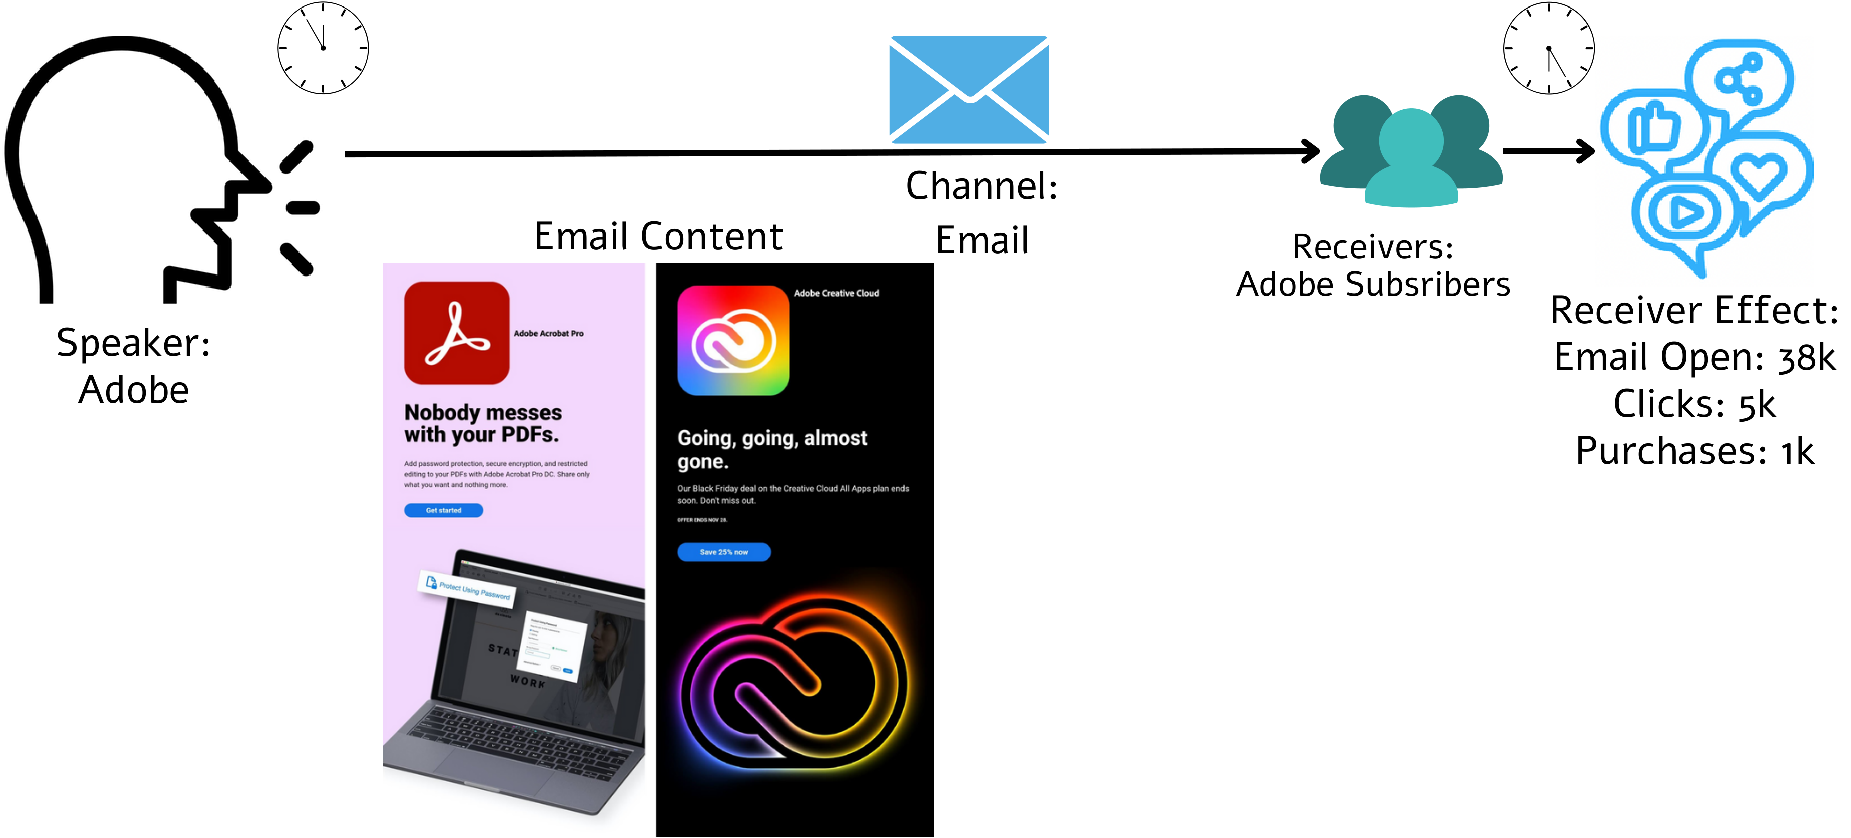
\includegraphics[width=1.0\textwidth]{images/factors of communication.pdf}
  \caption{Communication process can be defined by seven factors: Communicator, Message, Time of message, Channel, Receiver, Time of receipt, and Effect. Any message is created to serve an end goal. For marketers, the end goal is to bring in the desired receiver effect (behavior) (like clicks, purchases, likes, and customer retention). The figure presents the key elements in the communication pipeline - the marketer, message, channel, receivers, and finally, the receiver effect.   \label{fig:factors-of-communication}}
\end{figure*}


Communication includes all of the procedures by which one mind may affect another \cite{shannon-weaver-1949}. This includes all forms of expression, such as words, gestures, speech, pictures, and musical sounds.
Communication can be seen as being composed of seven parts (Fig.~\ref{fig:factors-of-communication}): (the communicator, message, time of message, channel, receiver, time of receipt, and effect). Different fields deal with different parts of communication. I will give a broad overview of these fields in the upcoming paragraphs, but two streams have emerged broadly in behavioral sciences: explanation and prediction of behavior (receiver effect) \cite{breiman2001statistical,hofman2017prediction,shmueli2010explain}. Historically, social scientists have sought explanations of human behavior that can provide interpretable causal mechanisms behind human functioning. A few prominent examples are Milgram's \cite{milgram1978obedience} and Asch's \cite{asch1948doctrine} experiments on persuasion, explaining the causal mechanism of obedience to authority. The approach of theorizing has worked in physical sciences where the data is plentiful, and theories make unambiguous predictions but has not been too successful in \textit{predicting} social outcomes in behavioral sciences \cite{open2015estimating,tetlock2017expert,forecasting2023insights}. However, causal mechanisms have their own merits; most notably, they help decision-makers (often humans) to make intuitive sense of the situation and make their next decision based on it. In parallel, due to the availability of human behavior data at scale, researchers in machine learning are showing a growing interest in traditionally social scientific topics, such as messaging strategies leading to persuasion \cite{habernal2016makes,kumar2023persuasion,luu2019measuring,bhattacharyya-etal-2023-video}, information diffusion \cite{cheng2014can,martin2016exploring}, and most importantly, prediction and predictability of human behavior \cite{choi2012predicting,song2010limits}. Machine learning approaches bring with them the culture of (training and) testing their models on large real-world datasets and pushing the state-of-the-art in terms of predictive accuracies; at the same time, often, ML approaches can only be operated as black boxes with no direct mechanism to explain predictions \cite{XXX}.



In the prediction community, different subfields have emerged dealing with the different parts of the optimization problem. For instance, advertisement personalization studies how to optimize \textit{receiver} for a given message \cite{XXX}, and recommendation systems study how to \textit{choose content} from a set of pre-decided contents for a given receiver to elicit a certain effect \cite{XXX}. A popular problem within the prediction community is the effect prediction problems, for example, clickthrough (CTR) prediction \cite{XXX}, Twitter cascade prediction \cite{cheng2014can,martin2016exploring}, sales prediction \cite{choi2012predicting,pryzant2017predicting}, content memorability prediction \cite{isola2011makes,khosla2015understanding,si2023long}, \textit{etc}. There are also works to optimize the time of the message (or receipt) to elicit certain effect \cite{XXX}. Therefore, we see that all the factors of communication are studied independently in their own light with the aim of achieving the desired effect. 


%Notably, this is the forward path of communication in which, as time progresses, a message originates, travels in a channel, is received by the subscribers, and finally generates an effect. 
Effect (or behavior) over a content can also enable us to understand about the content, the communicator, the receiver, or the time. Therefore, efforts have also been made to extract information about the content itself from the behavior it generates. For instance, using keystroke movements \cite{plank2016keystroke} and eye movements to improve natural language processing \cite{klerke2016improving,khurana-etal-2023-synthesizing}. Similarly, the fields of human alignment and reinforcement learning with human feedback (RLHF) try to use human behavioral signals of likes, upvotes, downloads, and annotations of a response's helpfulness to improve content generation - both text \cite{kreutzer2018can,stiennon2020learning,ziegler2019fine,nakano2021webgpt,si2023long} and images \cite{lee2023aligning,pressman2023simulacra,wu2023better,khurana2023behavior}.


% XXX: to be improved
In the more traditional social science and computational social science cultures, research is carried out to discover causal effects and model them. 
For instance, propaganda and mass communication studies \cite{mcquail1987mass,krippendorff2018content,lasswell1948structure,lasswell1971propaganda} try to understand the culture, time, authors, recipients in a non-invasive manner using the messages exchanged, and persuasion studies \cite{petty1981effects,chaiken1980heuristic} where the persuasion strategy present in the content is identified and correlated with (un)successful efforts of persuasion. 



A common theme that runs through both research cultures in behavioral sciences is the intent to control behavior. Explanation and prediction are intermediate steps to control and hence optimize behavior. Optimizing behavior means to fulfill the communicator's objectives by controlling the other six parts of the communication process (Fig.~\ref{fig:factors-of-communication}). Due to the problem space being large, the solution needs a general understanding of human behavior as opposed to being domain-specific. 


The characteristic that marks the digital age is the prevalence of human behavioral data in huge repositories. This data is big (allowing to model heterogeneity), always-on (allowing to look in the past as well as live measurements), observational (as opposed to reactive), but also incomplete (does not capture all that is happening everywhere everytime in a single repository) and algorithmically confounded (generated as a byproduct of an engineering process with a goal) \cite{salganik2019bit}. While the predictive culture has tried to make use of some of this data in the form of social media datasets like Twitter \cite{tumasjan2010predicting,asur2010predicting} and Instagram \cite{kim2020multimodal}, Google trends \cite{choi2012predicting,carriere2013nowcasting}, Wikipedia \cite{generous2014global,de2021general,mestyan2013early}, shopping websites \cite{krumme2013predictability,de2015unique} and other data sources \cite{brockmann2006scaling,song2010limits,miritello2013limited}, these efforts are limited, in the sense of being dependent on one or a few chosen platforms, able to answer a limited set of questions, and restricted by access to private data. We want a model that can understand (predict and explain) human behavior as opposed to modeling a particular effect (retweet prediction) on a particular platform (\textit{e.g.} Twitter) for a certain type of users.
This problem carries parallels with the problem being solved in the natural language processing (NLP) community, where supervised models in NLP are limited by the amount of supervision available and being able to answer one question (for which the supervised model was trained). The problem was solved by developing Large Language Models (LLMs), which are general purpose models capable of \textit{understanding language}, and hence can solve natural language tasks like sentiment analysis, question answering, email generation, and language translation in zero-shot (\textit{i.e.} without needing any explicit training for that task) \cite{devlin2018bert,brown2020language,radford2018improving,raffel2020exploring,radford2019language}.


Similarly, how do we develop a model capable of understanding behavior \textit{in general}? With the intent to answer this question, we take motivation from LLMs where the idea is to train a model on a data-rich task. The task chosen to train LLMs is the next-word prediction, and the dataset is the text collected from the entire internet. We leverage the human behavior repositories available on the internet for this general-purpose human behavior model. The format of this data is the general communication model shown in Fig.~\ref{fig:factors-of-communication} consisting of communicator, message, time of message, channel, receiver, time of receipt, and effect. Due to the incomplete nature of behavioral repositories, all the factors are usually not always available. However, a subset is always available, and we show that the data scale helps make a general behavior understanding model \cite{khandelwal2023large}. We show that the model is capable of predicting behavior, explaining it, and also generating message to bring about certain behavior \cite{khurana2023behavior,si2023long,khandelwal2023large}.



Following the two traditions of social sciences, in this work, in Chapter-\ref{chatper:Explaining Behavior: Persuasion Strategies}, I start with a more traditional approach to behavior explanation, where I cover the first works on extracting persuasion strategies in advertisements (both images and videos) \cite{kumar2023persuasion,bhattacharyya-etal-2023-video}. The contributions of these works include constructing the largest set of generic persuasion strategies based on theoretical and empirical studies in marketing, social psychology, and machine learning literature and releasing the first datasets to enable the study and model development for the same. These works have been deployed to understand the correlation between the kinds of marketing campaigns and customer behavior measured by clicks, views, and other marketing key performance indicators (KPIs). 

Following this, in Chapter-\ref{chatper:Content and Behavior Models}, I delve into the more modern approach of behavior prediction and leveraging the huge repositories of behavior data available. First, we propose models to integrate behavior with relatively smaller language models like BERT \cite{devlin2018bert}, and show that the resultant models can understand content better than the base models \cite{khurana-etal-2023-synthesizing}. Then, we propose an approach to integrate behavior and content together as part of a single model. We call these models Large Content and Behavior Models (LCBM) \cite{khandelwal2023large}. We show that these models can predict and explain behavior. Next, in Chapter-\ref{chatper:Generating Content Leading to Optimal Behavior}, we show that using these models we can generate messages to elicit certain behavior resulting in behavior optimization. We show this both for the domain of text, by taking the illustrative case of memorability and generating content that is more memorable in long-term \cite{si2023long}, and images, by generating images that are more performant, \textit{i.e.}, can result in more likes and downloads \cite{khurana2023behavior}.



\begin{comment}
    They mentioned that the broad problem of communication can be studied at three levels: technical, semantic, and effectiveness. 
    \textbf{Level A: Technical.} How accurately can the symbols of communication be transmitted?
    
    \textbf{Level B: Semantic.} How precisely do the transmitted symbols convey the desired meaning?
    
    \textbf{Level C: Effectiveness.} How well does the received meaning induce the desired conduct in the receiver?
    
    These three levels build on top of each other. Thus, solving the problem at Level C necessarily requires solving the corresponding problems at Levels A and B.
    
    Since the publication of this seminal paper, the tremendous growth in the field of telecommunications, particularly the advent of the Internet and mobile devices, has led to affordable, wide-scale solutions for Level A.
    With the recent advances in large language models (LLMs) such as BERT \citep{devlin2018bert}, GPT-3 and 4 \citep{brown2020language,openai2023gpt4}, T5 \citep{raffel2020exploring}, and many more, we have witnessed a significant improvement in the performance of various Natural Language Processing (NLP) tasks. LLMs in zero- or few-shot settings can easily handle tasks such as question answering, summarization, translation, and many more. This has helped us progress towards solving Level B to a large extent. However, there has been limited progress in Level C, the effectiveness problem. 
    
    
    
    Effectiveness refers to communicating to fulfill the communicator's objectives.
\end{comment}


%%%%%%%%%%%%%%%%%%%%%%%%%%%%%%%%%%%%%%%%
%%%%%%%%%%%%%%%%%%%%%%%%%%%%%%%%%%%%%%%%
%%%%%%%%%%%%%%%%%%%%%%%%%%%%%%%%%%%%%%%%
%%%%%%%%%%%%%%%%%%%%%%%%%%%%%%%%%%%%%%%%

\chapter{Explaining Behavior: Persuasion Strategies}
\label{chatper:Explaining Behavior: Persuasion Strategies}


\begin{figure}[t]
    % \vspace{-38mm}
    \centering
    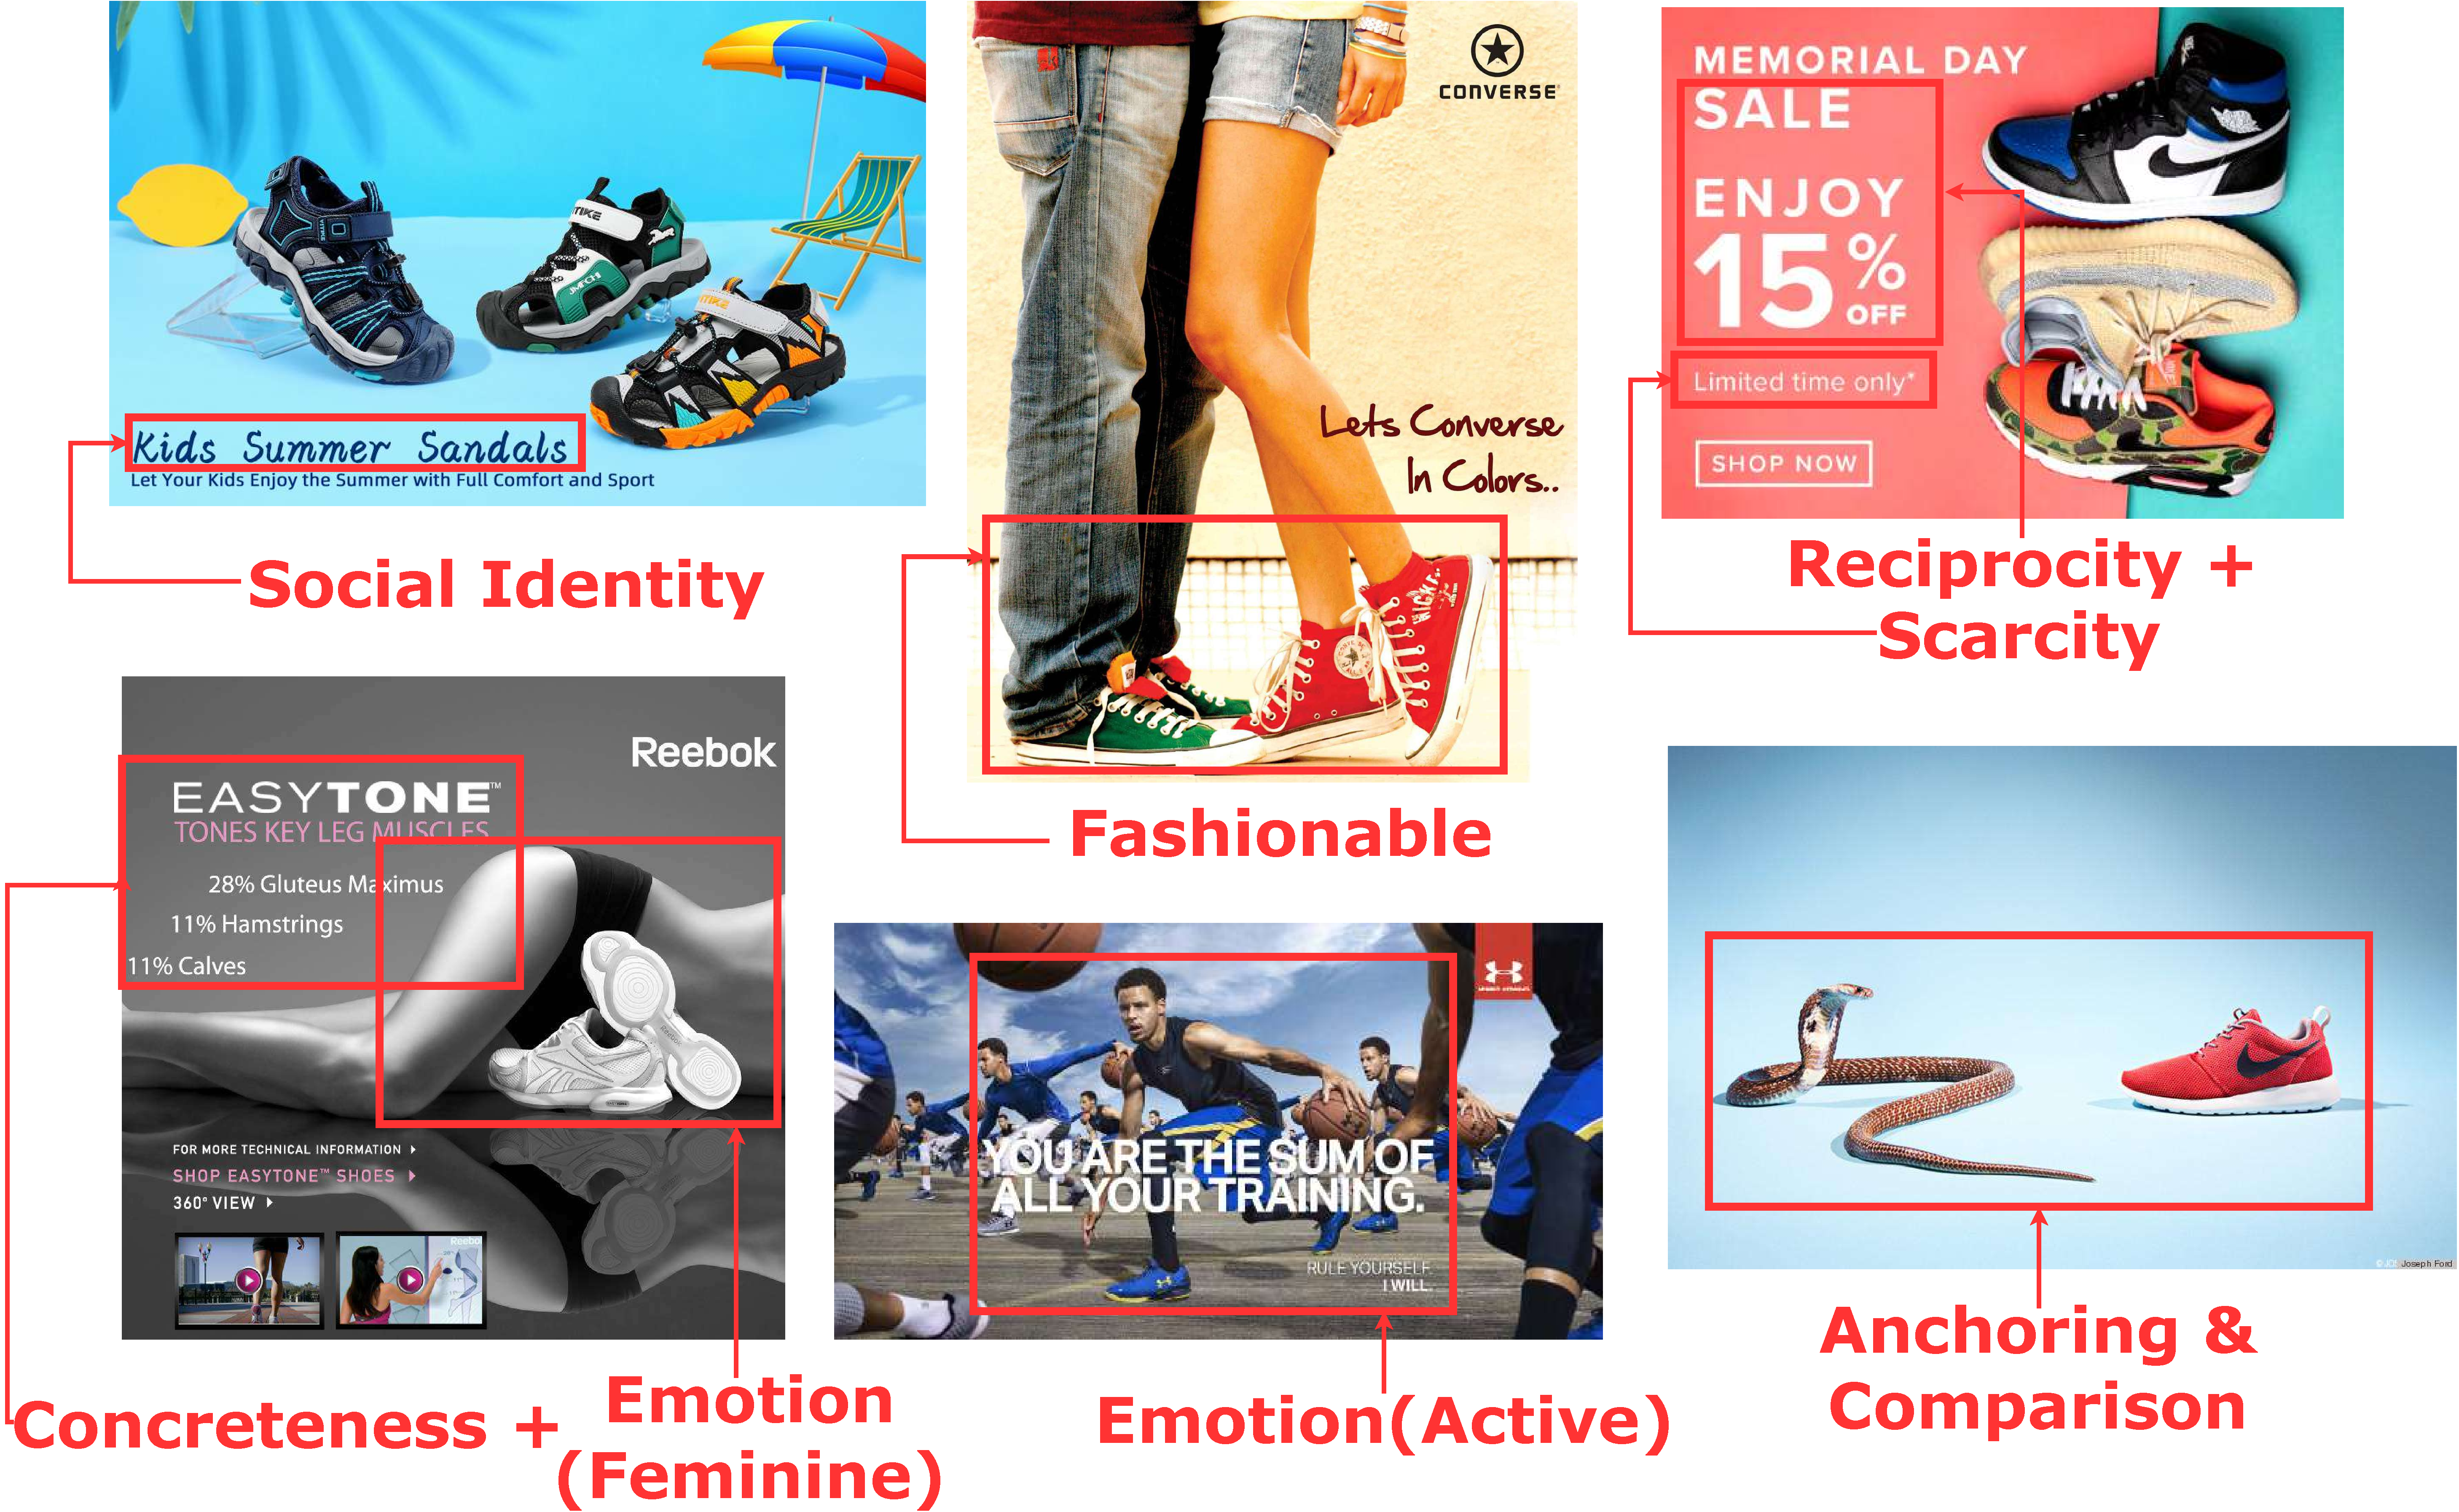
\includegraphics[scale=0.08]{images/footwear-strategies.pdf}
    \caption{Different persuasion strategies are used for marketing the same product (footwear in this example). The strategies are in red words and to be defined by us in the paper.}
    \label{fig:footwear-strategies}
    % \vspace*{-4mm}
\end{figure}


\begin{figure*}[!ht]
    \centering
    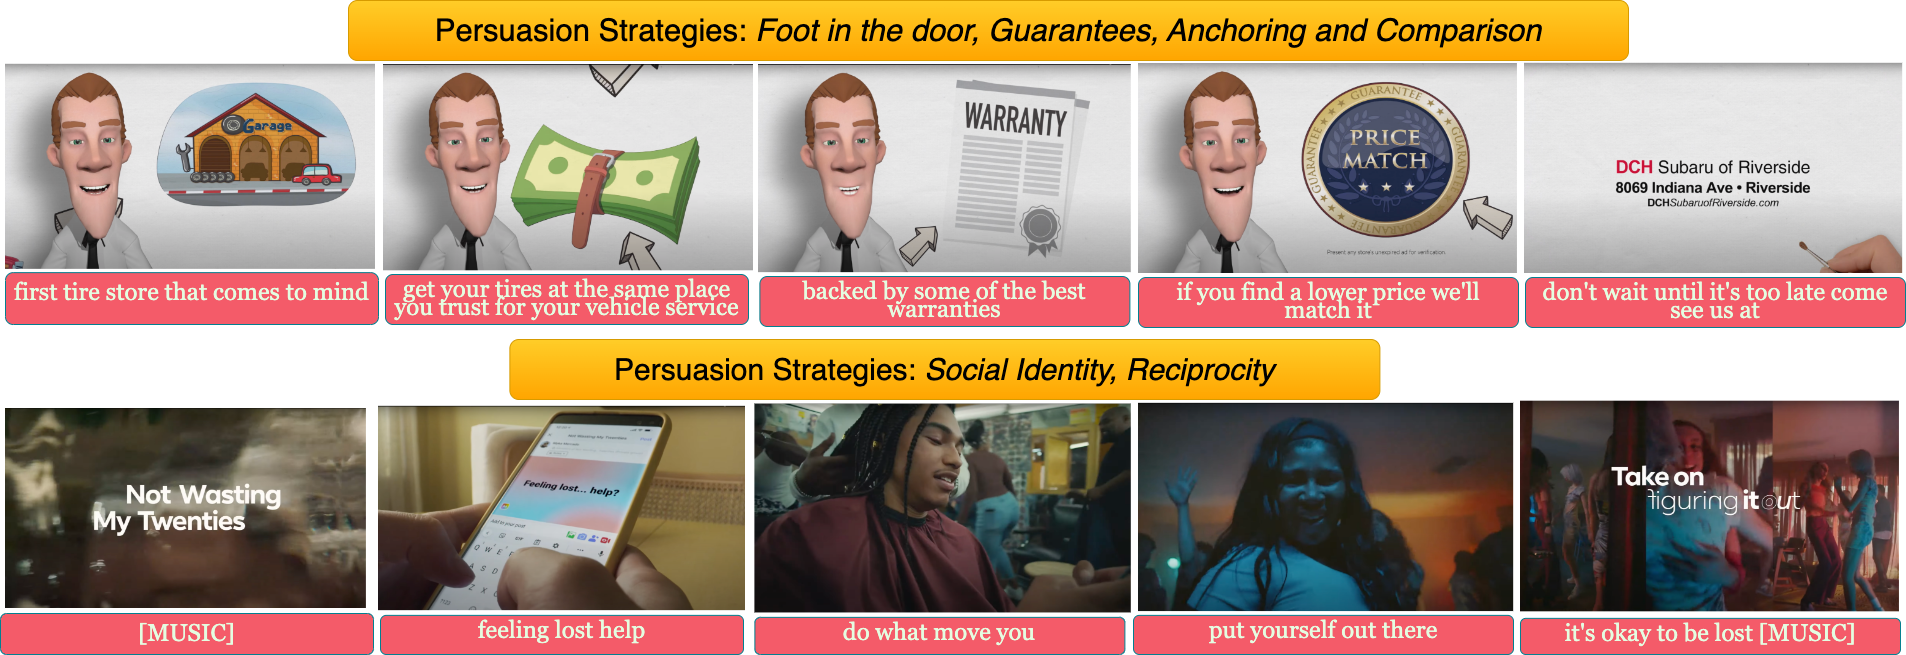
\includegraphics[width=\textwidth]{images/persuasion-strategies-videos.png}
    \caption{Examples of videos with their annotated persuasion strategies. Relevant keyframes and ASR captions are shown in the figure, along with the annotated strategies. These two videos can be watched at 
    \url{https://bit.ly/3Ie3JG0}, \url{https://bit.ly/3OgtLwj}
    .}
    \label{fig:persuasion-strategy-dataset-examples}
\end{figure*}



 Modeling what makes an advertisement persuasive, \textit{i.e.}, eliciting the desired response from consumer, is critical to the study of propaganda, social psychology, and marketing. Despite its importance, computational modeling of persuasion in computer vision is still in its infancy, primarily due to the lack of benchmark datasets that can provide persuasion-strategy labels associated with ads. Motivated by persuasion literature in social psychology and marketing, we introduce an extensive vocabulary of persuasion strategies and build the first ad corpus (both image and video) annotated with persuasion strategies. We then formulate the task of persuasion strategy prediction with multi-modal learning. The image dataset also provides image segmentation masks, which labels persuasion strategies in the corresponding ad images on the test split. We publicly release our code and dataset at \url{https://midas-research.github.io/persuasion-advertisements/}. This chapter is based on two papers I published along with collaborators \cite{kumar2023persuasion,bhattacharyya-etal-2023-video}.




Marketing communications is the mode by which companies and governments inform, remind, and persuade their consumers about the products they sell. They are the primary means of connecting brands with consumers through which the consumer can know what the product is about, what it stands for, who makes it, and can be motivated to try it out. To introduce meaning into their communication, marketers use various rhetorical devices in the form of persuasion strategies such as \textbf{emotions} ({\it e.g.}, Oreo's ``Celebrate the Kid Inside'', humor by showing Ronald McDonald sneaking into the competitor Burger King's store to buy a burger), \textbf{reasoning} ({\it e.g.}, ``One glass of Florida orange juice contains 75\% of your daily vitamin C needs''), \textbf{social identity} ({\it e.g.}, Old Spice's ``Smell like a Man''), and \textbf{impact} ({\it e.g.}, Airbnb showing a mother with her child with the headline ``My home is funding her future'') (Refer to Fig.~\ref{fig:rhetoric-strategies-ads} to see these ads). Similarly, even for marketing the same product, marketers use different persuasion strategies to target different demographies (see Fig.~\ref{fig:footwear-strategies}). Therefore, recognizing and understanding persuasion strategies in ad campaigns is vitally important to decipher viral marketing campaigns, propaganda, and enable ad-recommendation. 




\begin{figure*}
    \centering
    \begin{subfigure}[b]{0.22\textwidth}
         \centering
         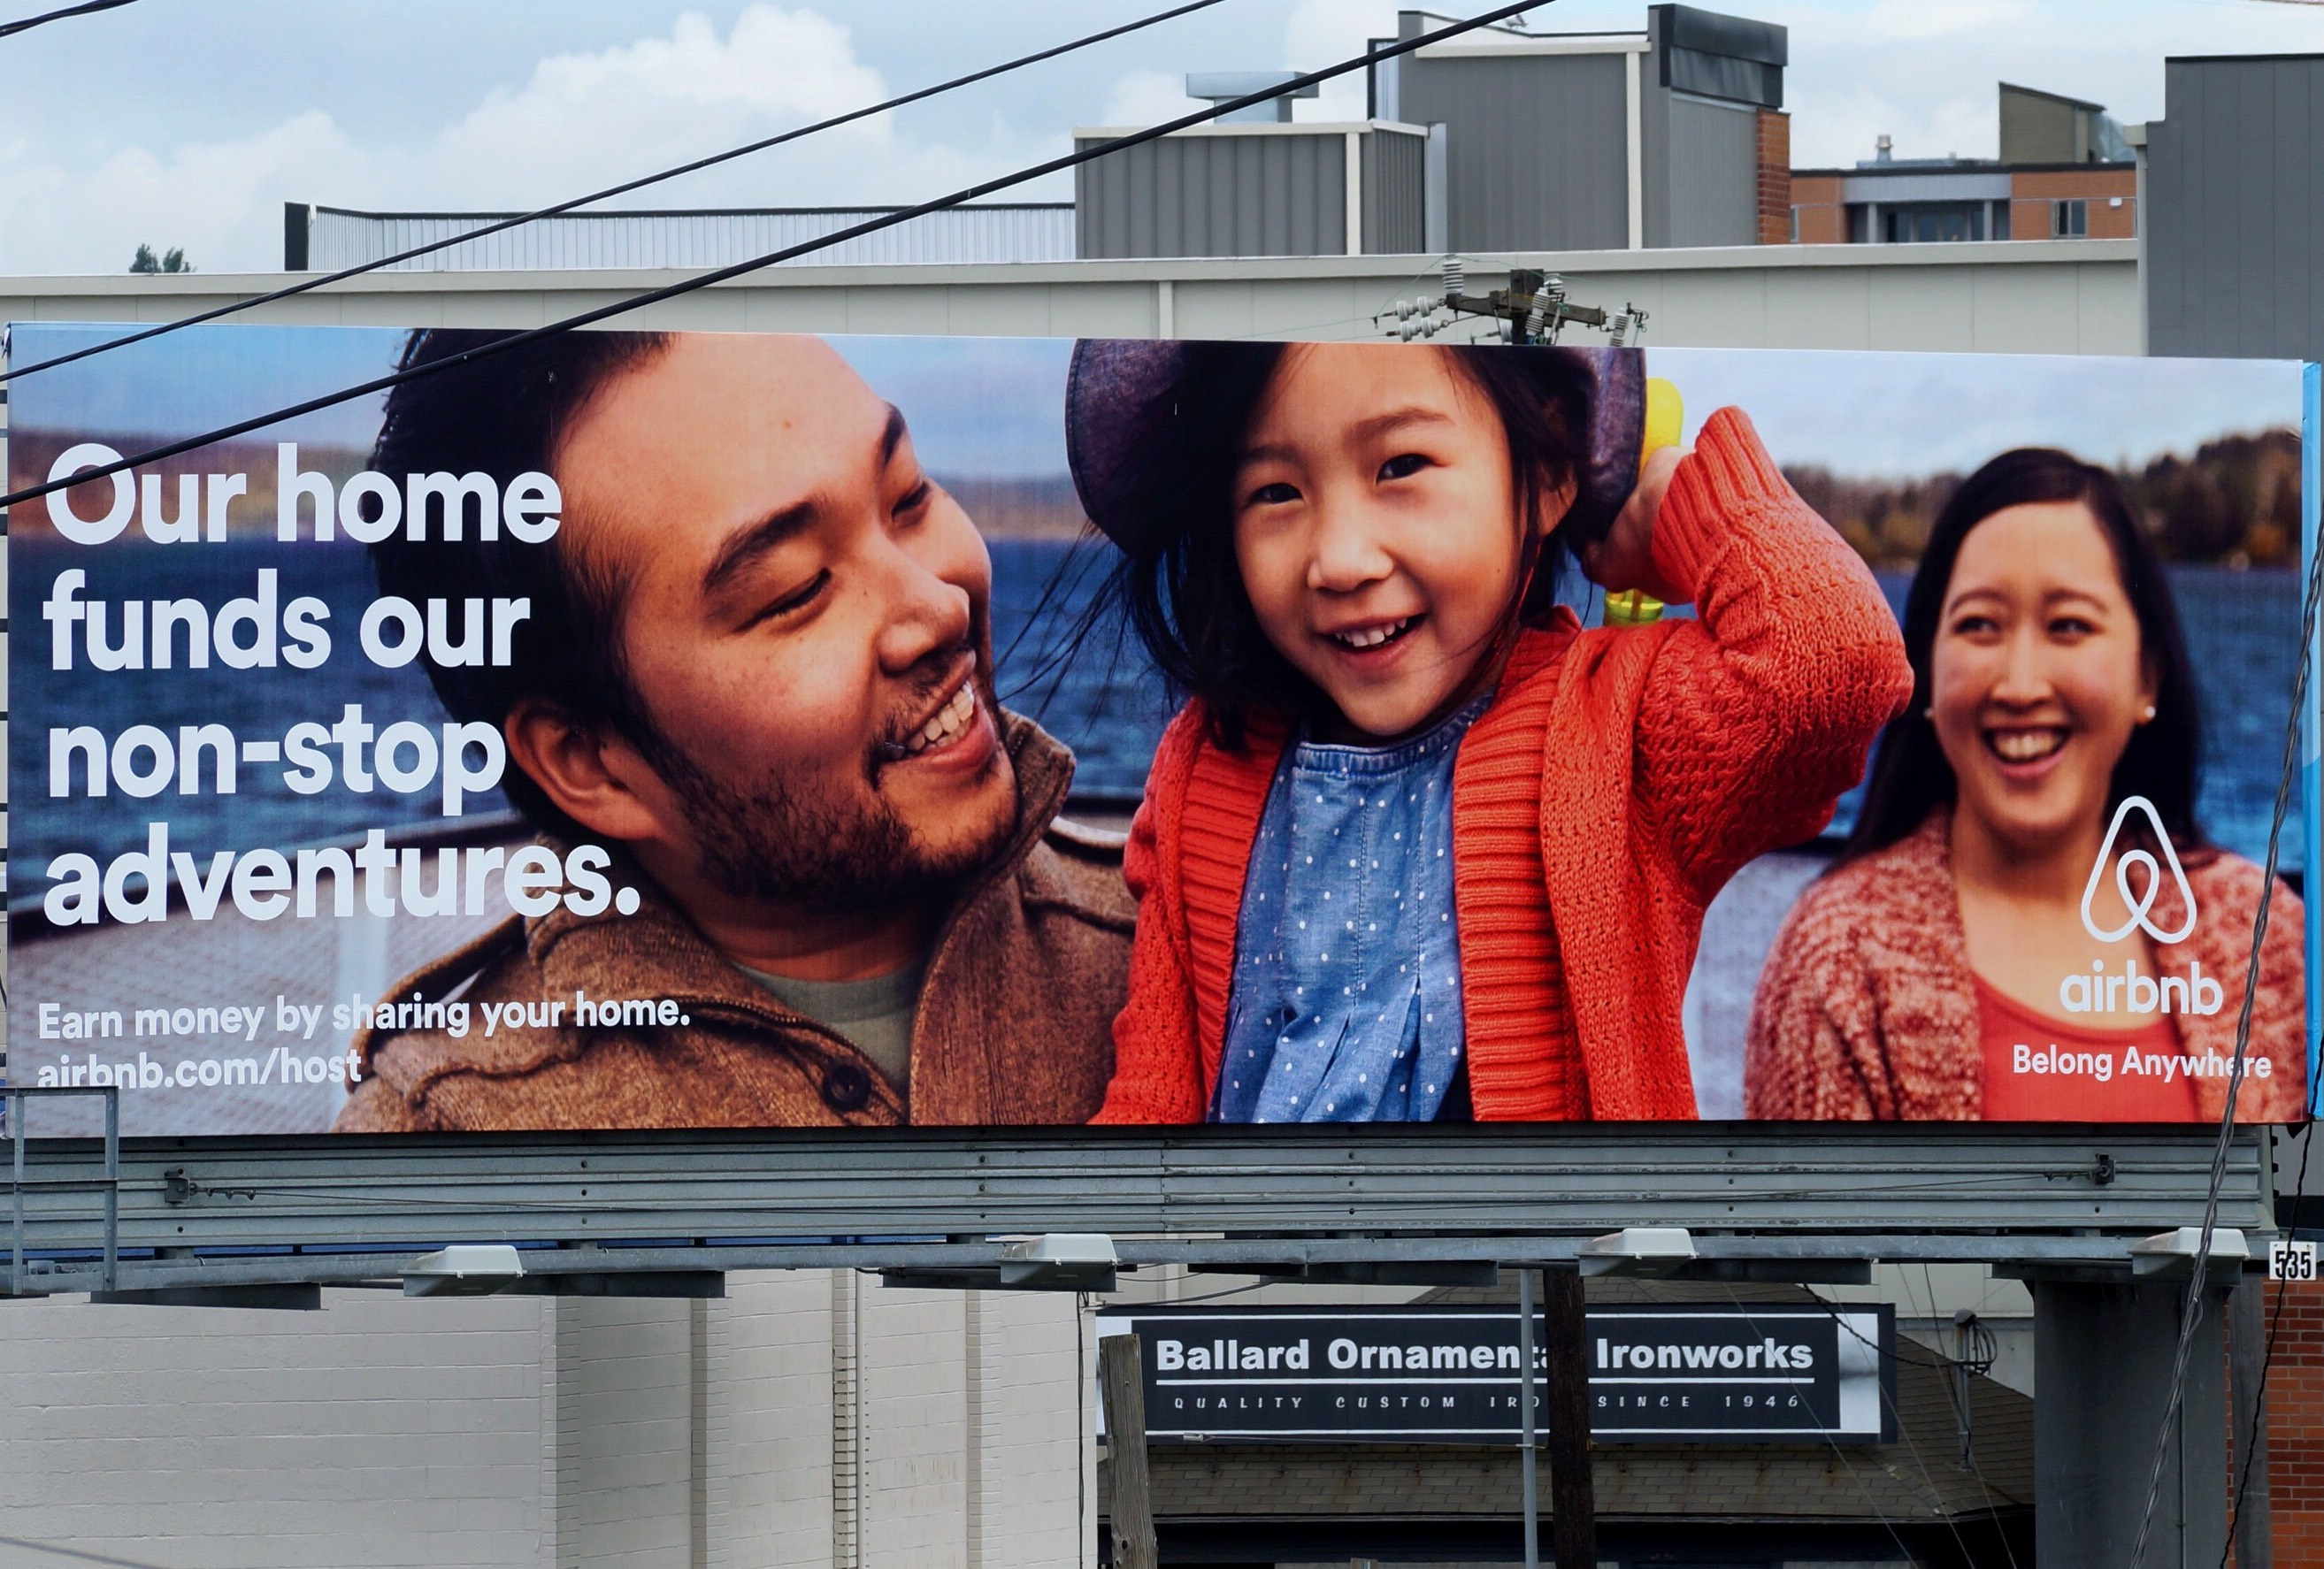
\includegraphics[width=\textwidth,scale=0.6]{images/airbnb.jpeg}
         \caption{}
         \label{fig:Airbib}
     \end{subfigure}
     \begin{subfigure}[b]{0.2\textwidth}
         \centering
         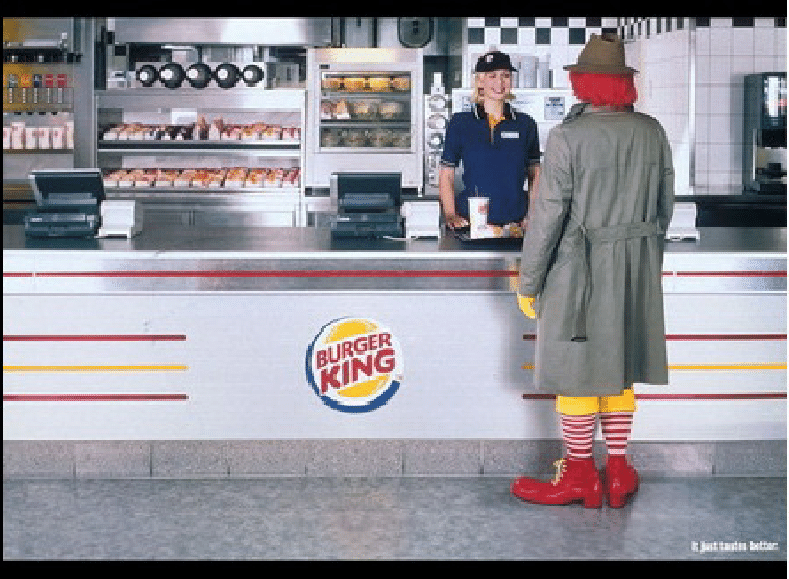
\includegraphics[width=\textwidth,scale=0.5]{images/Burger-King-vs-McDonalds-comparative-ad.png}
         \caption{}
         \label{fig:mcdonald}
     \end{subfigure}
     \begin{subfigure}[b]{0.27\textwidth}
         \centering
         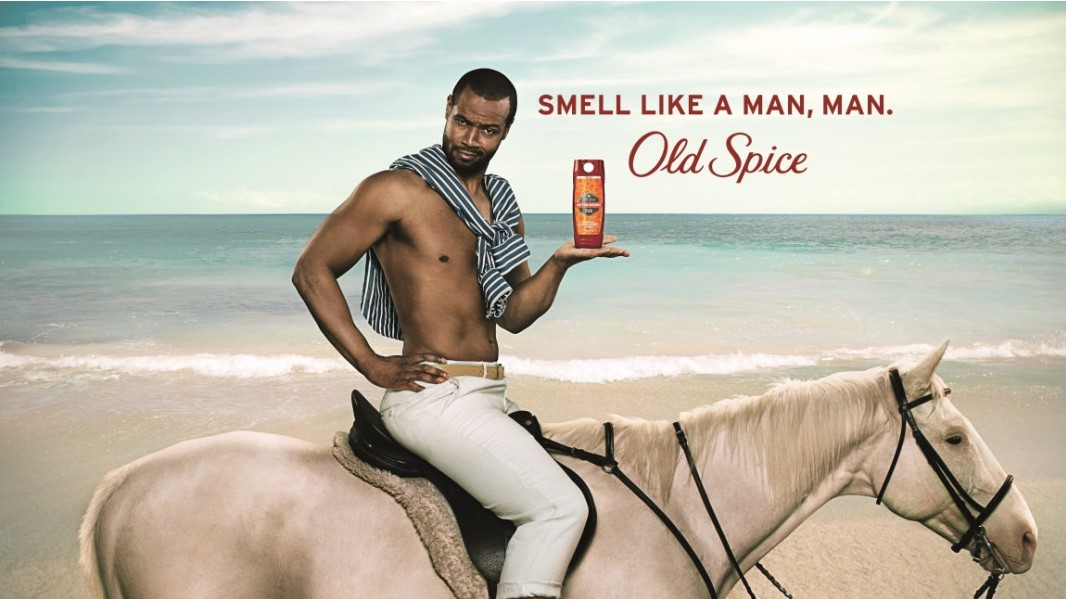
\includegraphics[width=\textwidth,scale=1.0]{images/old-spice.jpeg}
         \caption{}
         \label{fig:old-spice}
     \end{subfigure}
     \begin{subfigure}[b]{0.12\textwidth}
         \centering
         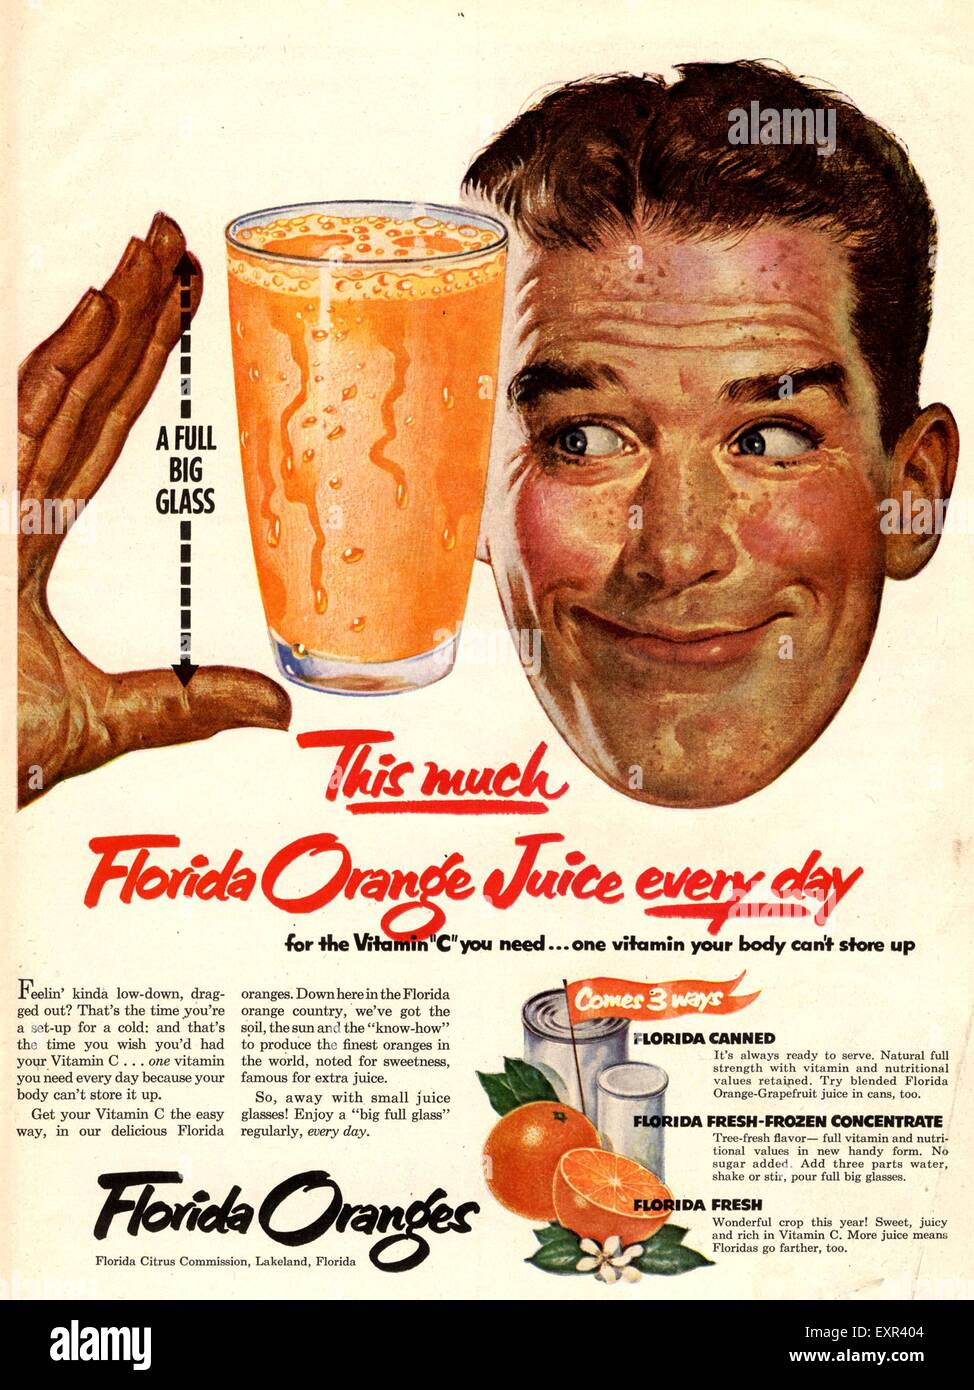
\includegraphics[width=\textwidth,scale=0.68]{images/1950s-usa-florida-orange-juice-magazine-advert-EXR404.jpeg}
         \caption{}
         \label{fig:florida-juice}
     \end{subfigure}
     \begin{subfigure}[b]{0.12\textwidth}
         \centering
         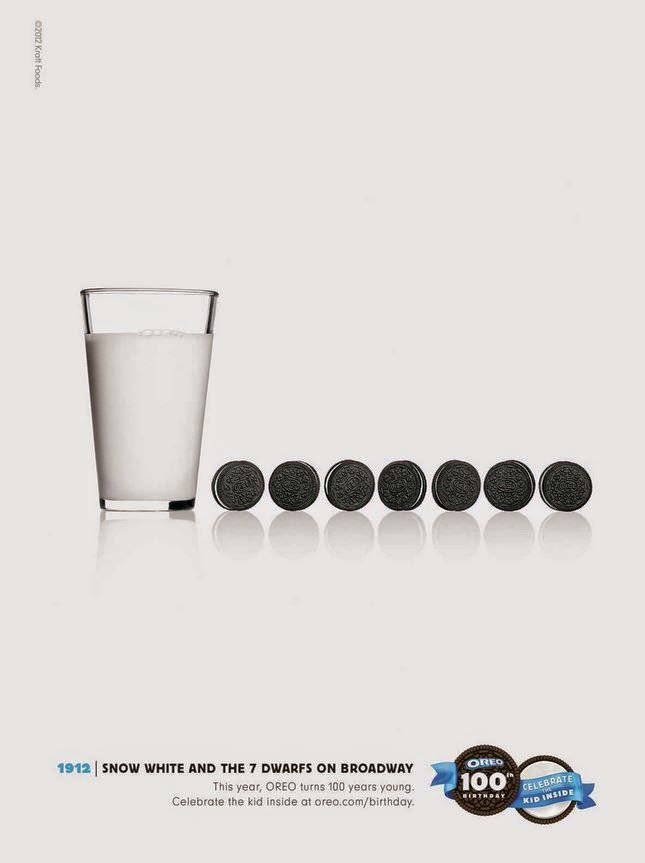
\includegraphics[width=\textwidth,scale=0.68]{images/Oreo_SnowWhite.jpeg}
         \caption{}
         \label{fig:oreo}
     \end{subfigure}
     
     
    \caption{Various rhetoric strategies used in advertisements}
    \label{fig:rhetoric-strategies-ads}
\end{figure*}




Studying rhetorics of this form of communication is an essential part of understanding visual communication in marketing. Aristotle, in his seminal work on rhetoric, underlining the importance of persuasion, equated studying rhetorics with the study of persuasion\footnote{``Rhetoric may be defined as the faculty of discovering in any particular case all of the available means of \textit{persuasion}'' \cite{rapp2002aristotle}} \cite{rapp2002aristotle}. While persuasion is studied extensively in social science fields, including marketing \cite{meyers1999consumers,keller2003affect} and psychology \cite{hovland1953communication,petty1986elaboration}, computational modeling of persuasion in computer vision is still in its infancy, primarily due to the lack of benchmark datasets that can provide representative corpus to facilitate this line of research. In the limited work that has happened on persuasion in computer vision, researchers have tried to address the question of which image is more persuasive \cite{bai2021m2p2} or extracted low-level features (such as emotion, gestures, and facial displays), which indirectly help in identifying persuasion strategies without explicitly extracting the strategies themselves \cite{joo2014visual}. On the other hand, decoding persuasion in textual content has been extensively studied in natural language processing from both extractive, and generative contexts \cite{habernal2016makes,ChenYang2021,luu2019measuring}. This forms the motivation of our work, where we aim to identify the persuasion strategies used in visual content such as advertisements.




%In the limited work which has happened in computer vision domain for studying advertisements, researchers have investigated topics, sentiments, action-reason (containing \textit{what} the viewer should do and \textit{why} they should do it, according to the ad) statements \cite{hussain2017automatic,ye2018advise,ye2019interpreting}, or other features such as emotion, gestures, and facial display types in ads \cite{huang2016inferring,joo2014visual,DBLPconfbmvc0004K18}. While the prior computer vision work was important for finding the lower-level content properties of advertisements, studying advertisement rhetoric involves integrating the above lower-level elements to form \textit{persuasive message appeals}. %atkinson2019gets,carlile2018give,stab2014annotating,althoff2014ask,iyer2019unsupervised,rosenthal2017detecting,yang2019let,stab2017parsing,tan2016winning,wang-etal-2019-persuasion,zhang2016inferring,duerr2021persuasive,anand2011believe,chen2021weakly,hidey2017analyzing,he2018decoupling,durmus-cardie-2018-exploring,wachsmuth2017computational,longpre2019persuasion,shaikh-etal-2020-examining} use cases, and in  %




The systematic study of persuasion began in the 1920s with the media-effects research by Lasswell \cite{lasswell1971propaganda}, which was used as the basis for developing popular models of persuasion, like the Elaboration Likelihood Model (ELM) \cite{petty1986elaboration}, Heuristic Systematic Model (HSM) \cite{chaiken1980heuristic}, and Hovland's attitude change approach \cite{hovland1953communication}. %Amongst these, the most widely accepted model of persuasion theory is the Elaboration Likelihood Model (ELM). 
Laswell in this research broke down communication into five factors by defining communication as an act of \textit{who} said it, \textit{what} was said, in \textit{what} channel it was said, to \textit{whom} it was said, and with what \textit{effect} it was said. Later, this model was used as the basis for developing popular models of persuasion, like Elaboration Likelihood Model \cite{petty1986elaboration}, Heuristic Systematic Model \cite{chaiken1980heuristic}, and Hovland's attitude change approach \cite{hovland1953communication}. Amongst these, the most widely accepted model of persuasion theory is the Elaboration Likelihood Model (ELM). 

These models of persuasion posit a dual process theory that explains attitude and behavior change (persuasion) in terms of the following major factors: stimuli (messages), personal motivation (the desire to process the message), capability of critical evaluation, and cognitive busyness. These factors could be divided into cognitive, behavioral, and affective processes of attitude change. 
Thus, a person may begin liking a new political candidate because she just donated \$100 to the campaign (behavior-initiated change), because the theme music in a recently heard commercial induced a general pleasantness (affect-initiated change), or because the person was impressed with the candidate’s issue positions (cognitive initiated change). Similarly, if a person already likes a political candidate he may agree to donate money to the campaign (behavioral influence), may feel happiness upon meeting the candidate (affective influence), and may selectively encode the candidate’s issue positions (cognitive influence) \cite{petty1986elaboration}.

ELM posits that when facing a message from a persuader, the persuadee reacts by using the two information processing channels: central processing or peripheral processing. When the persuadee processes information centrally, the cognitive responses, or elaborations, will be much more relevant to the information, whereas when processing peripherally, the individual may rely on heuristics and other rules of thumb when elaborating on a message. The factors which influence how and how much one will elaborate the persuasive message is given by the message type, personal motivation, and other factors presented in the ELM. Being at the high end of the elaboration continuum, people assess object-relevant information in relation to schemas that they already possess, and arrive at a reasoned attitude that is supported by information \cite{van2011handbook}. 

In this chapter, we build on these psychological insights from persuasion models in sociology and marketing and study the message strategies that lead to persuasion. We codify, extend, and unify persuasion strategies studied in the psychology and marketing literature into a set of 20 strategies divided into 9 groups (see Fig.~\ref{fig:persuasion-strategies-headline-image}, Table~\ref{tab:persuasive-strategies-list}): \textit{Authority and Credibility}, \textit{Social Identity and Proof}, where cognitive indirection in the form of group decisioning and expert authority is used for decisions, \textit{Value and Impact Formulation} where logic is used to explain details and comparisons are made, \textit{Reciprocity}, \textit{Foot in the door}, \textit{Overcoming Resistance} where social and cognitive consistency norms are harnessed to aid decision-making, \textit{Scarcity}, \textit{Anthropomorphism} and \textit{Emotion} where information is evaluated from the lenses of feelings and emotions. In addition to introducing the most extensive vocabulary for persuasion strategies, we make a superset of persuasion strategies presented in the prior NLP works, which introduced text and domain-specific
persuasion tactics, thus making large-scale understanding of persuasion across multiple contexts comparable and replicable.


Constructing a large-scale dataset containing persuasion strategies labels is time-consuming and expensive. We leverage active learning to mitigate the cost of labeling fine-grained persuasion strategies in advertisements. We first introduce an attention-fusion model trained in a multi-task fashion over modalities such as text, image, and symbolism. We use the action-reason task from the Pitts Ads dataset \cite{hussain2017automatic} to train the model and then annotate the raw ad images from the same dataset for persuasion strategies based on an entropy based active learning technique.


%As an interesting use case, we extract 1600 raw ad images of Fortune-500 companies using the Facebook Ads API\footnote{\url{https://www.facebook.com/ads/library/api/}}. Then, using the model trained for persuasion strategies, we labelled and analyzed the advertisement campaigns on different companies and industry segments. We find that (\S\ref{sec:Case Study}).


To sum up, our contributions include:\\
1. We construct the largest set of generic persuasion strategies based on theoretical and empirical studies in marketing, social psychology, and machine learning literature. \\
2. We introduce the first dataset for studying persuasion strategies in advertisements. This enables initial progress on the challenging task of automatically understanding the messaging strategies conveyed through visual advertisements. We also construct a prototypical dataset containing image segmentation masks annotating persuasion strategies in different segments of an image.\\
3. We formulate the task of predicting persuasion strategies with a multi-task attention fusion model.\\
4. We conduct extensive experiments on the released corpus,
showing the effect of different modalities on identifying persuasion
strategies, correlation between strategies and topics
and objects with different strategies.\\

\begin{figure*}[t]
% \vspace*{-12mm}
        \centering
        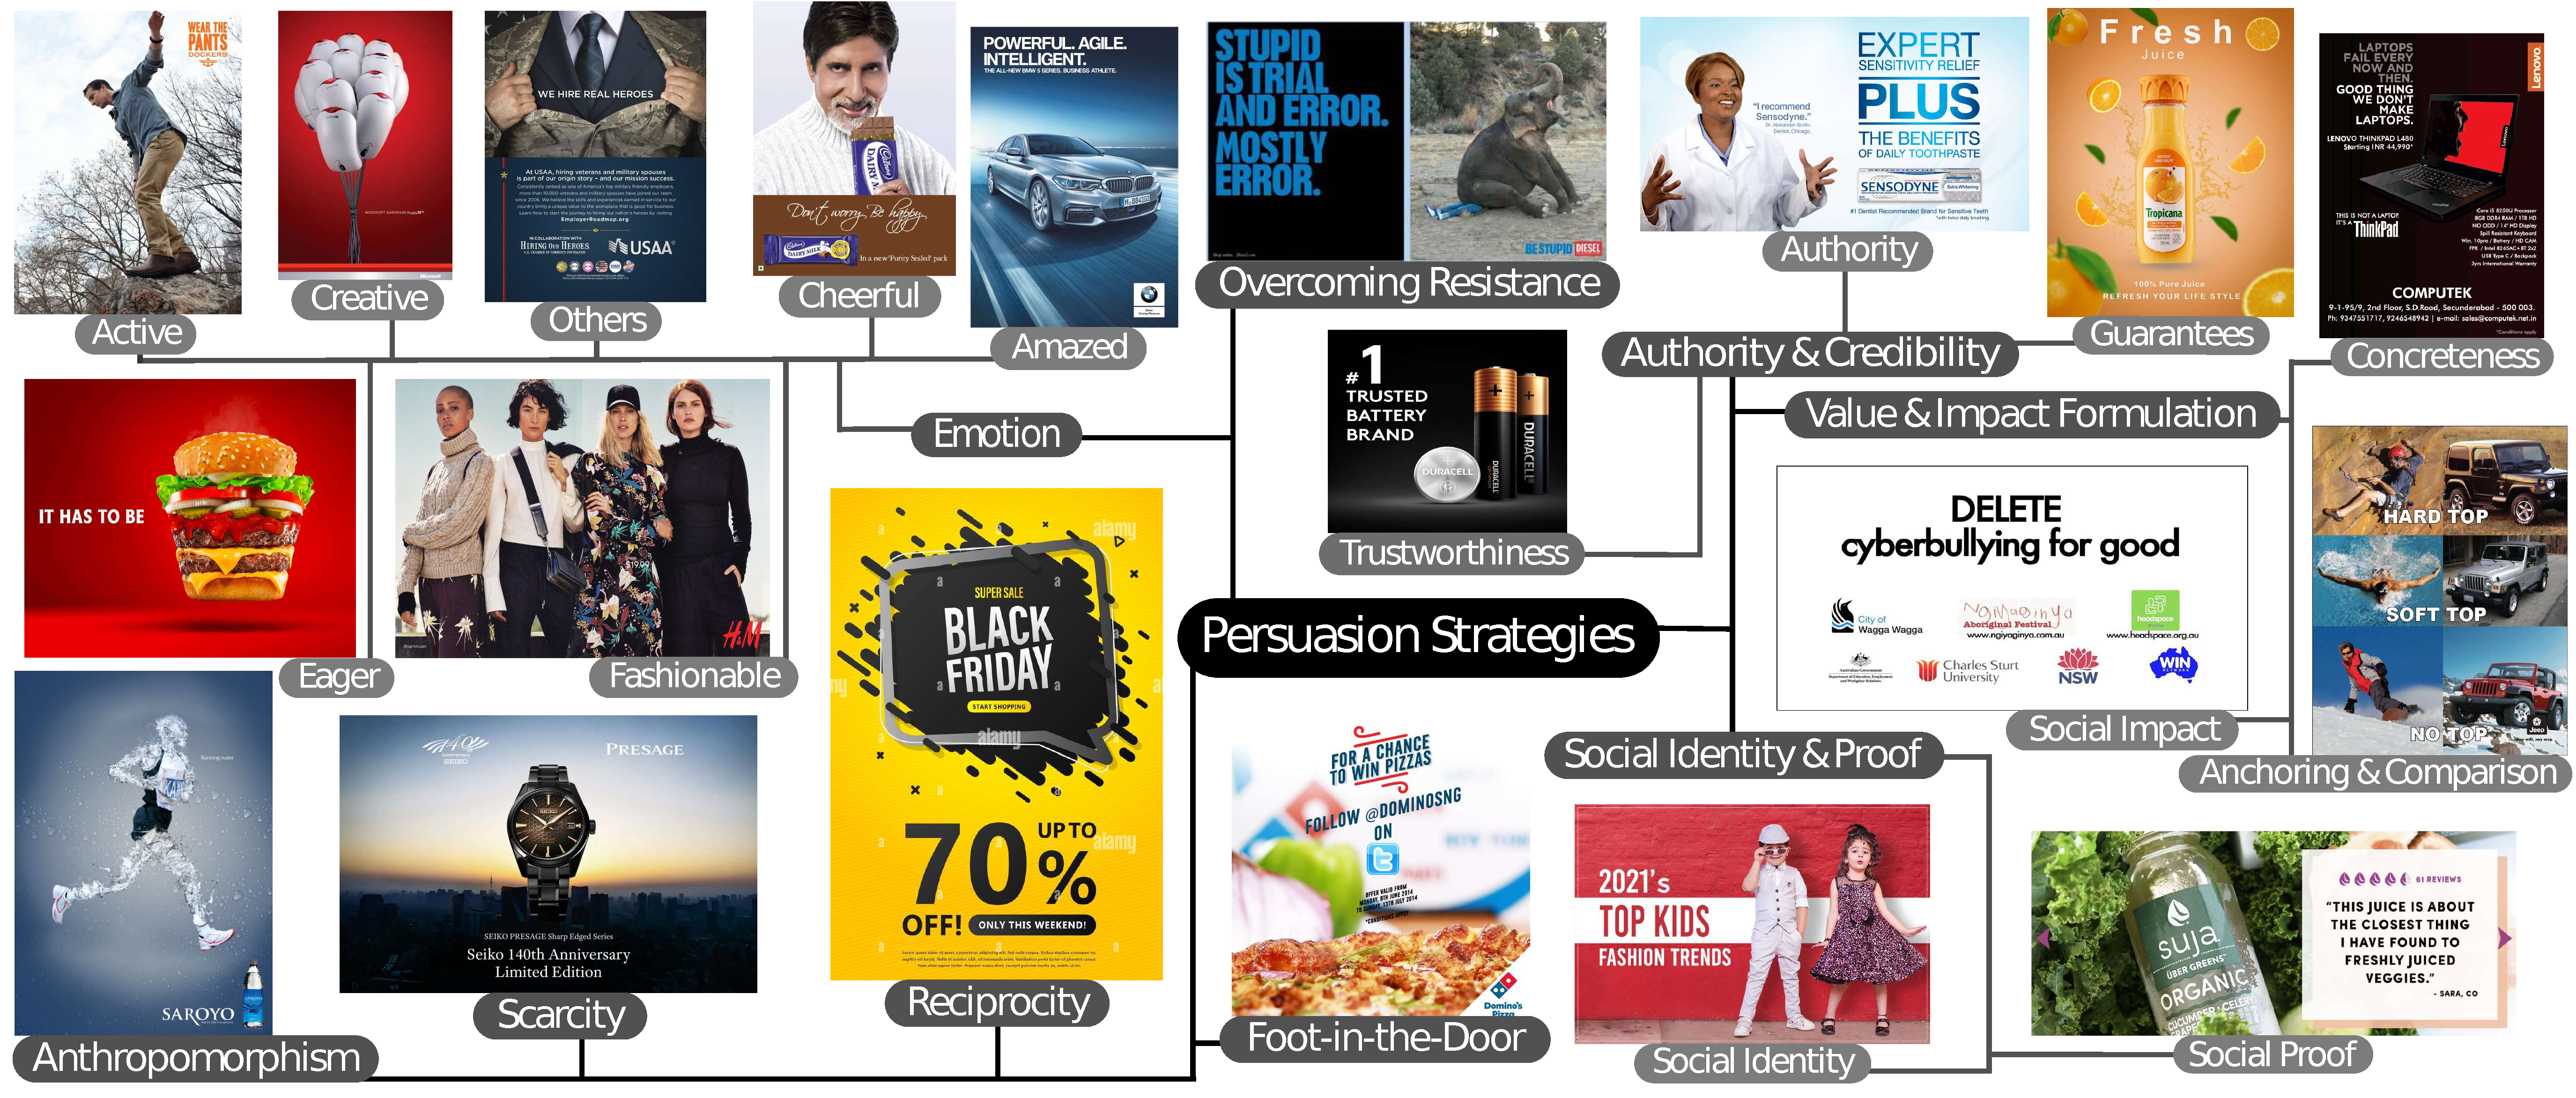
\includegraphics[width=\textwidth]{images/flowchart.pdf}
        \caption{\small \looseness=-1 Persuasion strategies in advertisements. Marketers use both text and vision modalities to create ads containing different messaging strategies. Different persuasion strategies are constituted by using various rhetorical devices such as slogans, symbolism, colors, emotions, allusion.}
        \label{fig:persuasion-strategies-headline-image}
% \vspace*{-4mm}
\end{figure*}

\section{Related Work}
\label{sec:related work}


\textit{How do messages change people's beliefs and actions?} The systematic study of persuasion has captured researchers’ interest since the advent of mass influence mechanisms such as radio, television, and advertising. Work in persuasion spans across multiple fields, including psychology, marketing, and machine learning. 


\textbf{Persuasion in Marketing and Social Psychology:} Sociology and communication science has studied persuasion for centuries now starting from the seminal work of Aristotle on rhetoric. Researchers have tried to construct and validate models of persuasion. Due to space constraints, while we cannot cover a complete list of literature, in Section~\ref{tab:persuasive-strategies-list}, we list the primary studies which originally identified the presence and effect of various persuasion tactics on persuadees. We build on almost a century of this research and crystallize them into the persuasion strategies we use for annotation and modeling. %Using both expenditure and income calculations, \citet{mccloskey1995one} calculate that roughly one quarter of the US GDP in 1994 was due to persuasion. 
Any instance of (successful) persuasion is composed of two events: (a) an attempt by the persuader, which we term as the persuasion strategies, and (b) subsequent uptake and response by the persuadee \cite{anand2011believe,vakratsas1999advertising}. In this work, we study (a) only while leaving (b) for future work. Throughout the rest of the paper, when we say persuasion strategy, we mean the former without considering whether the persuasion was successful or not. 



\textbf{Persuasion in Machine Learning:} Despite extensive work in social psychology and marketing on persuasion, most of the work is qualitative, where researchers have looked at a small set of messages with various persuasion strategies to determine their effect on participants. Computational modeling of persuasion is still largely lacking. In the limited work in computational modeling of persuasion, almost all of it is concentrated in the NLP literature, with only very few works in computer vision.
Research on persuasion in NLP under the umbrella of argumentation mining is broadly carried out from three perspectives: extracting persuasion tactics, studying the effect of constituent factors on persuasion, and measurement of persuasiveness nature of content. A few examples of research studies that annotate persuasive strategies in various forms of persuader-persuadee interactions like discussion forums, social media, blogs, academic essays, and debates are \cite{anand2011believe,tan2016winning,chen2021weakly}. We use these and other studies listed in Section~\ref{tab:persuasive-strategies-list} to construct our vocabulary of persuasion strategies in advertisements. 

Other studies focus on factors such as argument ordering \cite{shaikh-etal-2020-examining,li-etal-2020-exploring-role}, target audience \cite{lukin-etal-2017-argument}, and prior beliefs \cite{el-baff-etal-2020-analyzing} for their effect in bringing about persuasion. Studies such as \cite{althoff2014ask,wei2016post} also try to measure persuasiveness and generate persuasive content. The generation of persuasive (textual) messages has been studied \cite{donadello2020explaining} and, in particular, a novel ML method for learning user model tailored persuasion strategy has also been proposed \cite{hadoux2021strategic, donadello2022machine}.



As one of the first works in the limited work in the computer vision domain, Joo \textit{et al.} \cite{joo2014visual} introduced syntactical and intent features such as facial displays, gestures, emotion, and personality, which result in persuasive images. Their analysis was done on human images, particularly politicians, during their campaigns. %\citet{huang2016inferring} built on top of their dataset to improve their results by using finetuned CNNs. 
Their work on political campaigners is more restrictive than general product and public-service advertisements. Moreover, they deal with low-level features such as gestures and personality traits depicted through the face, which are important for detecting persuasion strategies but are not persuasion strategies themselves. Recently, Bai \textit{et al.} \cite{bai2021m2p2} studied persuasion in debate videos where they proposed two tasks: debate outcome prediction and intensity of persuasion prediction. Through these tasks, they predict the persuasiveness of a debate speech, which is orthogonal to the task of predicting the strategy used by the debater. Other similar works which discuss persuasiveness of images and videos are \cite{joo2015automated,siddiquie2015exploiting}.


%\noindent \textbf{Active Learning} tackles the problem of selecting samples from unlabeled sets to be annotated by an oracle. In the last decade, several active learning strategies have been proposed and applied to several research fields, including speech recognition \cite{hakkani2002active}, natural language processing \cite{thompson1999active}, chemistry \cite{duros2017human}. We refer the reader to the survey of \citet{settles2009active} for an extensive review of active learning methods. Many studies including \citet{collins2008towards,miller_linder_mebane_2020,mullapudi2021learning} have practically applied active learning to annotate datasets and shown substantial improvement in labelling budget and time. 




\section{Generic Taxonomy of Persuasion Strategies}
\label{tab:persuasive-strategies-list}
This section introduces the generic taxonomy of persuasive strategies, their definitions, examples, and connections with prior work. Representative literature from a)~\texttt{SPM}: Social Psychology and Marketing, b)~\texttt{ML}: Machine Learning

\begin{enumerate}
    \item Authority and Credibility: \texttt{SPM}:\cite{aronson1963communicator,milgram1978obedience,cialdini2007influence,milgram1963behavioral,mcginnies1980better,giffin1967contribution,petty1986elaboration} \texttt{ML}:\cite{anand2011believe,iyer2019unsupervised,wachsmuth2017computational,ChenYang2021,durmus-cardie-2018-exploring}
    \begin{enumerate}
        \item \textbf{Guarantees}: Guarantees reduce risk and people try out such products more often. 

        \item \textbf{Authority}: Authority indicated through expertise, source of power, third-party approval, credentials, and awards
    
        \item \textbf{Trustworthiness}: Trustworthiness indicated honesty and integrity of the source through tropes like years of experience, ``trusted brand'', numbers and statistics
    \end{enumerate}

    \item Social Identity and Proof: \texttt{SPM}:\cite{deutsch1955study,petty1997attitudes,wood2000attitude,cialdini2004social,levesque2020human} \texttt{ML}: \cite{anand2011believe,iyer2019unsupervised,rosenthal2017detecting,yang2019let,zhang2016inferring,stab2017parsing,althoff2014ask,hidey2017analyzing,durmus-cardie-2018-exploring}

    \begin{enumerate}
        \item \textbf{Social Identity}: \textit{Normative} influence, which involves conformity with the positive expectations of ``another'', who could be ``another person, a group, or one's self'' (includes self-persuasion, fleeting attraction, alter-casting, and exclusivity)

        \item \textbf{Social Proof}: \textit{Informational influence} by accepting information obtained from others as evidence about reality, \textit{e.g.}, customer reviews and ratings 
    \end{enumerate}

    \item  Reciprocity: \texttt{SPM}:\cite{regan1971effects,cialdini2007influence,clark1984record,clark1979interpersonal,clark1986keeping} \texttt{ML}:\cite{anand2011believe,iyer2019unsupervised,althoff2014ask,ChenYang2021,shaikh-etal-2020-examining}
    \begin{enumerate}
        \item \textbf{Reciprocity}: By \textit{obligating} the recipient of an act to repayment in the future, the rule for reciprocation begets a sense of future obligation, often unequal in nature
    \end{enumerate}

    \item Foot in the door: \texttt{SPM}: \cite{freedman1966compliance,burger1999foot,cialdini2007influence} \texttt{ML}:\cite{chen2021weakly,wang-etal-2019-persuasion,vargheese2020exploring}
    \begin{enumerate}
        \item \textbf{Foot in the door}: Starting with small requests followed by larger requests to facilitate compliance while maintaining \textit{cognitive coherence}.
    \end{enumerate}

    \item  Overcoming Resistance: \texttt{SPM}:\cite{mcguire1961relative,knowles2004resistance,mcguire1964inducing} \texttt{ML}:\{None\}
    \begin{enumerate}
        \item \textbf{Overcoming Resistance}: Overcoming resistance (reactance) by postponing consequences to the future, by focusing resistance on realistic concerns, by forewarning that a message will be coming, by acknowledging resistance, by raising self-esteem and a sense of efficacy. 
    \end{enumerate}


    \item  Value and Impact Formulation: \texttt{SPM}:\cite{lee2010value,furnham2011literature,wegener2001implications,tversky1974judgment,strack1997explaining,bhattacharya2003consumer} \texttt{ML}:\cite{zhang2017characterizing,longpre2019persuasion}
    \begin{enumerate}
        \item \textbf{Concreteness}: Using concrete facts, evidence, and statistics to appeal to the logic of consumers 

        \item \textbf{Anchoring and Comparison}: A product's value is strongly influenced by what it is compared to.

        \item \textbf{Social Impact}: Emphasizes the importance or bigger (societal) impact of a product 
    \end{enumerate}

    \item Scarcity: \texttt{SPM}: \cite{brehm1966theory,lynn1991scarcity,rothman1999systematic,tversky1985framing} \texttt{ML}:\cite{yang2019let,ChenYang2021,shaikh-etal-2020-examining}
    \begin{enumerate}
        \item \textbf{Scarcity}: People assign more value to opportunities when they are less available. This happens due to psychological reactance of losing freedom of choice when things are less available or they use availability as a cognitive shortcut for gauging quality. 
    \end{enumerate}

    \item Anthropomorphism: \texttt{SPM}:\cite{fournier1998consumers,levesque2020human,epley2007seeing} \texttt{ML}:\{None\}
    \begin{enumerate}
        \item \textbf{Anthropomorphism}: When a brand or product is seen as human-like, people will like it more and feel closer to it.
    \end{enumerate}

    \item Emotion: Aesthetics, feeling and other non-cognitively demanding features used for persuading consumers \texttt{SPM}:\cite{hibbert2007guilt,petty1986elaboration,petty1983central}\\\texttt{ML}:\cite{yang2019let,tan2016winning,hidey2017analyzing,he2018decoupling,durmus-cardie-2018-exploring,zhang2017characterizing,wachsmuth2017computational}
    \begin{enumerate}
        \item \textbf{Amazed}
        \item \textbf{Fashionable}
        \item \textbf{Active, Eager}
        \item \textbf{Feminine}
        \item \textbf{Creative}
        \item \textbf{Cheerful}
        \item \textbf{Further Minor}
    \end{enumerate}

    \item \textbf{Unclear}: If the ad strategy is unclear     
\end{enumerate}

%%%%%%%%%%%%%%%%%%%%%%%%%%%%%%%%%%%%%%%%%%%%%%%%%%%%
%%%%%%%%%%%%%%%%%%%%%%%%%%%%%%%%%%%%%%%%%%%%%%%%%%%%
%%%%%%%%%%%%%%%%%%%%%%%%%%%%%%%%%%%%%%%%%%%%%%
%%%%%%%%%%%%%%%%%%%%%%%%%%%%%%%%%%%%%%%%%%%%%%


% \vspace{-2mm}
\section{Persuasion Strategy Corpus Creation}
\label{sec:Persuasion Strategy Corpus Creation}

\begin{figure}[t]
% \vspace{-10mm}
        \centering
        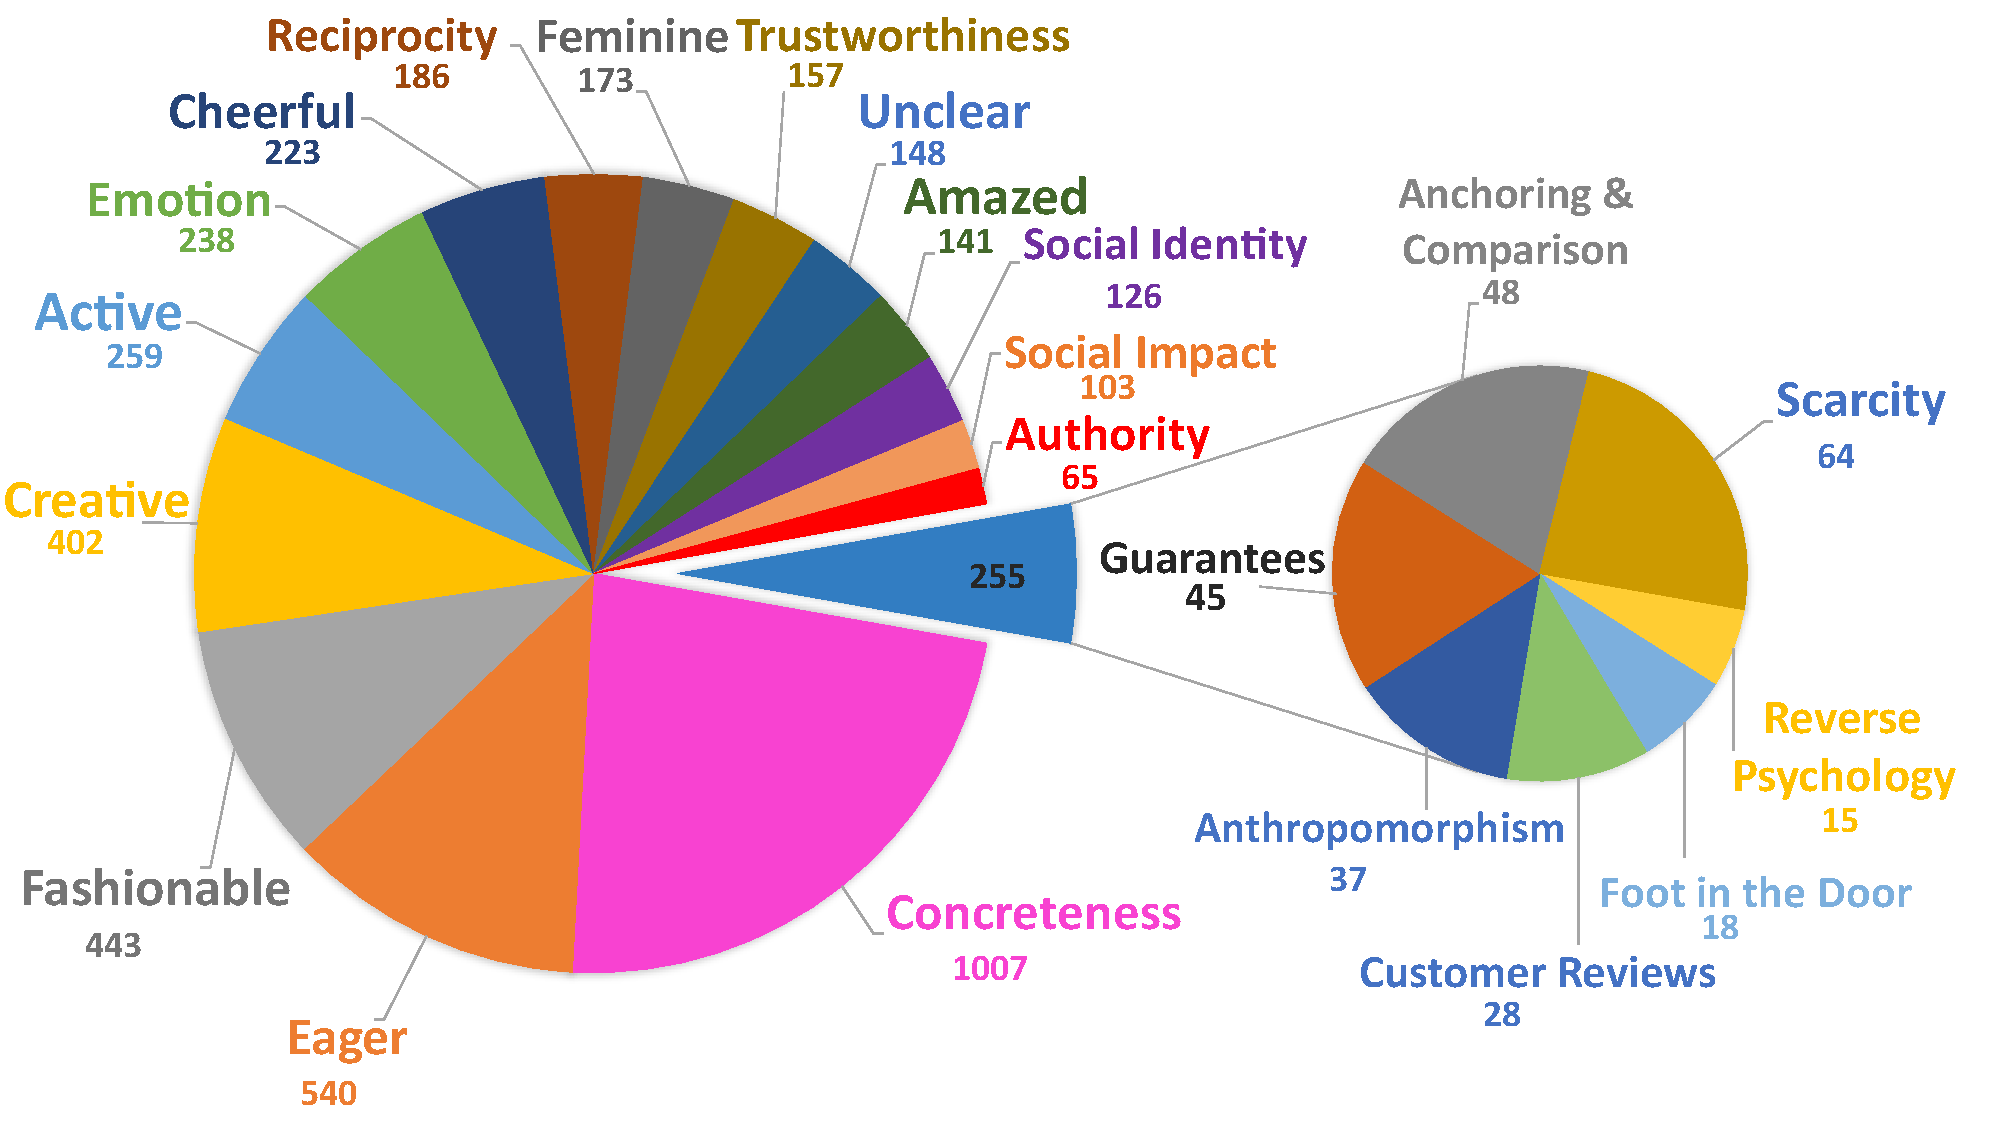
\includegraphics[scale=0.3]{images/pie_chart.pdf}
        \caption{Distribution of Persuasion Strategies in the image persuasion strategy dataset. The top-3 strategies are Concreteness, Eager, and Fashionable. \small}
        \label{fig:persuasion-strategies-distribution}
        % \vspace{-4mm}
    \end{figure}


\subsection{Persuasion Strategy Dataset For Image Advertisements}

To annotate persuasion strategies on image advertisements, we leverage raw images from the Pitts Ads dataset. It contains 64,832 image ads with labels of topics, sentiments, symbolic references (\textit{e.g.} dove symbolizing peace), and reasoning the ad provides to its viewers (see Fig~\ref{fig:preds-sup} for a few examples). The dataset had ads spanning multiple industries, products, services, and also contained public service announcements. Through this, they presented an initial work for the task of understanding visual rhetoric in ads. Since the dataset already had a few types of labels associated with the ad images, we used active learning on a model trained in a multi-task learning fashion over the reasoning task introduced in their paper. We explain the model and then the annotation strategy followed in \S\ref{sec:Persuasion Strategy Prediction Model}. 







To commence training, we initially annotated a batch of $250$ randomly selected ad images with persuasion strategies defined in Section~\ref{tab:persuasive-strategies-list}. We recruited four research assistants to label persuasion strategies for each advertisement. Definitions and examples of different persuasion strategies were provided, together with a training session where we asked annotators to annotate a number of example images and walked them through any disagreed annotations. To assess the reliability of the annotated labels, we then asked them to annotate the same 500 images and computed Cohen's Kappa statistic to measure inter-rater reliability. We obtained an average score of 0.55. The theoretical maximum of Kappa, given the unequal distribution, is 0.76. In such cases, Cohen \cite{cohen1960coefficient} suggested that one should divide kappa by its maximum value $\mathbf{k}/\mathbf{k_{max}}$, which comes out to be 0.72. This is a \textit{substantial} agreement. Further, to maintain labeling consistency, each image was double annotated, with all discrepancies resolved by an intervention of the third annotator using a majority vote. 


The assistants were asked to label each image with no more than 3 strategies. If an image had more than 3 strategies, they were asked to list the top 3 strategies according to the area covered by the pixels depicting that strategy. In total, we label 3000 ad-images with their persuasion strategies; and the number of samples in train, val, and test split are 2500, 250, and 250, respectively\footnote{Table~\ref{table:strategy-train-test-val-stats} shows the detailed distribution of the number of strategies in ads}. Fig.~\ref{fig:persuasion-strategies-distribution} presents the distribution of persuasion strategies in the dataset. It is observed that concreteness is the most used strategy in the dataset, followed by eagerness and fashion. The average number of strategies in an ad is 1.49, and the standard deviation is 0.592. We find that scarcity (92.2\%), guarantees (91.1\%), reciprocity (84.4\%), social identity (83.3\%), and cheerful (83\%), %and anchoring and comparison (77.1\%), trustworthiness (75.8\%), social proof (75\%),  amazed (73.1\%) and concreteness (70.3\%) 
are the top 5 strategies, which occur in groups of 2 or 3. We observe that the co-occurrence of these strategies is due to the fact that many of them cover only a single modality (\textit{i.e.}, text or visual), leaving the other modality free for a different strategy. For example, concreteness is often indicated by illustrating points in text, while the visual modality is free for depicting, say, emotion. See Fig.~\ref{fig:segmented image} for an example, where the image depicting \textit{Authority} also has concreteness strategy in it. Similarly, feminine emotion is also depicted in Fig.~\ref{fig:footwear-strategies}, along with concreteness.


\begin{figure*}[!h]
    % \vspace{-4mm}
    \centering
    \begin{subfigure}[b]{0.4\textwidth}
        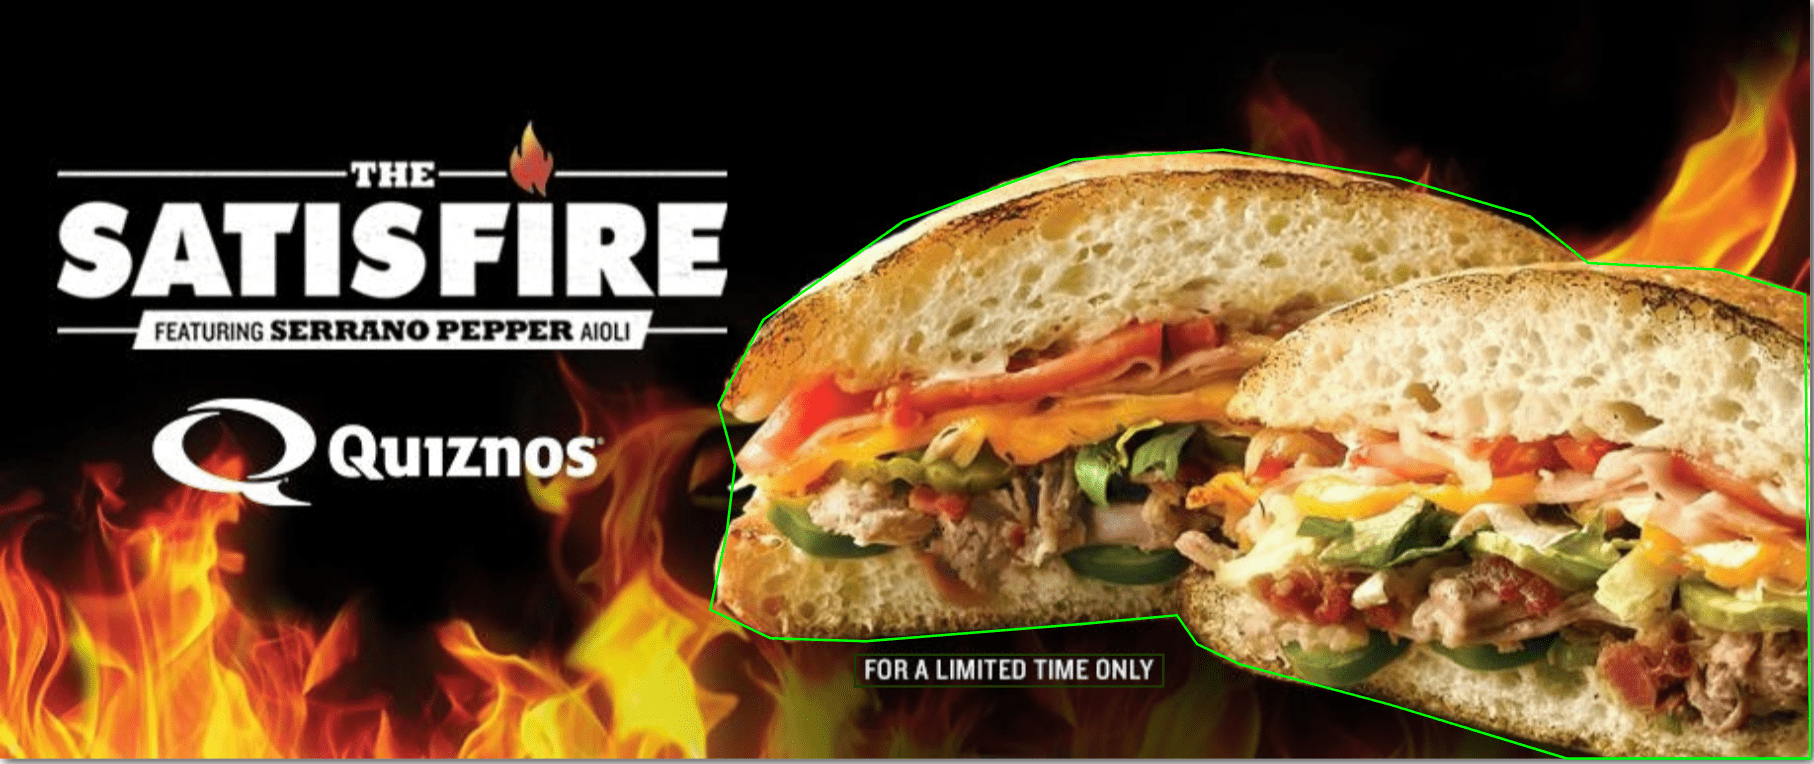
\includegraphics[scale=0.2]{images/Image1.png}
    \end{subfigure}
    \begin{subfigure}[b]{0.4\textwidth}
        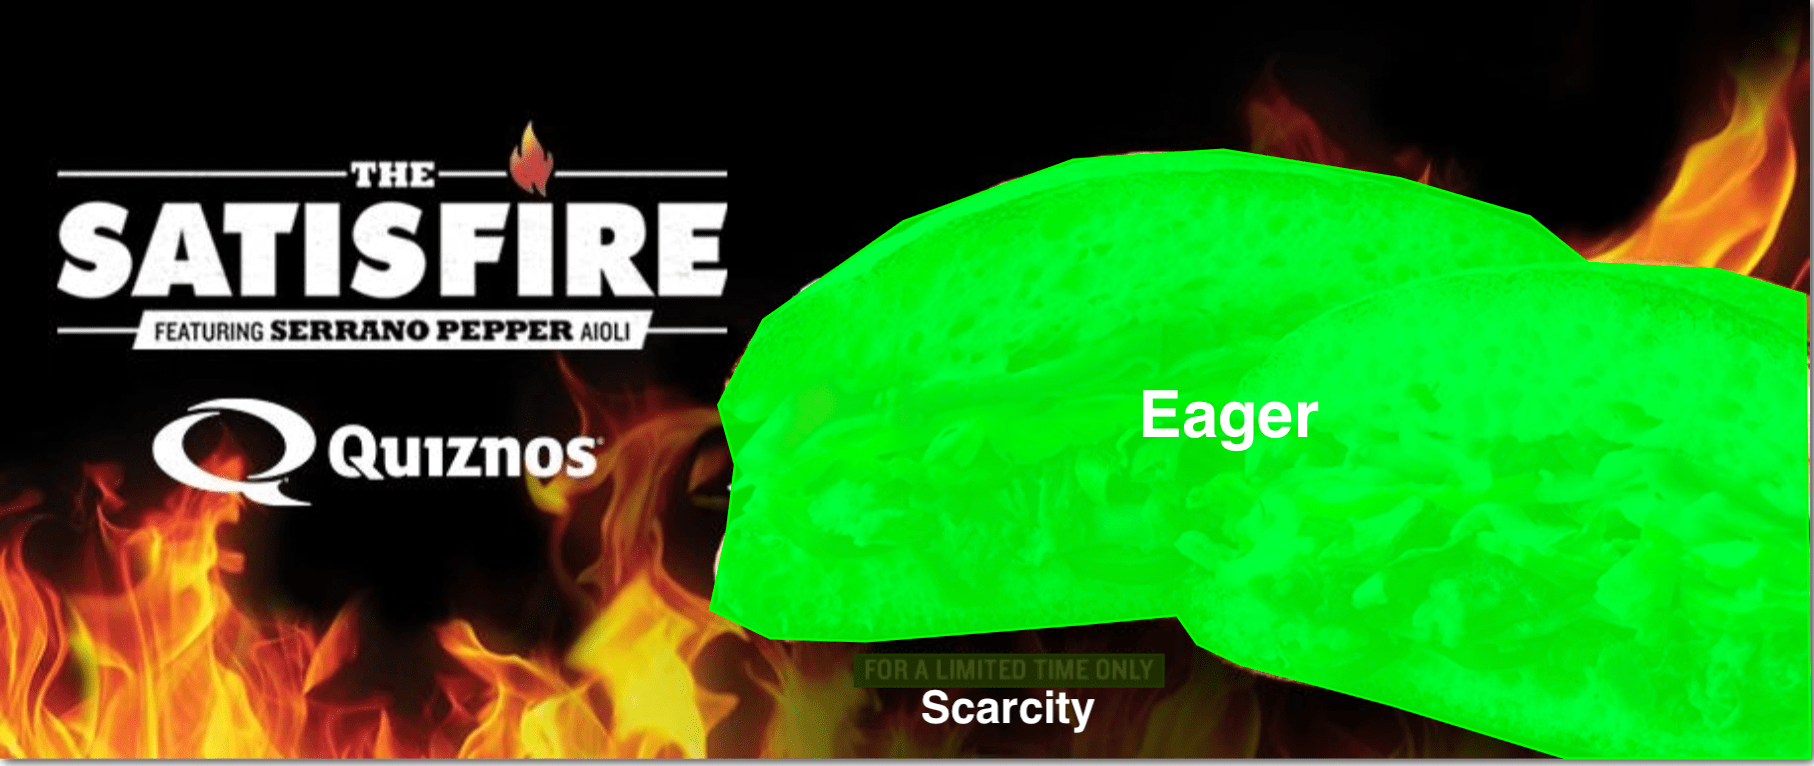
\includegraphics[scale=0.2]{images/Image1_Segment.png}



    \end{subfigure}
     \begin{subfigure}[b]{0.245\textwidth}
         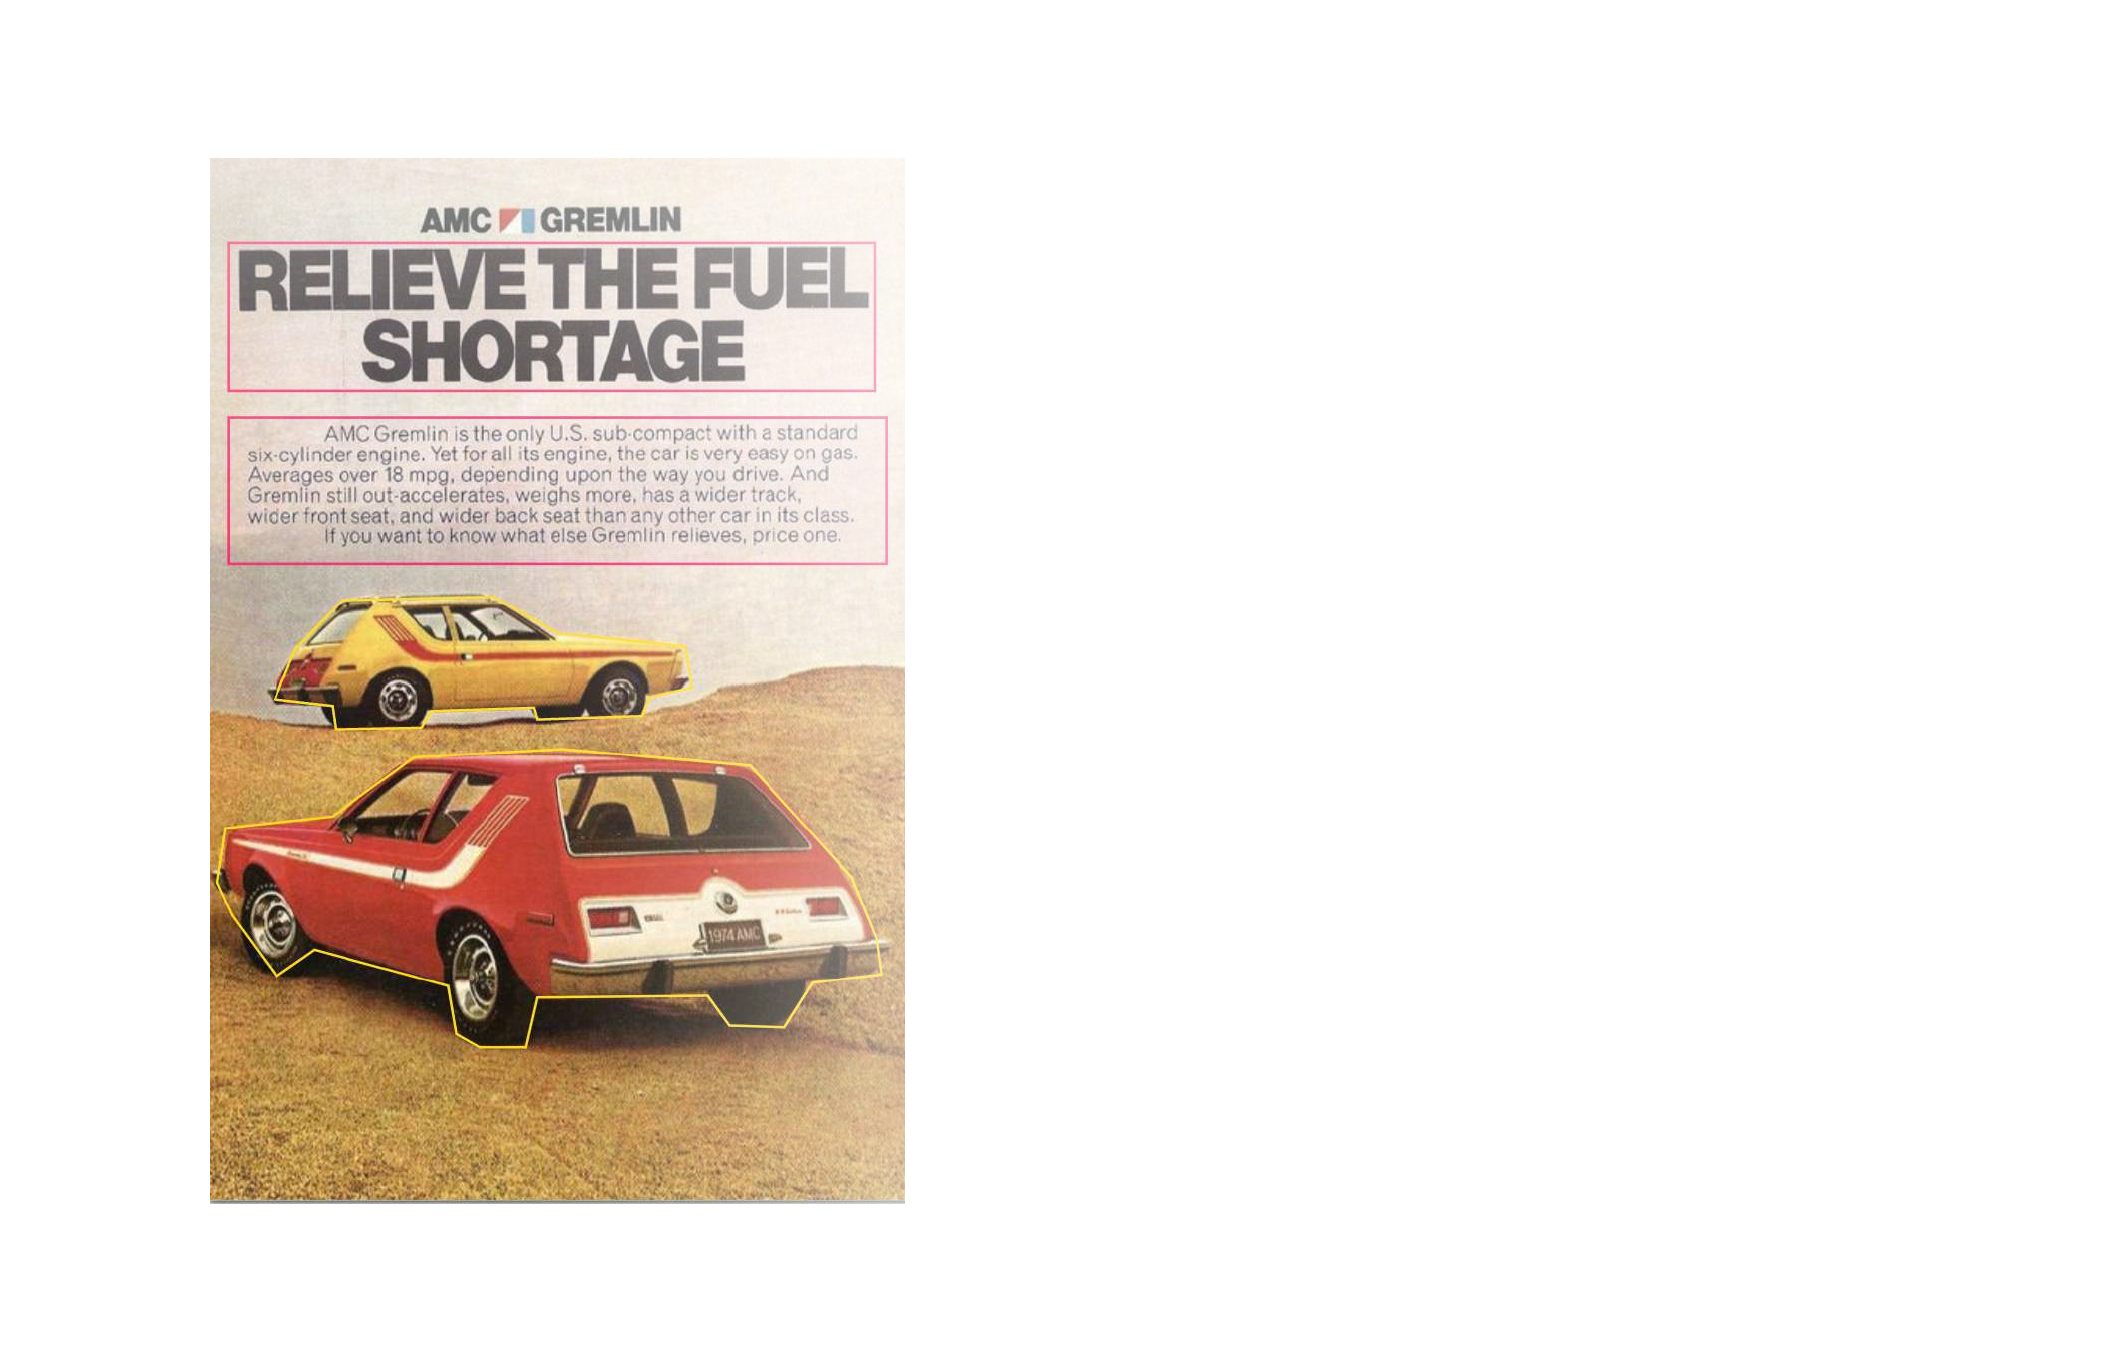
\includegraphics[scale=0.22]{images/fuel-shortage-original.pdf}
     \end{subfigure}
     \begin{subfigure}[b]{0.245\textwidth}
         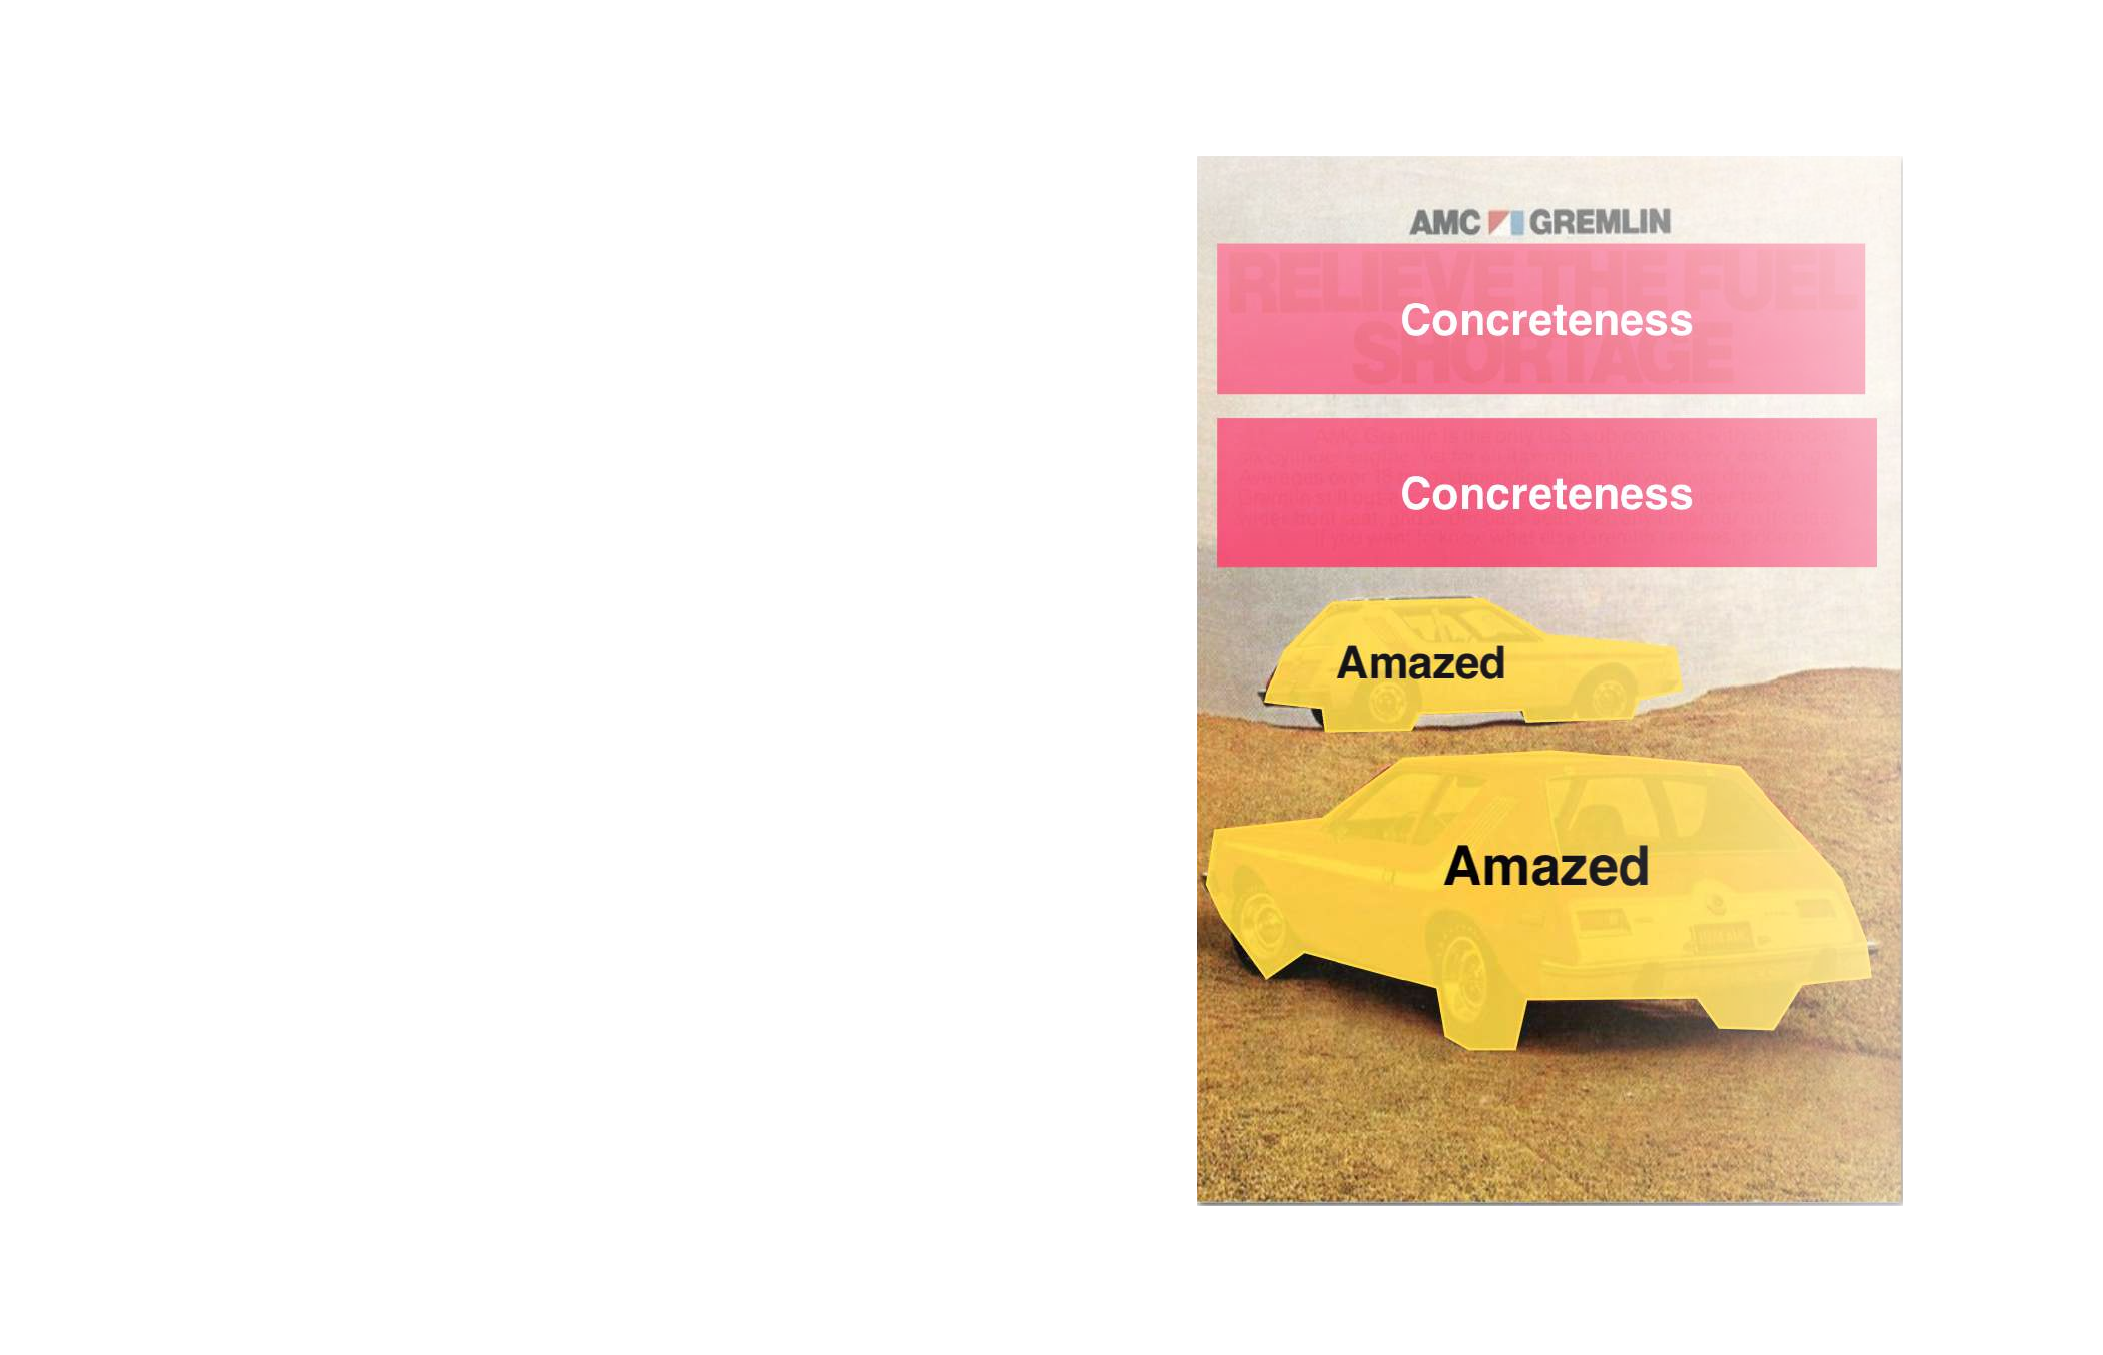
\includegraphics[scale=0.22]{images/fuel-shortage-segmented.pdf}
     \end{subfigure}
     \begin{subfigure}[b]{0.24\textwidth}
         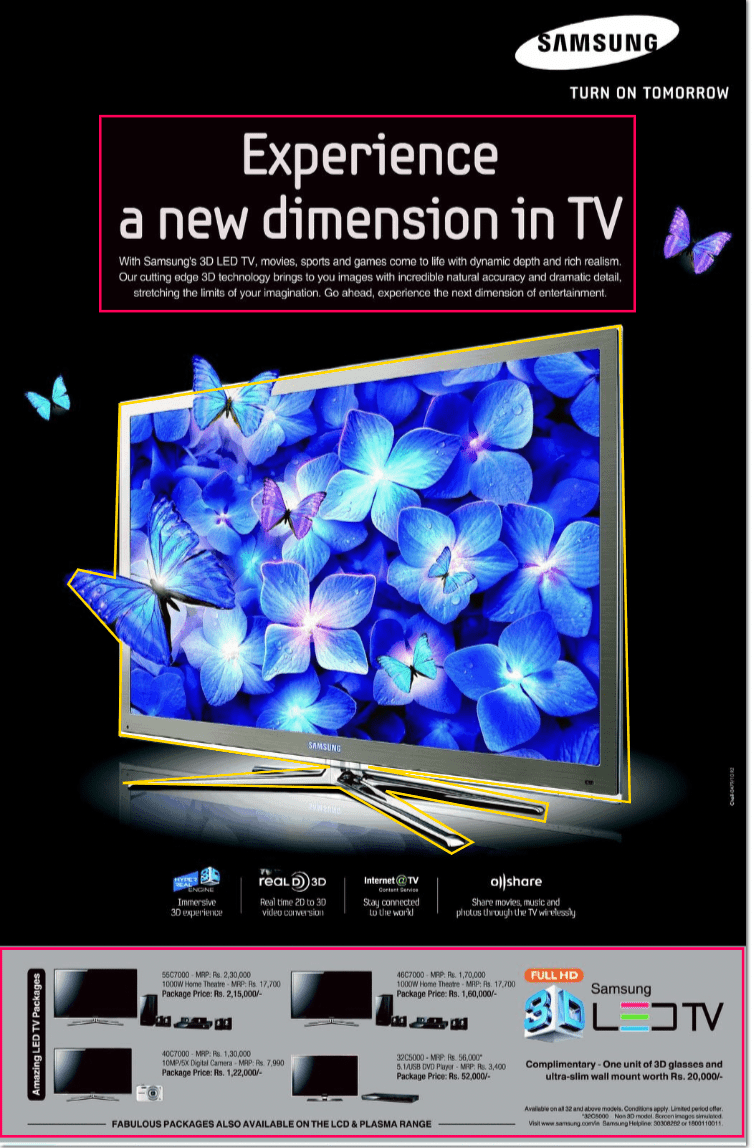
\includegraphics[scale=0.22]{images/Image2.png}
     \end{subfigure}
     \begin{subfigure}[b]{0.24\textwidth}
         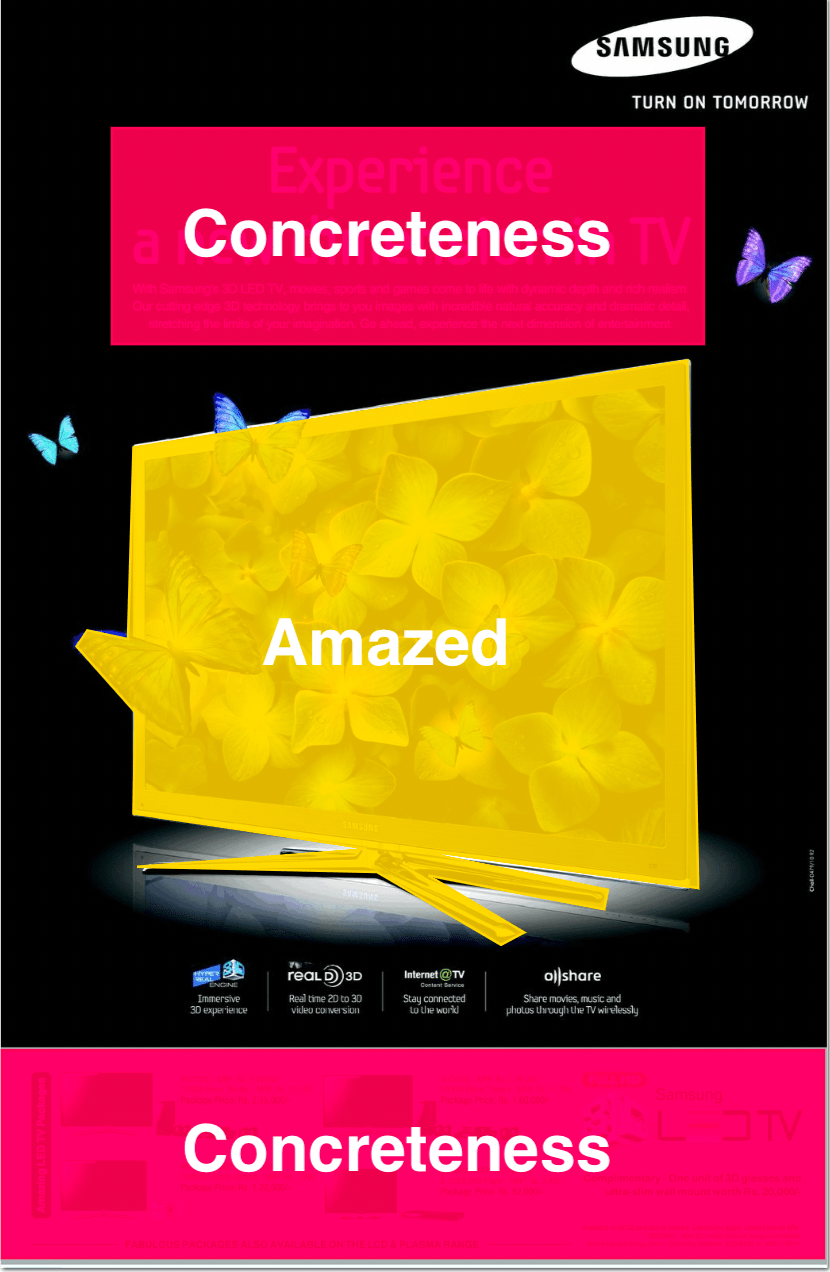
\includegraphics[scale=0.22]{images/Image2_Segment.png}
     \end{subfigure}


    \begin{subfigure}[b]{0.24\textwidth}
        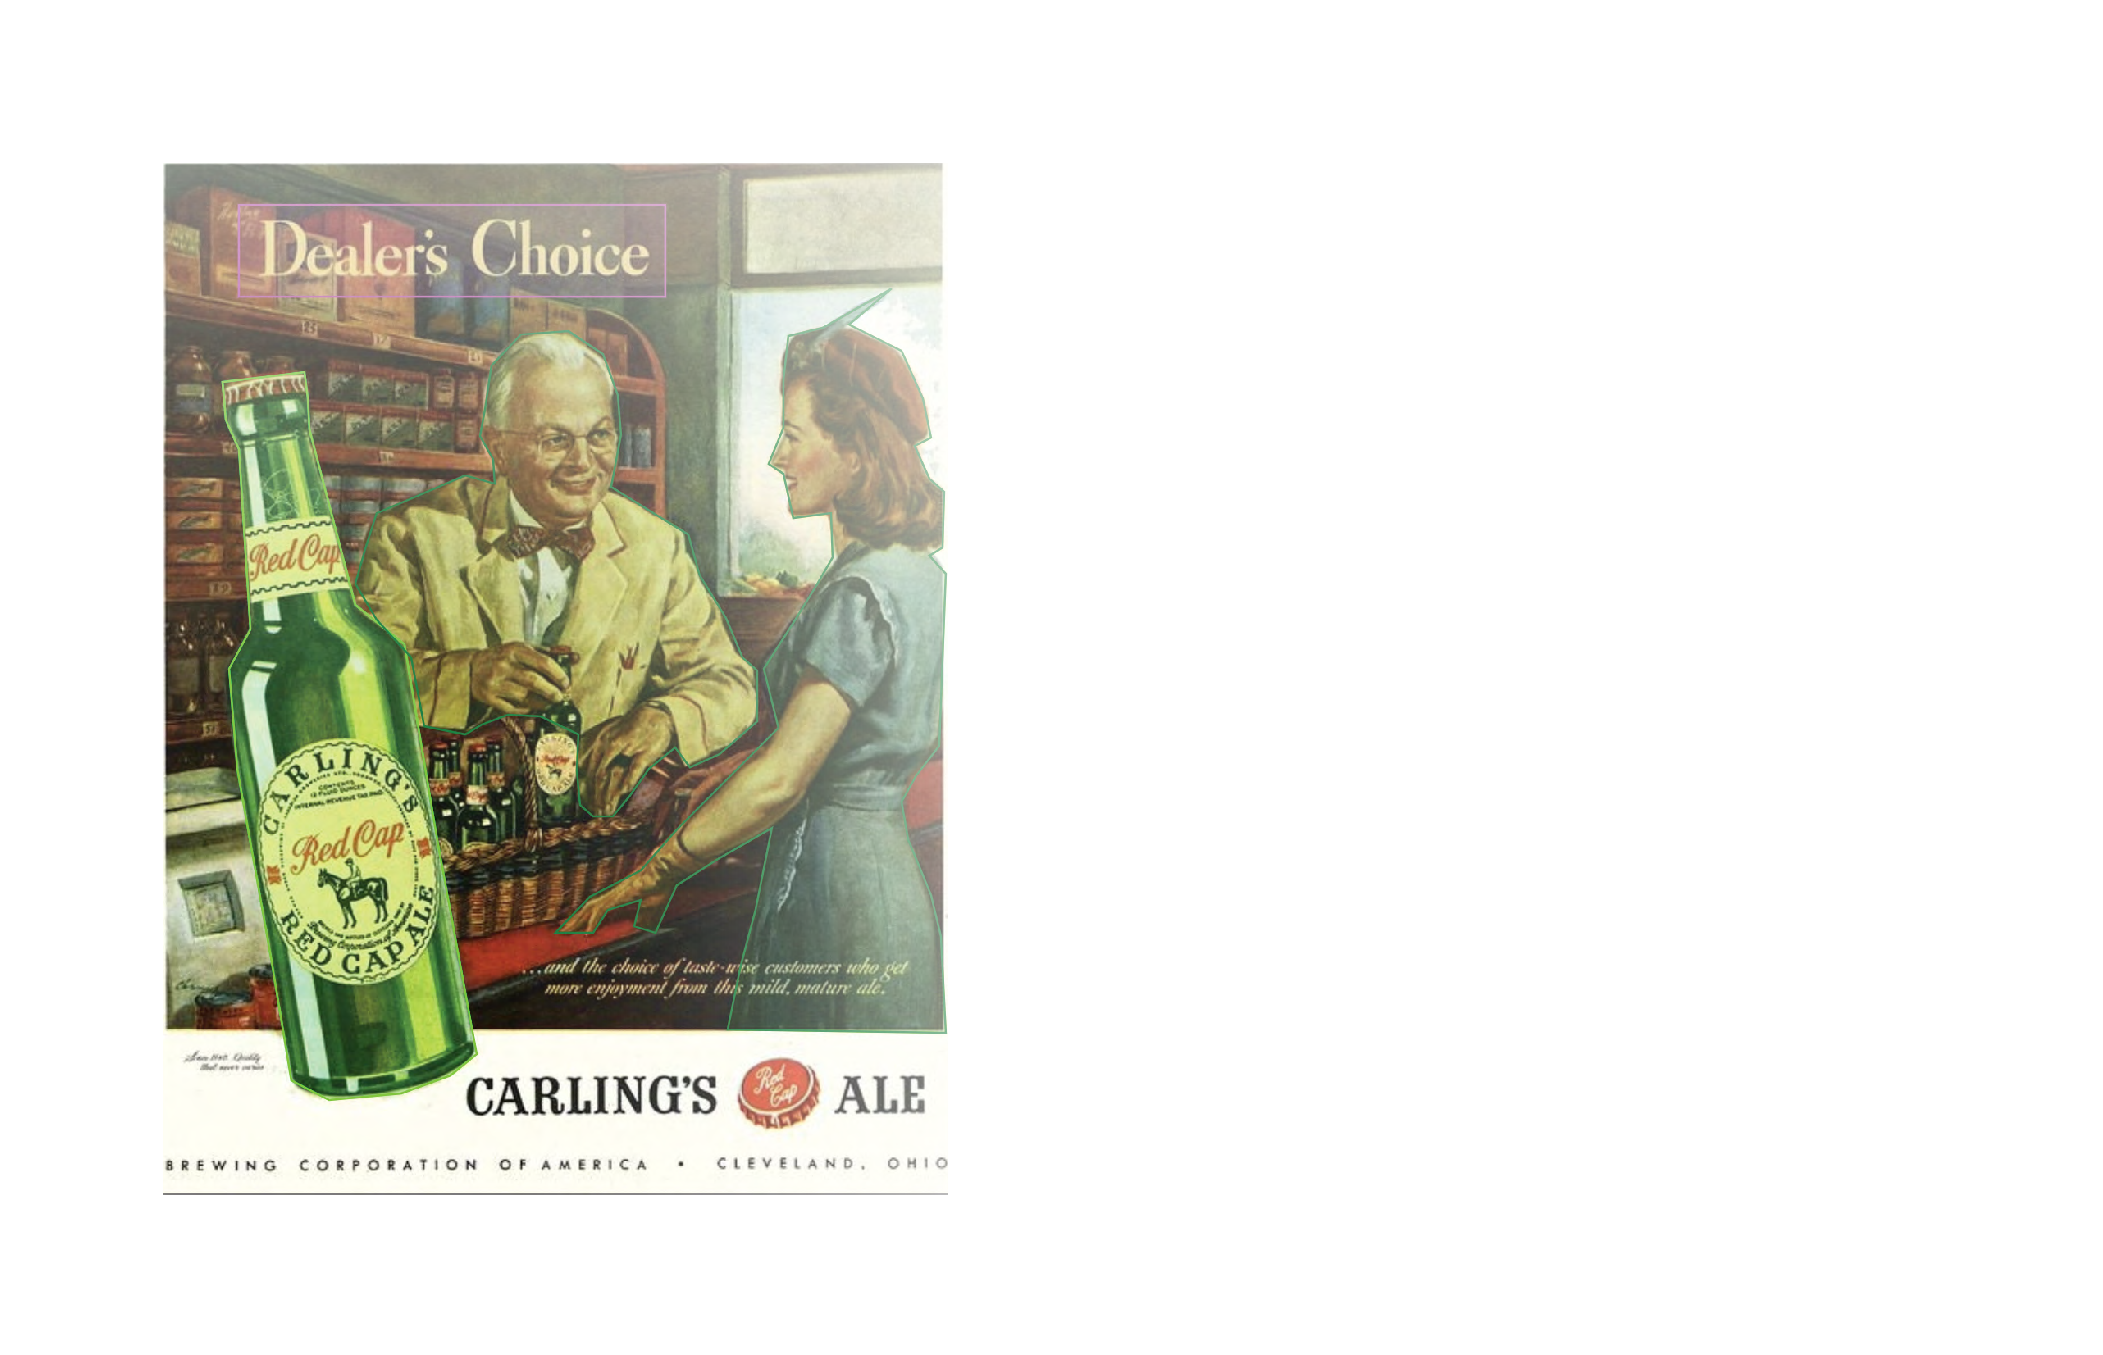
\includegraphics[scale=0.22]{images/dealer-choice-original.pdf}
    \end{subfigure}
    \begin{subfigure}[b]{0.24\textwidth}
        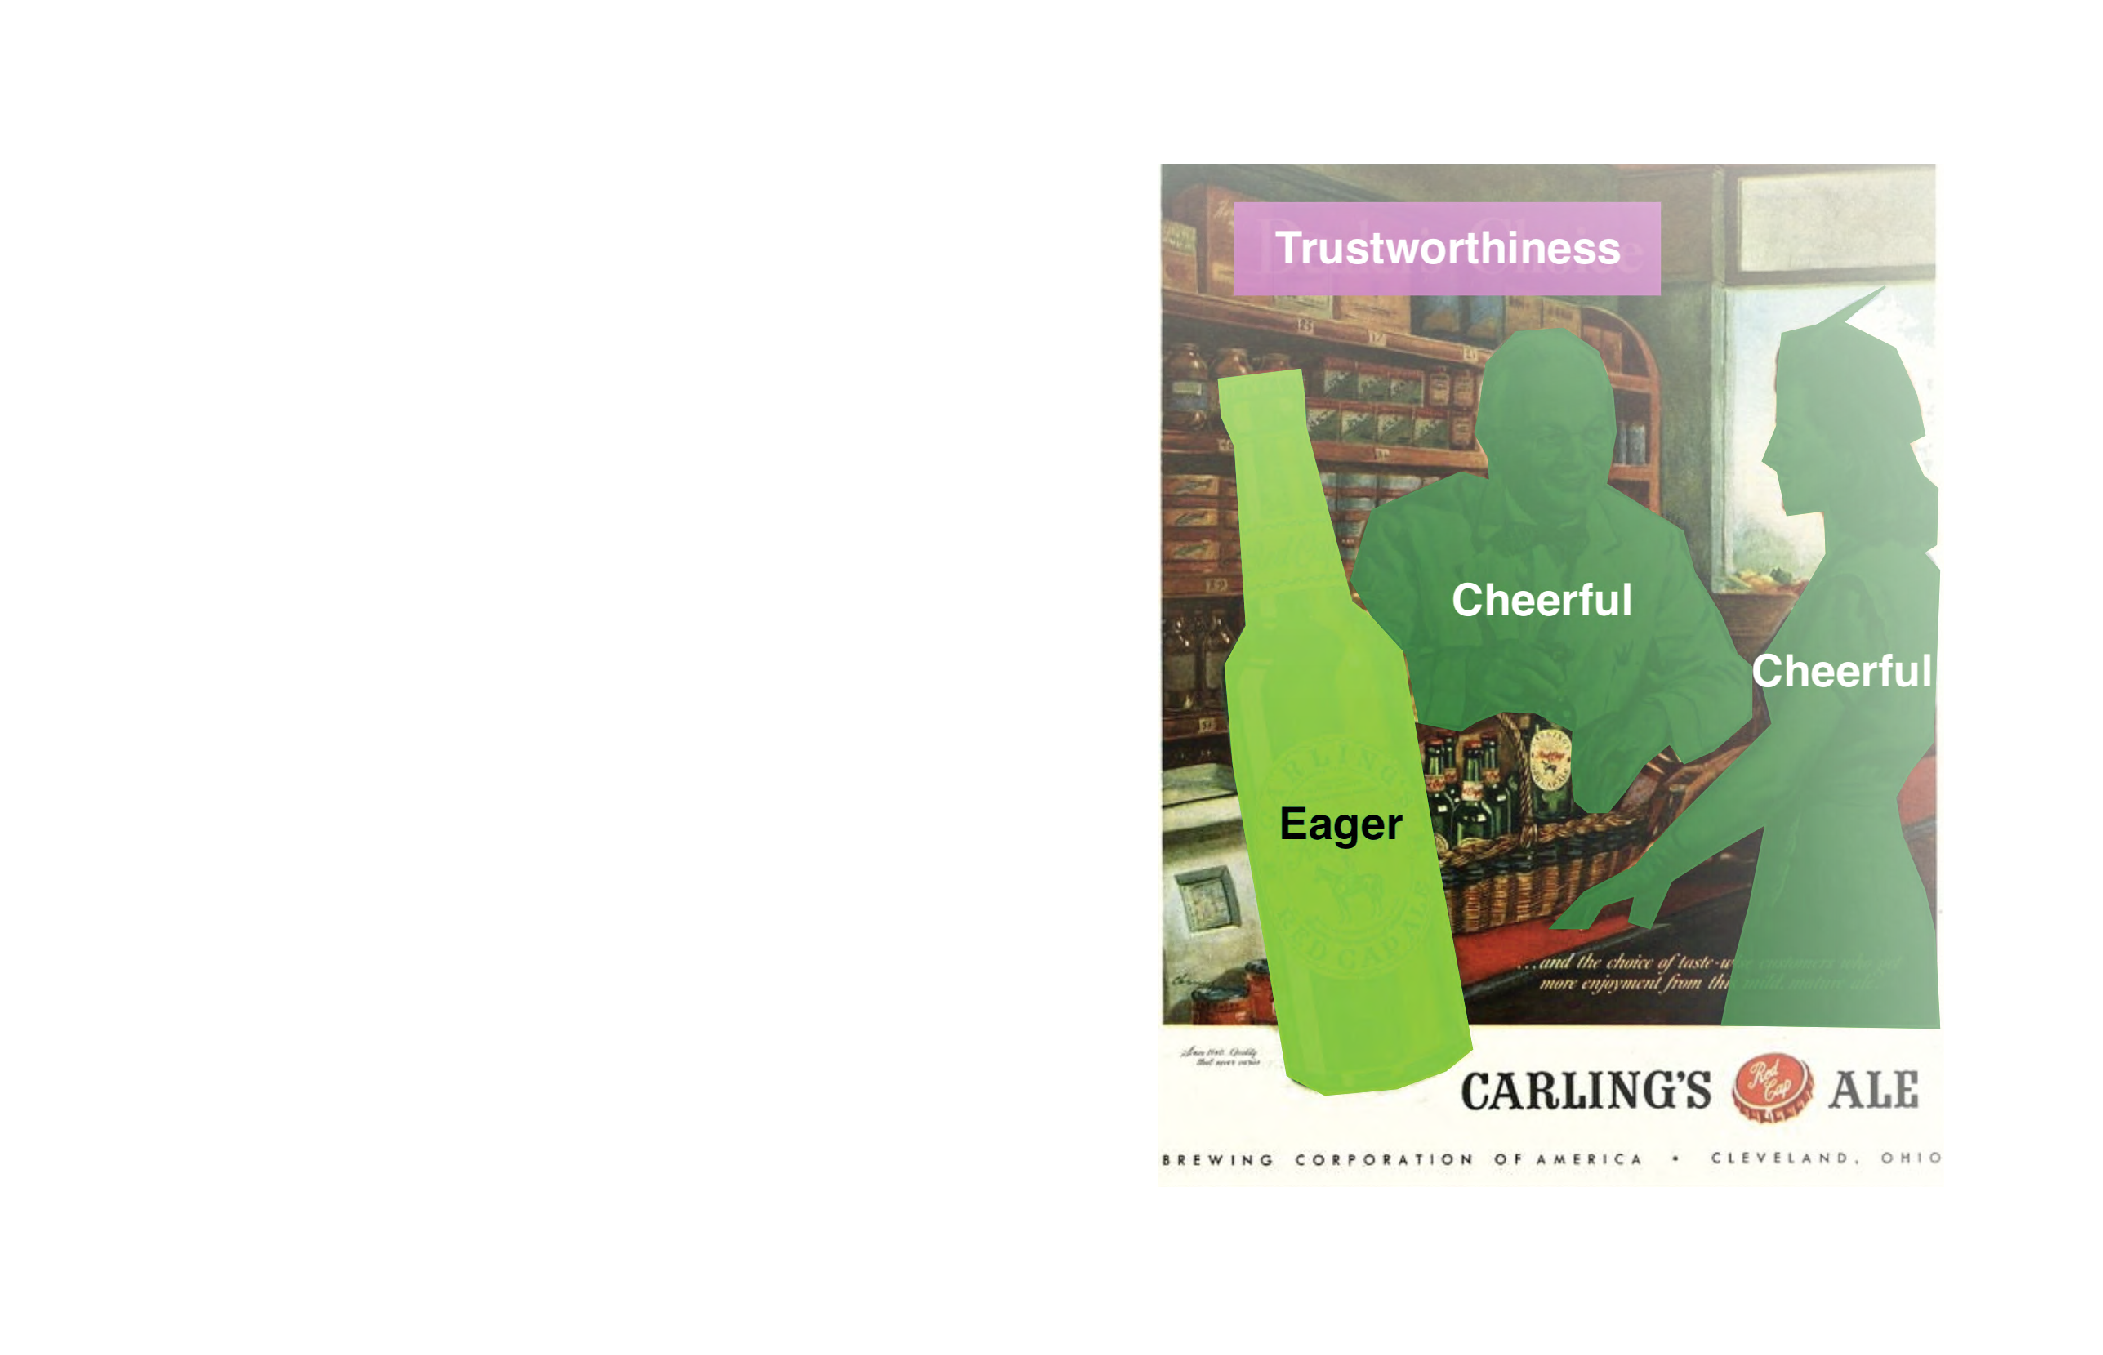
\includegraphics[scale=0.22]{images/dealer-choice-segmented.pdf}
    \end{subfigure}
     \begin{subfigure}[b]{0.24\textwidth}
         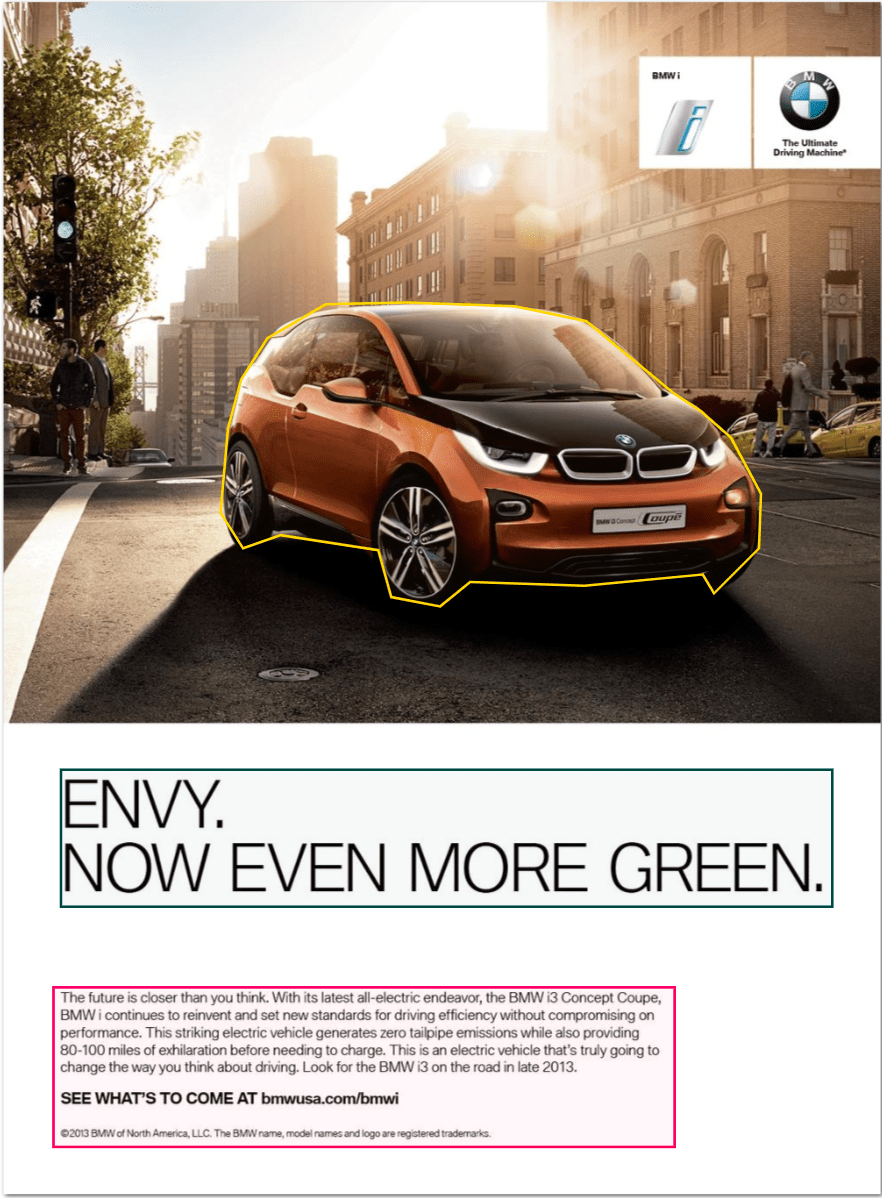
\includegraphics[scale=0.22]{images/Image3.png}
     \end{subfigure}
     \begin{subfigure}[b]{0.24\textwidth}
         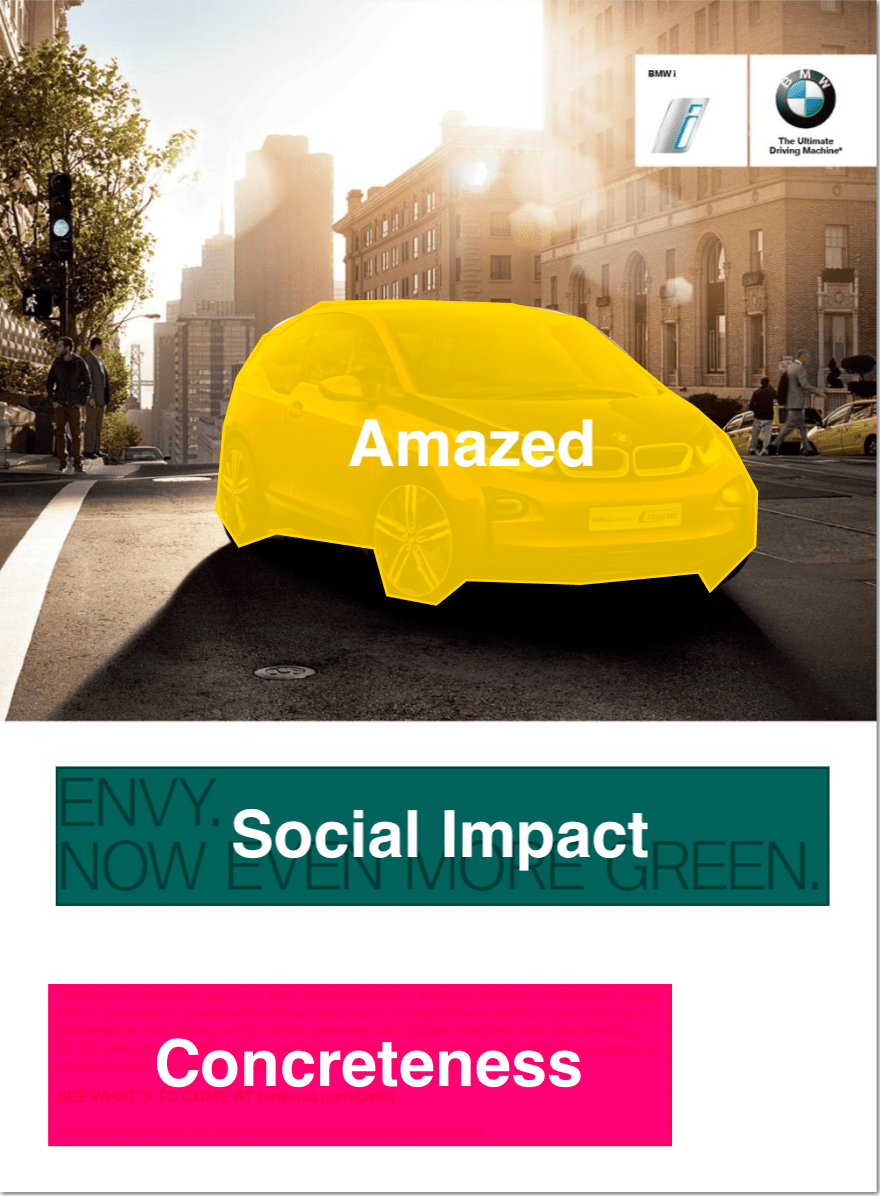
\includegraphics[scale=0.22]{images/Image3_Segment.png}
     \end{subfigure}
     
     \begin{subfigure}[b]{0.4\textwidth}
         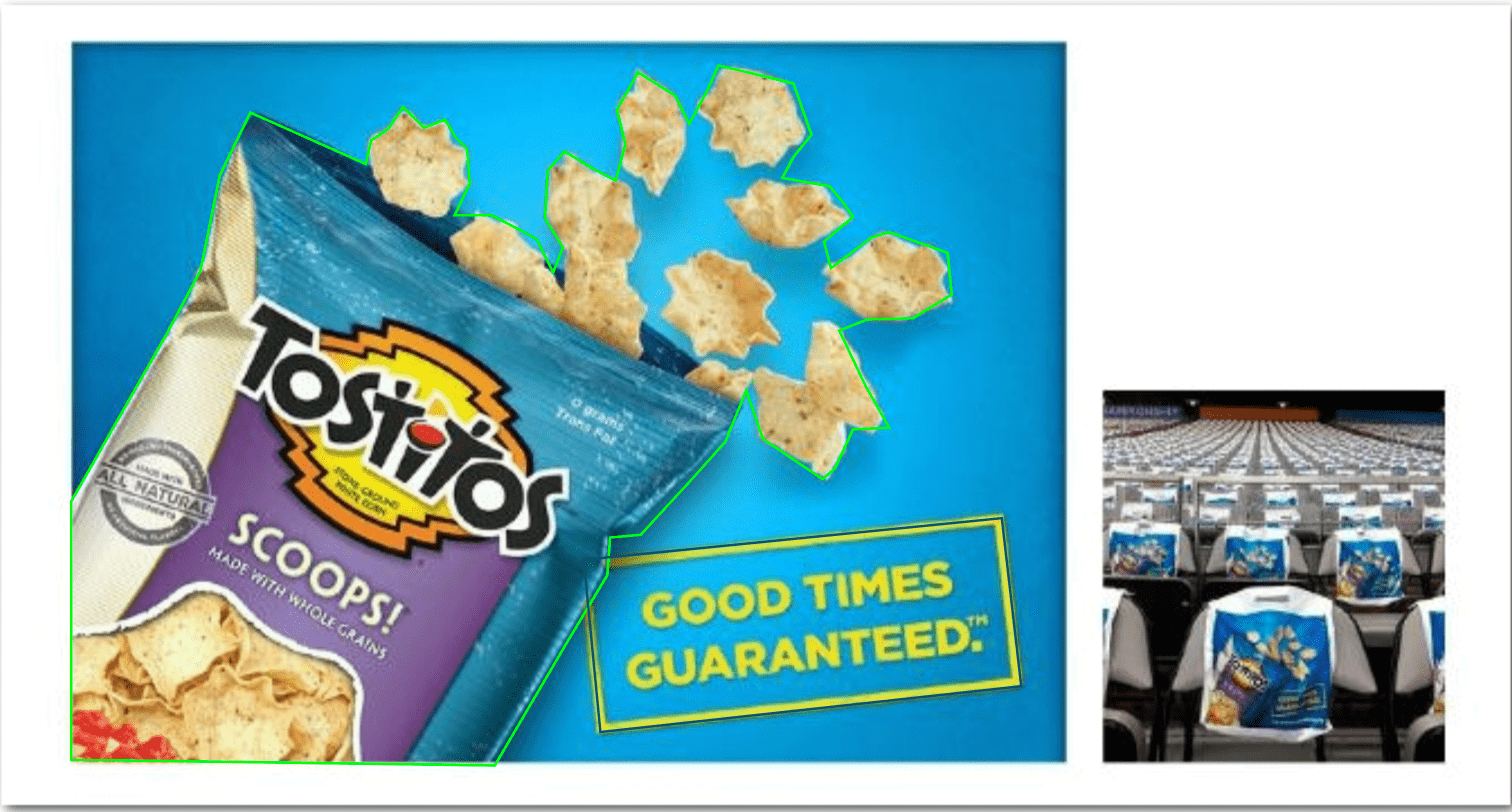
\includegraphics[scale=0.22]{images/Image4.png}
     \end{subfigure}
     \begin{subfigure}[b]{0.4\textwidth}
         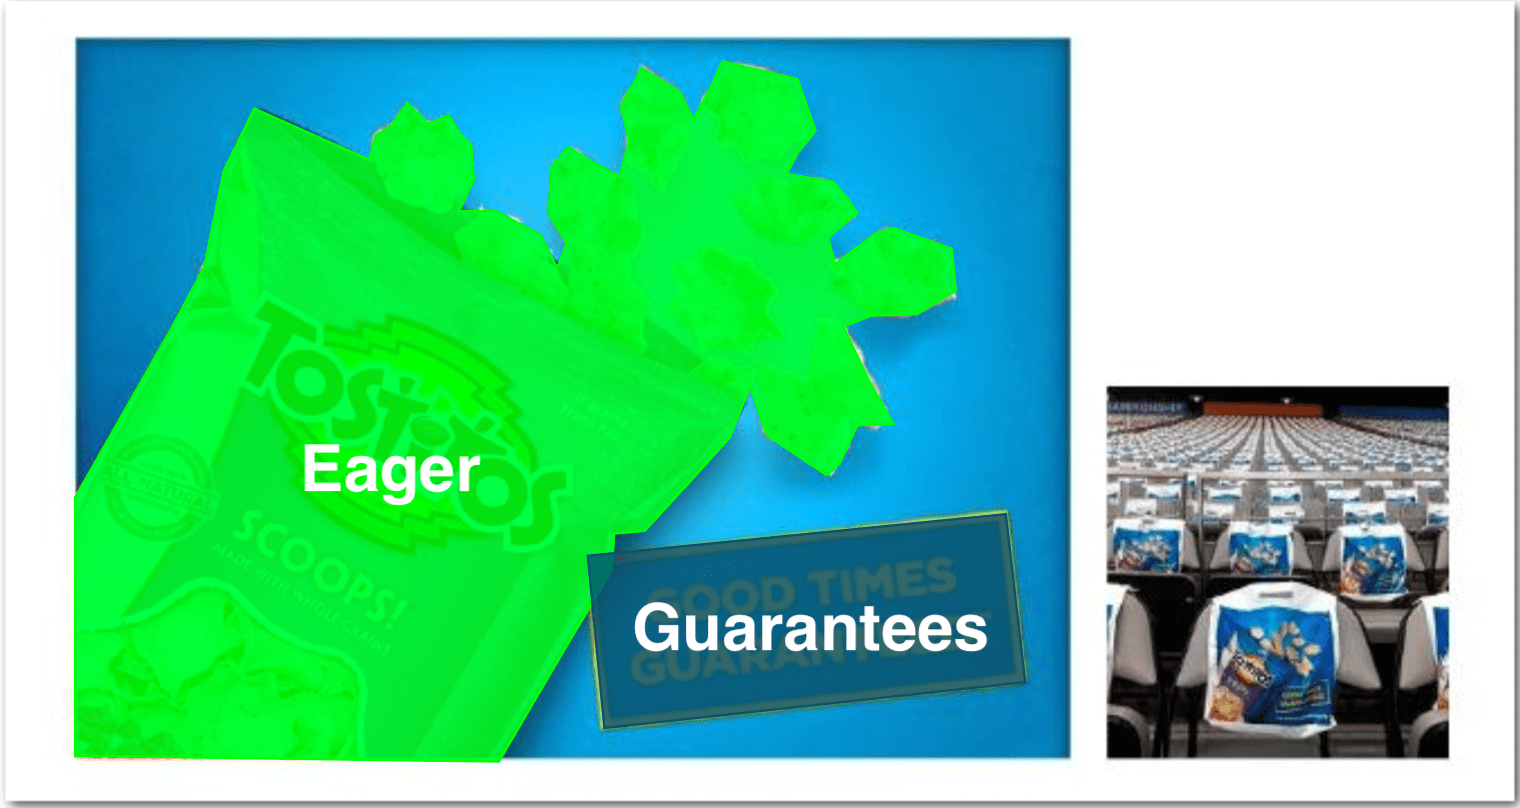
\includegraphics[scale=0.22]{images/Image4_Segment.png}
     \end{subfigure}
     
    \caption{\small \label{fig:segmented image} Image with a segmentation mask depicting the strategies \textit{Emotion:Cheerful}, \textit{Emotion:Eager} and \textit{Trustworthiness}.}
    % \vspace{-4mm}
\end{figure*}







Next, we calculate the Dice correlation coefficient\footnote{The Dice Coefficient is defined as: \; \(2*|X \cap Y|\: / \:(|X|+|Y|)\), where X and Y are two sets; a set with vertical bars on either side refers to the cardinality of the set, i.e. the number of elements in that set; and \(\cap\)  refers to the intersection of two sets.} statistics for pairs of co-occurring persuasion strategies. The top-5 pairs are eager-concreteness (0.27), scarcity-reciprocity (0.25), eager-cheerful (0.19), amazed-concreteness (0.17), and eager-reciprocity (0.17). We find that these correlation values are not particularly high since marketers seldom use \textit{common pairings} of messaging strategies to market their products. The visual part mostly shows eager strategy in ads; therefore, we find that the text modality becomes free to show other strategies. That is why primarily text-based concreteness, cheerfulness, and reciprocity strategies are present with the visual-based eager strategy in the text modality. Also, primarily vision-based amazement, eagerness, and scarcity (short-text) strategies co-occur with text-based reciprocity and concreteness (\textit{e.g.}, Fig.~\ref{fig:footwear-strategies}).


\begin{figure*}
    \centering
    \begin{subfigure}[b]{0.3\textwidth}
         \centering
         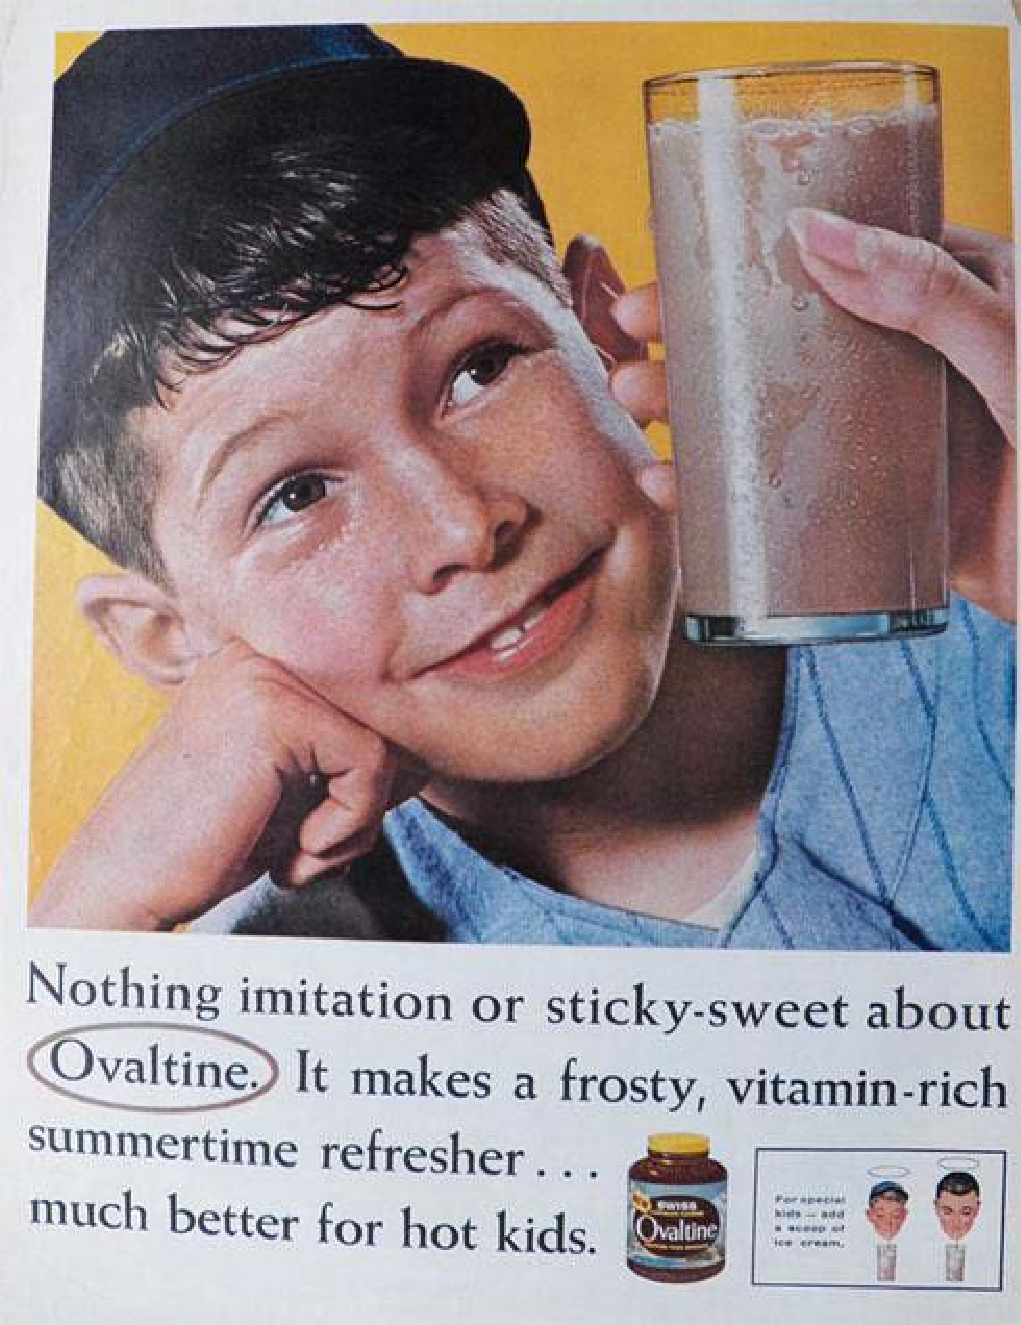
\includegraphics[width=\textwidth,scale=0.6]{images/humans_concreteness_img1.pdf}
         \caption{}
         
     \end{subfigure}
     \begin{subfigure}[b]{0.3\textwidth}
         \centering
         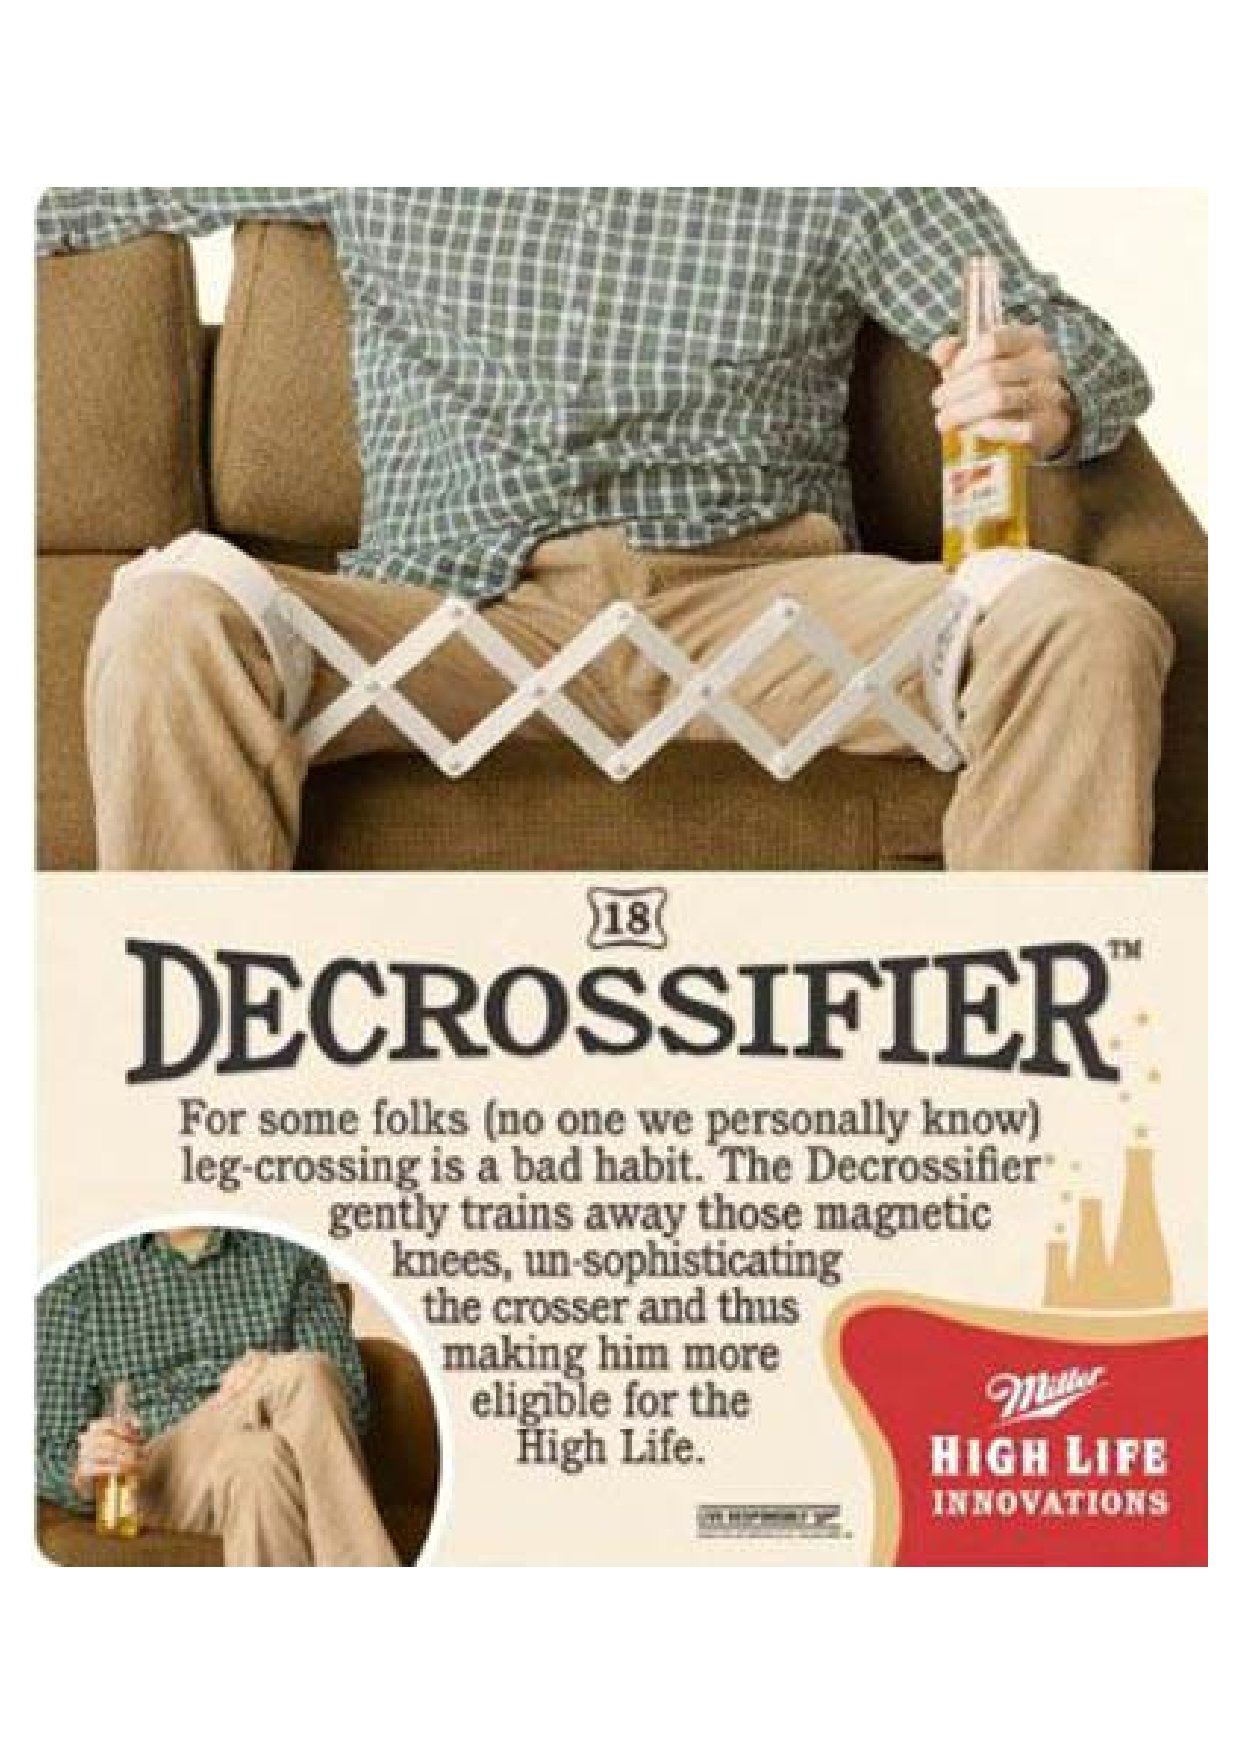
\includegraphics[width=\textwidth,scale=0.5]{images/humans_concreteness_img2.pdf}
         \caption{}
         
     \end{subfigure}
     \begin{subfigure}[b]{0.3\textwidth}
         \centering
         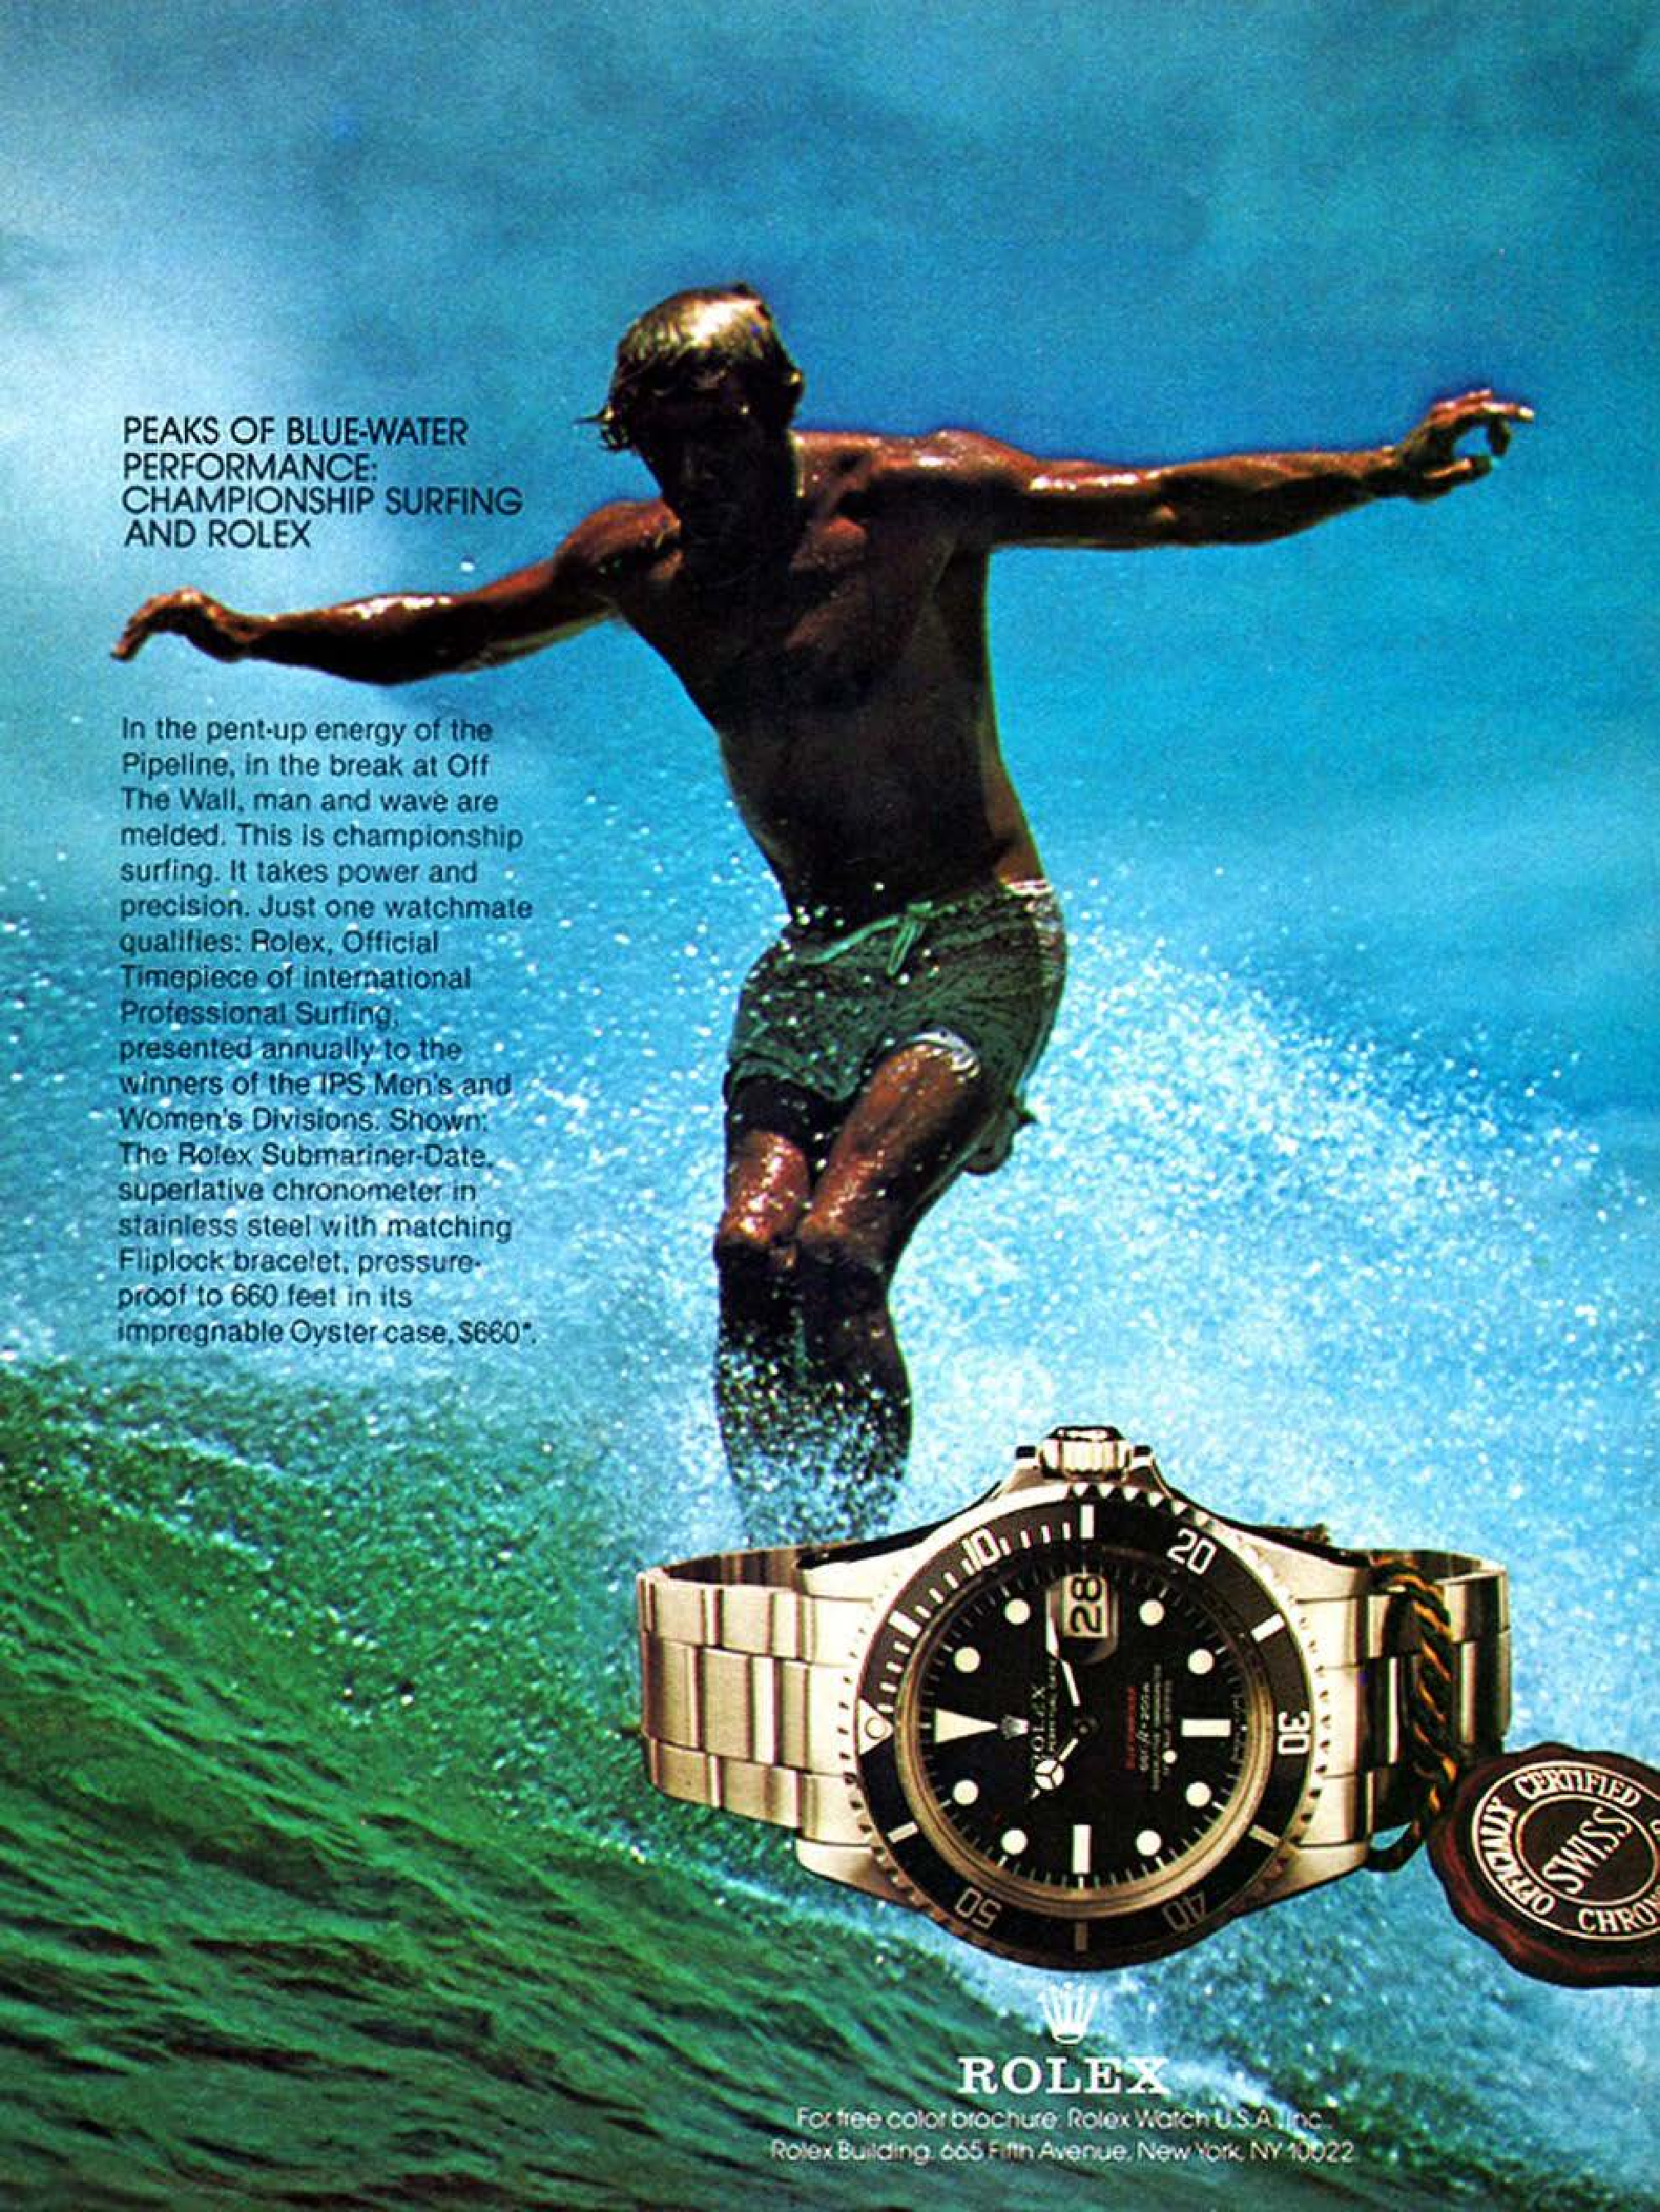
\includegraphics[width=\textwidth,scale=1.0]{images/humans_concreteness_img3.pdf}
         \caption{}
         
     \end{subfigure}
    \caption{Advertisements containing humans and concreteness}
    \label{fig:humans_concreteness-ads}
\end{figure*}




\begin{figure}[h]
        \centering
        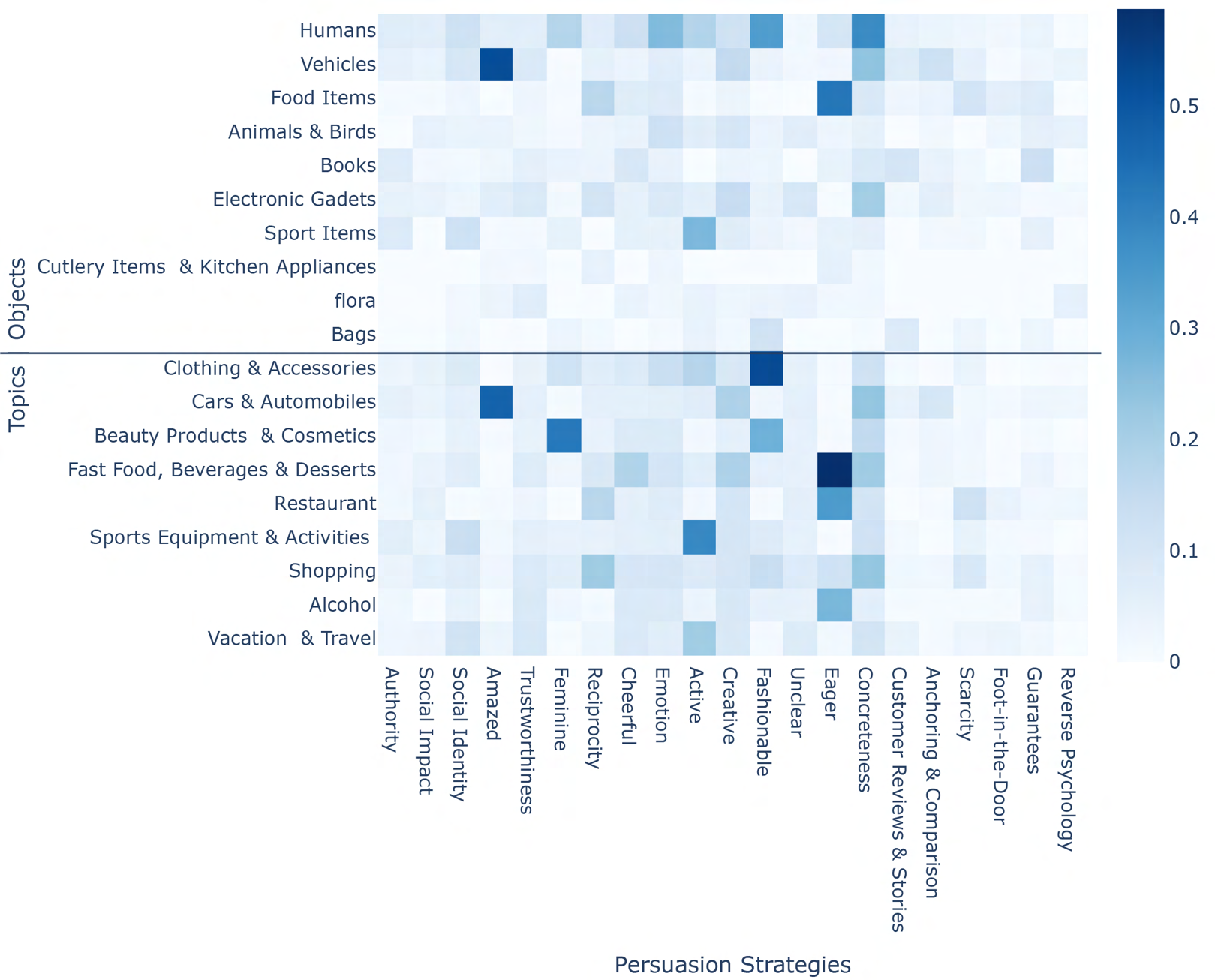
\includegraphics[scale=0.55]{images/objects_topics.pdf}
        \caption{Dice correlation between topics and strategies. Topics are taken from the Pitts Ad dataset and further similar topics are combined to get these values.}
        \label{fig:correlation-between-topics-and-strategies}
        % \vspace*{-3mm}
    \end{figure}

Next, we calculate the correlation between image topics and objects present with persuasion strategies. We see that the emotion:feminine and emotion:fashionable strategies are most often associated with beauty products and cosmetics (corr=0.4256, 0.2891). This is understandable since most beauty products are aimed at women. We see that the fast-food and restaurant industries often use eagerness as their messaging strategy (corr = 0.5877,0.3470). We find that the presence of humans in ads is correlated with the concreteness strategy (see Fig~\ref{fig:humans_concreteness-ads} for a few examples) (corr=0.3831). On the other hand, vehicle ads use emotion:amazed and concreteness (corr=0.5211,0.2412) (see Fig:\ref{fig:correlation-between-topics-and-strategies} for detailed correlations). 

Similar to a low correlation in co-occurring strategies, we find that product segments and their strategies are not highly correlated. This is because marketers use different strategies to market their products even within a product segment. Fig.~\ref{fig:footwear-strategies} shows an example in which the footwear industry (which is a subsegment of the apparel industry) uses different strategies to market its products. Further, for a batch of $250$ images, we also label segmented image regions corresponding to the strategies present in the image. These segment masks were also double-annotated. Fig.~\ref{fig:segmented image} presents an example of masks depicting parts of the image masked with different persuasion strategies in a drink advertisement.





\subsection{Persuasion Strategy Dataset For Video Advertisements}
For this task, we collected 2203 video advertisements from popular brands publicly available on the web. We use the following 12 strategies as our target persuasion strategy set: \textit{Social Identity, Concreteness, Anchoring and Comparison, Overcoming Reactance, Reciprocity, Foot-in-the-Door, Authority, Social Impact, Anthropomorphism, Scarcity, Social Proof,} and \textit{Unclear}. We use non-experts human annotators to label this dataset (as compared to expert humans for the image ads dataset). In order to make the class labels easier to understand for non-expert human annotators, we make a list of 15 yes/no type-questions containing questions like ``\textit{Was there any expert (person or company) (not celebrity) encouraging to use the product/brand? Was the company showcasing any awards (e.g., industrial or government)? Did the video show any customer reviews or testimonials?}'' (complete list in Table~\ref{table:persuasion strategy questions}). 

Each human annotator watches 15 videos such that each video gets viewed by at least two annotators and answers these questions for each video. Based on all the responses for a video, we assign labels to that video. We remove videos with an inter-annotator score of less than 60\%. After removing those, we get a dataset with 1002 videos, with an average length of 33 secs and a distribution as shown in Fig.~\ref{fig:persuasion-strategy-dataset-distribution}. This dataset is then used for the persuasion strategy identification task. 


\begin{figure}[!h]
    \centering
    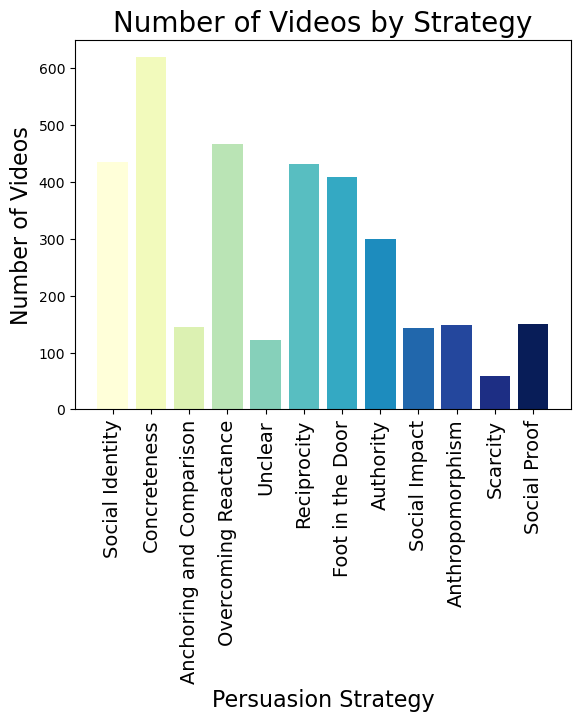
\includegraphics[width=0.5\textwidth]{images/video_strategies.png}
    \caption{Distribution of persuasion strategies in our video persuasion strategy dataset}
    \label{fig:persuasion-strategy-dataset-distribution}
\end{figure}


\begin{table*}[!hp]
  \centering
  \begin{tabular}{|p{3.5cm}|p{2.3cm}|p{3.5cm}|p{2.3cm}|}
    \hline
    \textbf{Question} & \textbf{Strategy} & \textbf{Question} & \textbf{Strategy} \\
    \hline
    Was there any expert (person or company) (not celebrity) encouraging to use the product/brand? & Authority & Did the video show any normal customers (non-expert, non-celebrity) using the product? & Social Identity \\
    \hline
    Did the video showcase any awards or long usage history of the product/brand? & Authority & Did the video show any customer reviews or testimonials? & Social Proof \\
    \hline
    Was the product/brand comparing itself with other competitors or existing solutions? & Anchoring and Comparison & Were any number/statistics mentioned? & Concreteness \\
    \hline
    Did the video talk about any specific features or provide information about the product/brand? & Concreteness & Were there any mention of any offers on the brand/product? & Reciprocity \\
    \hline
    Were the offers limited or available for a short period of time? & Scarcity & Was the product/brand told to be free or available on a discount? & Foot in the Door, Reciprocity \\
    \hline
    Was the brand/product described as simple, easy to use, or can start using with minimal resistance? & Overcoming Reactance, Foot in the Door & Was the brand/product talking about bigger societal impact? & Social Impact \\
    \hline
    Did the brand provide any guarantees that might help reduce the risk of people trying out the product? & Overcoming Reactance & Did the video provide any resources, tips, guides, or tools related to the product? & Reciprocity \\
    \hline
    Is the brand or product portrayed as human-like? & \makecell{Anthropo-\\morphism} & & \\
    \hline
  \end{tabular}
  \caption{The questions we asked to the non-expert annotators to help them identify persuasion strategy contained in the video advertisement. \label{table:persuasion strategy questions}}
\end{table*}





% \vspace{-2mm}
\section{Modeling: Persuasion Strategy Prediction}
\label{sec:Persuasion Strategy Prediction Model}


\begin{figure}[!h]
    \centering
    \begin{subfigure}[b]{0.49\textwidth}
         \centering
         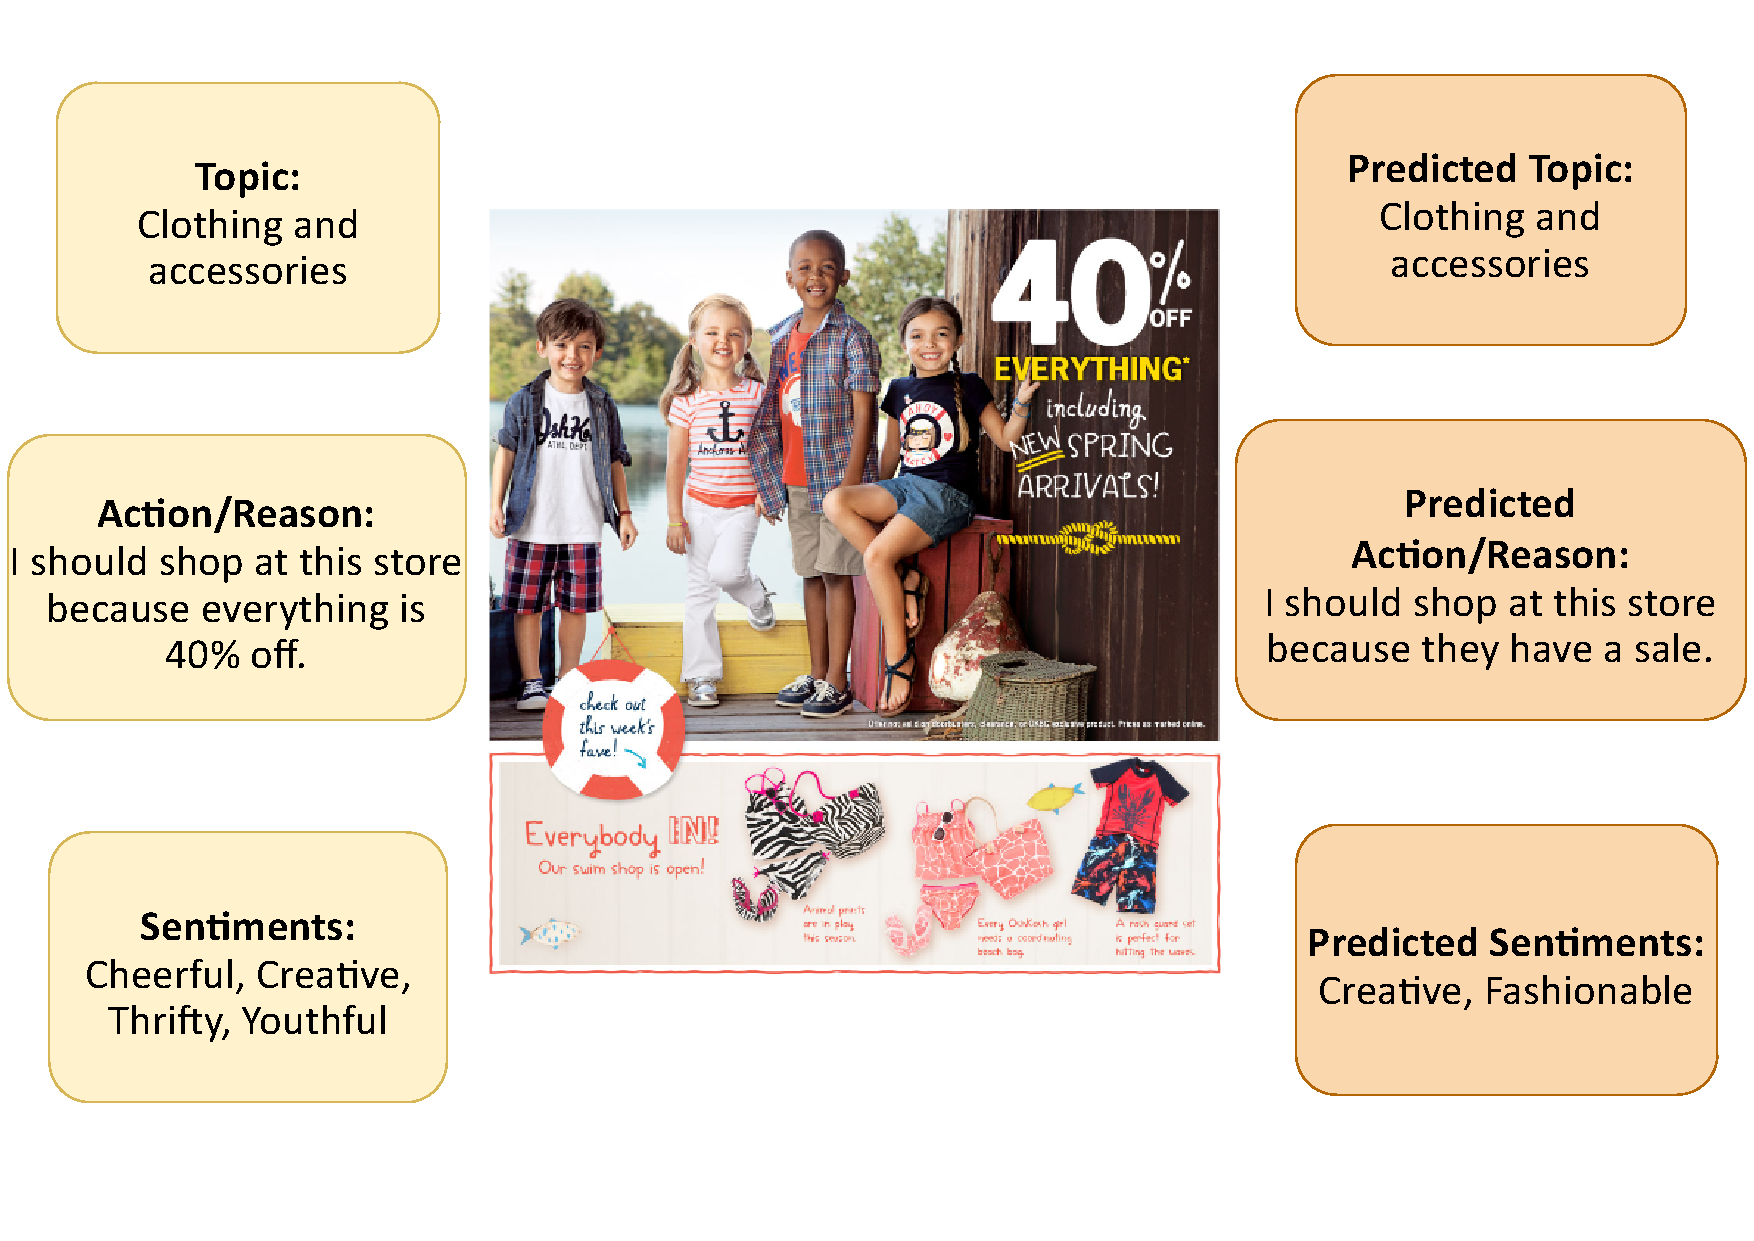
\includegraphics[width=\textwidth,scale=0.68]{images/preds_sup_1.pdf}
         \caption{}
         \label{fig:preds-sup-1}
        %  \vspace{-3pt}
     \end{subfigure}
     \begin{subfigure}[b]{0.49\textwidth}
         \centering
         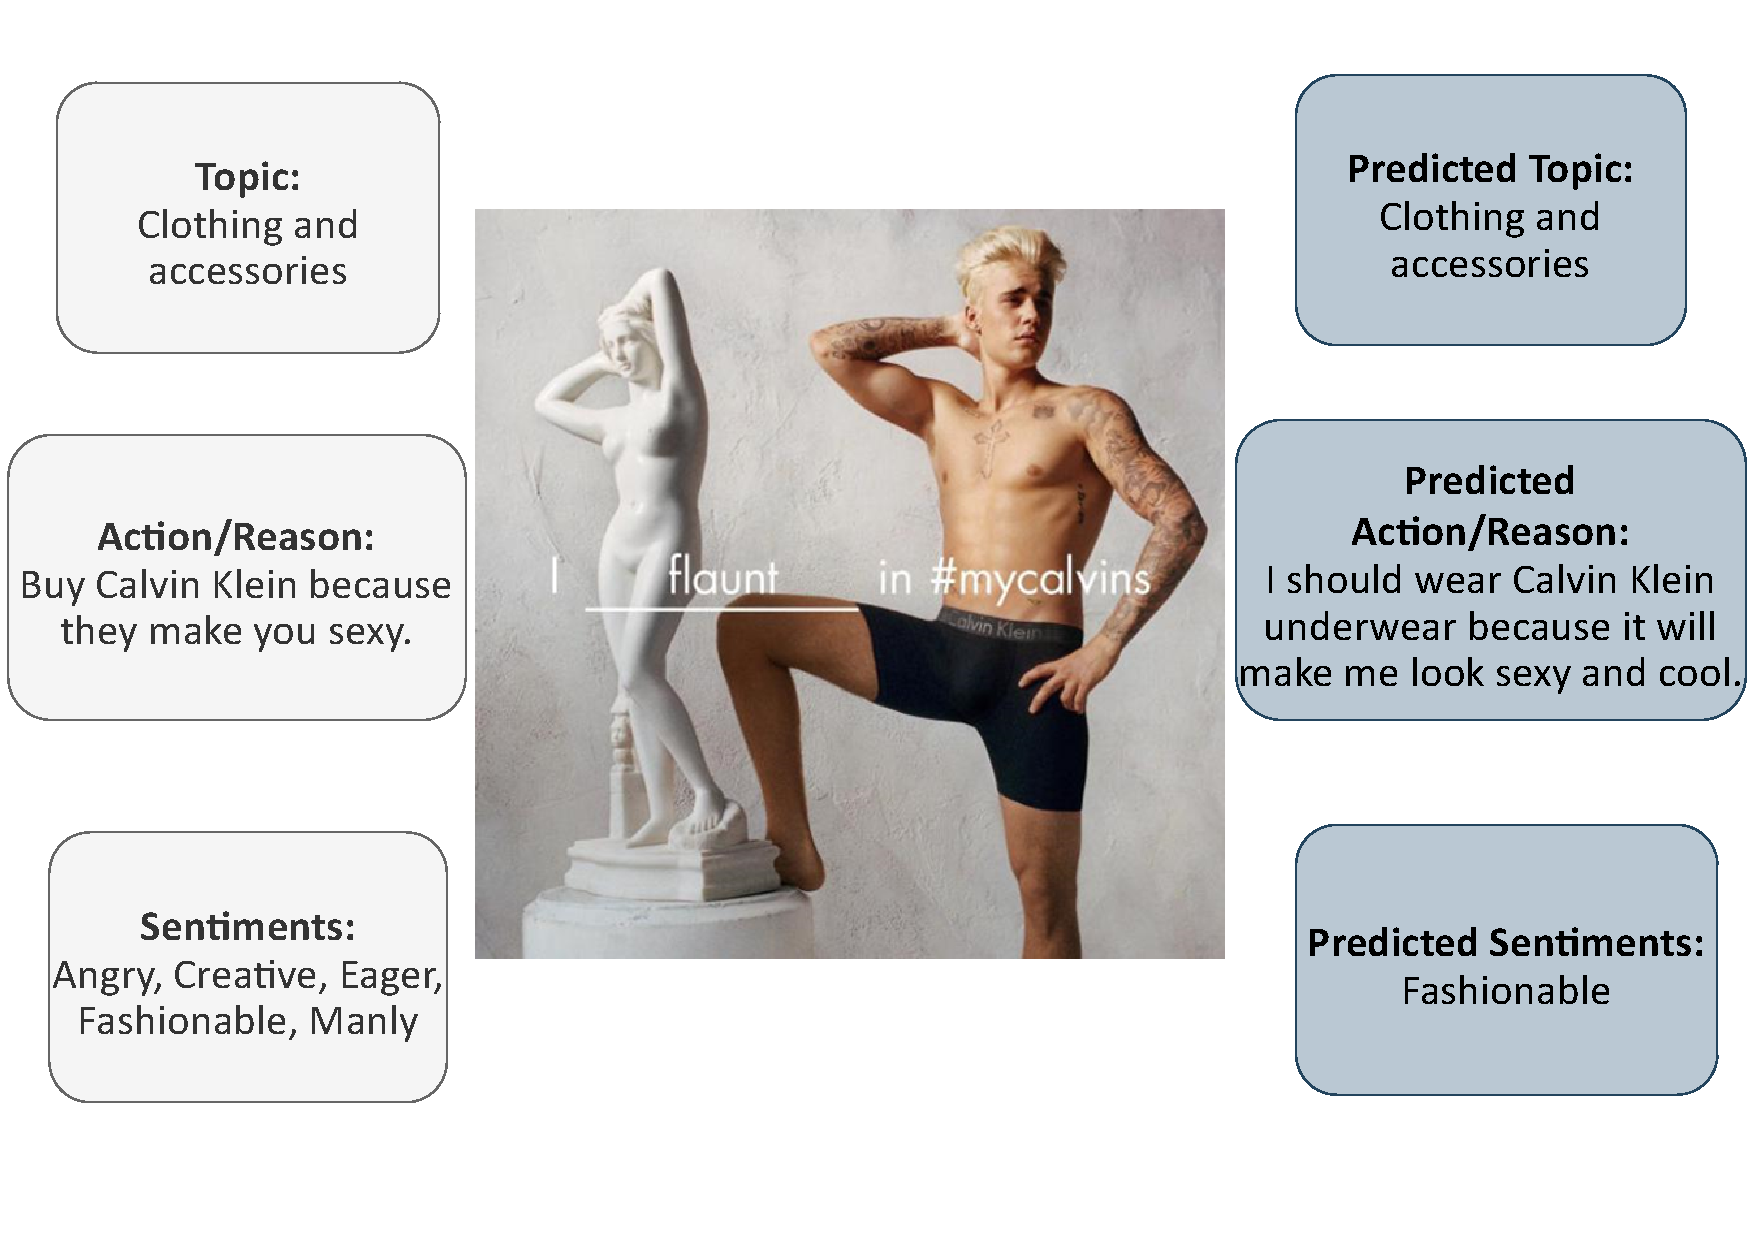
\includegraphics[width=\textwidth,scale=0.68]{images/preds_sup_2.pdf}
         \caption{}
         \label{fig:preds-sup-2}
        %  \vspace{-3pt}
     \end{subfigure}
    %  \begin{subfigure}[b]{0.49\textwidth}
    %      \centering
    %      \includegraphics[width=0.8\textwidth,scale=0.68]{LaTeX/images/preds_sup_5.pdf}
    %      \caption{}
    %      \label{fig:preds-sup-5}
    %      \vspace{-10pt}
    %  \end{subfigure}
     \begin{subfigure}[b]{0.49\textwidth}
         \centering
         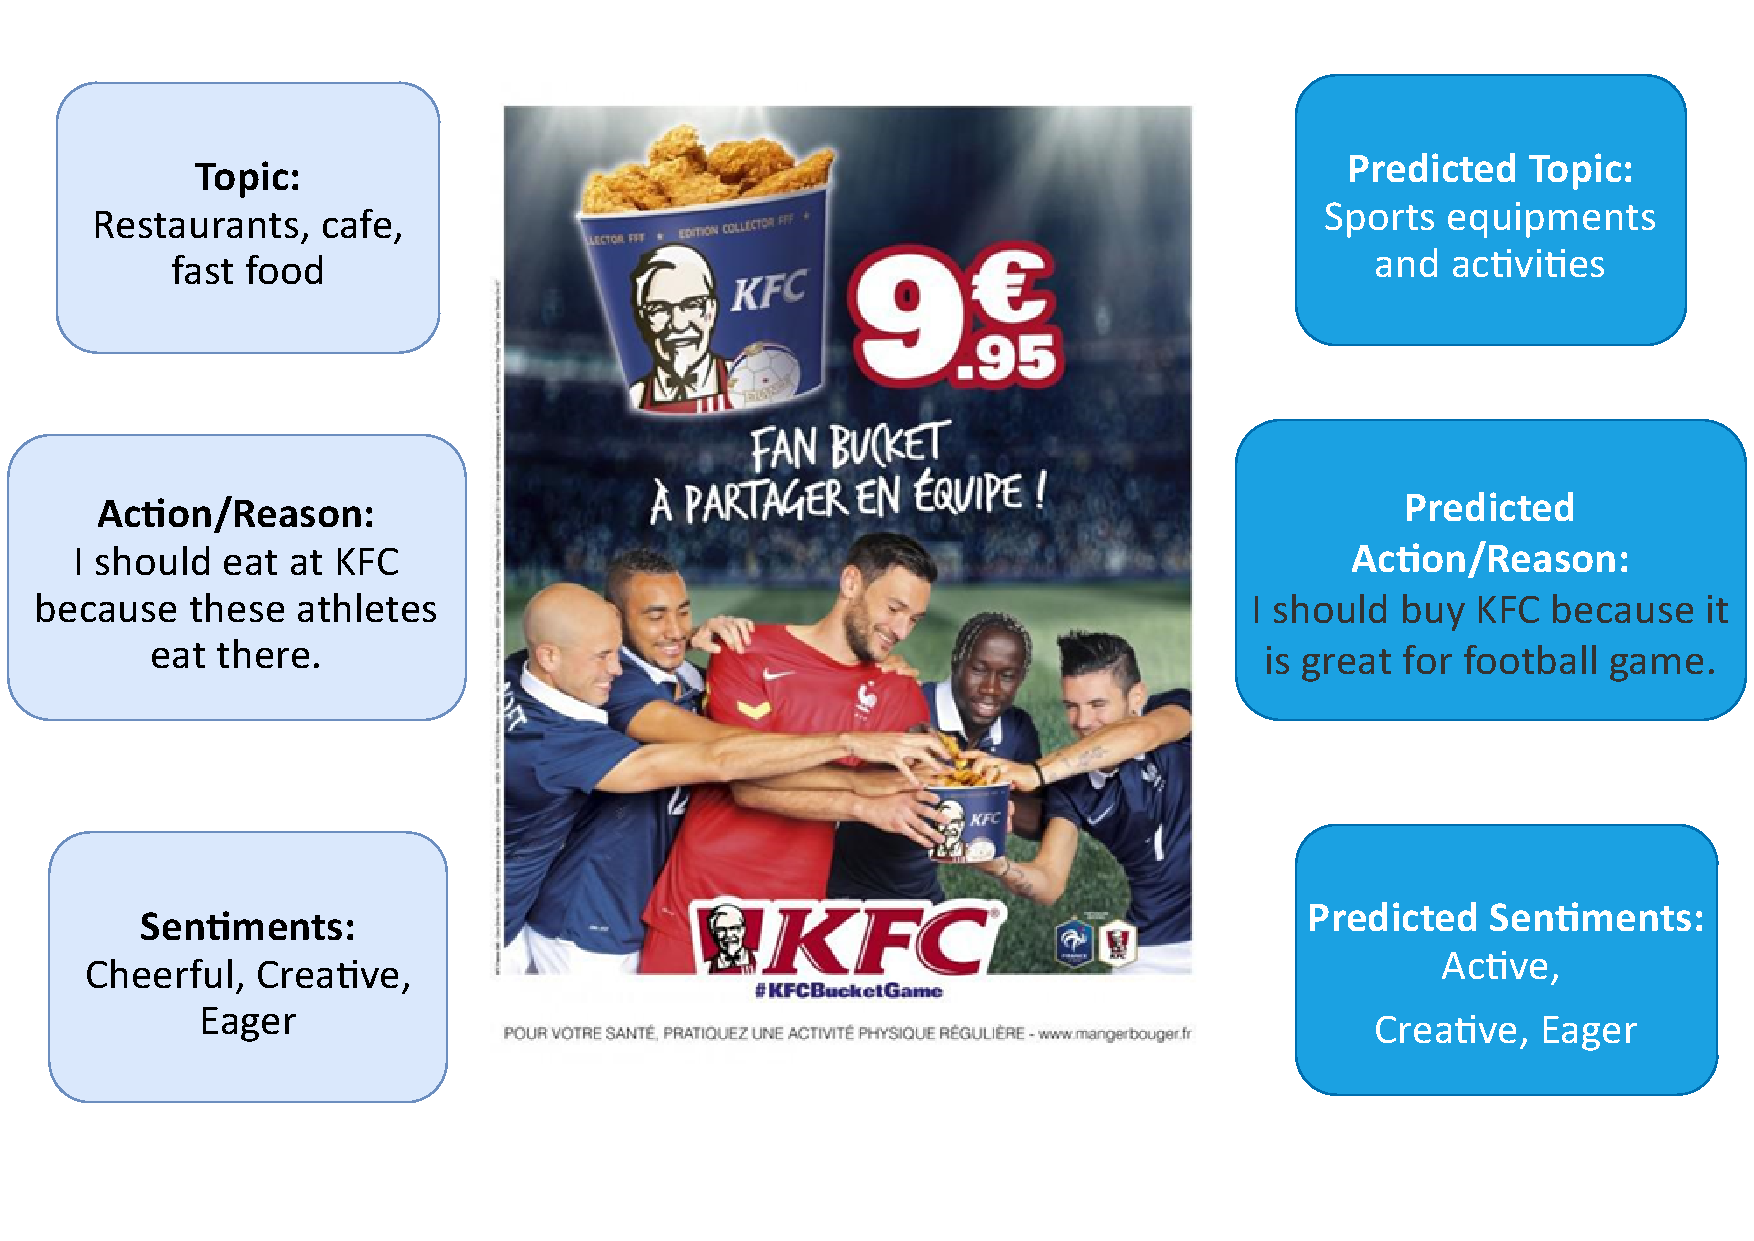
\includegraphics[width=\textwidth,scale=0.68]{images/preds_sup_8.pdf}
         \caption{}
         \label{fig:preds-sup-8}
            % \vspace{-10pt}
     \end{subfigure}
    \caption{Some samples from the Pitts Ads dataset along with the ground truth and predicted action-reason statement, topic and sentiments.}
    \label{fig:preds-sup}
\end{figure}


\subsection{Modelling Persuasion Strategy For Image Advertisements}
The proposed Ads dataset $\mathcal{D}$ annotated with the persuasion strategies comprises of samples where each sample advertisement $a_i$ is annotated with a set of annotation strategies $S_i$ such that $1\le|{S_i}|\le3$. The unique set of the proposed persuasion strategies $\mathcal{P}$ is defined in Table~\ref{tab:persuasive-strategies-list}. Given $a_i$, the task of the modeling is to predict the persuasion strategies present in the input ad. As we observe from Fig.~\ref{fig:persuasion-strategies-headline-image}, advertisements use various rhetoric devices to form their messaging strategy. The strategies thus are in the form of multi-modalities, including images, text and symbolism. To jointly model the modalities, we design an attention fusion multi-modal framework, which fuses multimodal features extracted from the ad, {\it e.g.}, the ad image, text present in the ad extracted through the OCR (Optical Character Recognition), regions of interest (ROIs) extracted using an object detector, and embeddings of captions obtained through an image captioning model (see Fig.~\ref{fig:arch_diag}). The information obtained through these modalities are firstly embedded independently through their modality specific encoders followed by a transformer-based cross-attention module to fuse the extracted features from different modalities. The fused embeddings from the attention module are then used as input for a classifier that predicts a probability score for each strategy $p \in \mathcal{P}$. The overall architecture of the proposed model is illustrated in Fig.\ref{fig:arch_diag}. In the following, we describe each step in the prediction pipeline in detail.






\iffalse
{\small%
\begin{table}[]
\small
      \resizebox{0.8\columnwidth}{!}{%
      \begin{tabular}{ll}
            \toprule
             \textbf{Strategies} & \textbf{Corr}\\ \midrule
              Eager-Concreteness & 0.268 \\\midrule
             Scarcity-Reciprocity & 0.253 \\\midrule
             Eager-Cheerful  & 0.187 \\\midrule
             Amazed-Concreteness & 0.174 \\\midrule
             Eager-Reciprocity & 0.165 \\\bottomrule
        \end{tabular}}
        \caption{\looseness=-1 Top-5 Dice Correlated Persuasion Strategies. In general, we observe that persuasion strategies are not heavily correlated with each other. This means that the marketers are using unique combinations of messaging strategies to market their products.}
        \label{tab:top-5-correlated strategies}
    \end{table}}
\fi

\begin{figure*}[h]
% \vspace*{-11mm}
        \centering
        % \includegraphics[scale=0.28]{images/Model_Architecture.pdf}
        % \includegraphics[scale=0.185]{images/Persuasion Arch Diag - Copy of Model_Architecture-Page-2.drawio.png}
        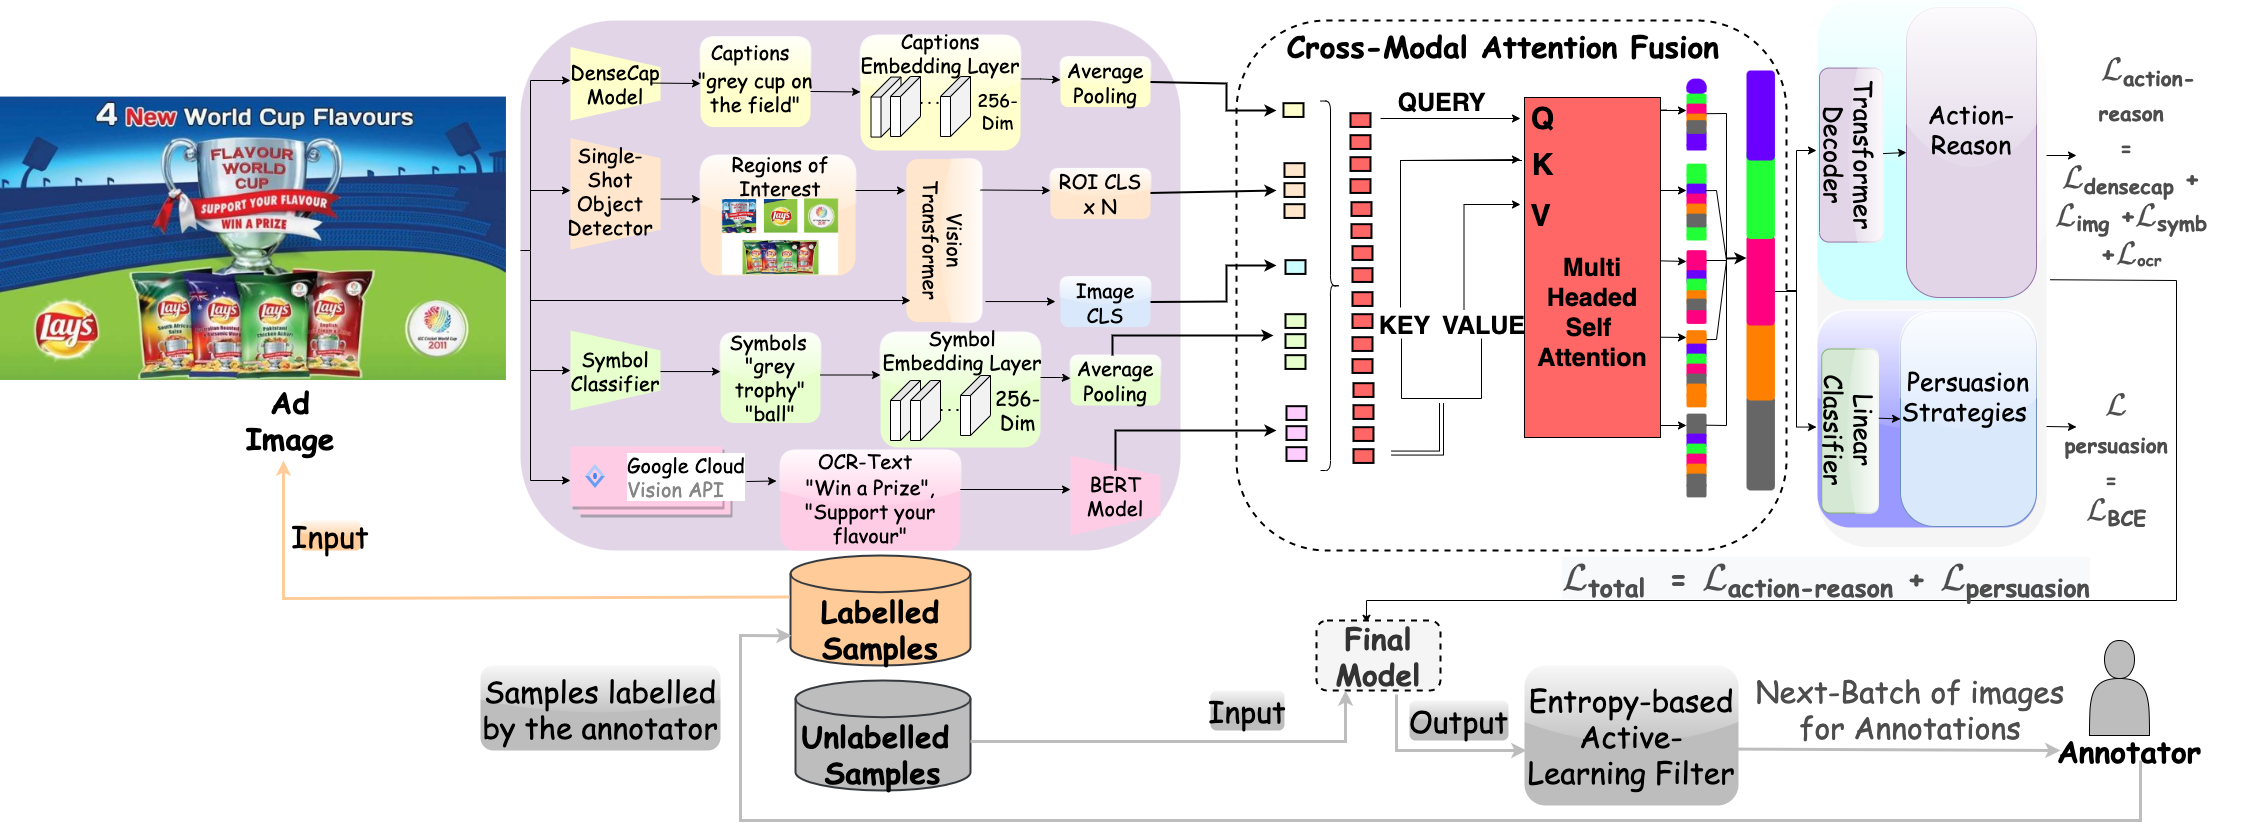
\includegraphics[width=\textwidth]{images/Persuasion-Arch-Diag-Copy-of-Model_Architecture-Page-2.drawio.png}
        % \vspace*{-2mm}
        \caption{\small Architecture of the Persuasion Strategy Prediction model. To capture the different rhetoric devices, we extract features for the image, text, and symbolism modalities and then apply cross-modal attention fusion to leverage the interdependence of the different devices. Further, the model trains over two tasks: persuasion strategies and the reasoning task of action-reason prediction.}
        % \label{fig:persuasion-strategies-headline-image}
% \vspace*{-4mm}
\label{fig:arch_diag}
\end{figure*}




\subsubsection{Feature Extractors} 

In order to capture different rhetoric devices, we extract features from the image, text, and symbolism modalities.

\textbf{Image Feature:} We use the Vision Transformer \cite{dosovitskiy2020image} (ViT) model for extracting image features from the entire input image. The model resizes the input image to size $224 \times 224$ and divides it into patches of size $16 \times 16$. The model used has been pre-trained on the ImageNet 21k dataset. We only use the first output embedding, which is the CLS token embedding, a $768$ dimension tensor, as we only need a representation of the entire image. Then, a fully connected layer is used to reduce the size of the embedding, resulting in a tensor of dimension $256$.




\textbf{Regions of Interest (RoIs) from Detected Objects and Captions:} %The major difference between creative and natural images is the presence of composing elements \cite{zitnick2013bringing,zitnick2014adopting}. 
Ad images contain elements that the creator deliberately chooses to create \textit{intentional impact} and deliver some \textit{message} in addition to the ones that occur \textit{naturally} in the environment. Therefore, it is important to identify the composing elements of an advertisement to understand the creator's intention and the ad's message to the viewer. We detect and extract objects as regions of interest (RoIs) from the advertisement images. We get the RoIs by training the single-shot object detector model \cite{liu2016ssd} on the COCO dataset \cite{lin2014microsoft}. We compare it with the recent YOLOv5 model \cite{redmon2016you}. We also extract caption embeddings to detect the most important activity from the image using a caption generation mode. We compare DenseCap \cite{yang2017dense} and the more recent BLIP \cite{li2022blip} for caption generation.





\textbf{OCR Text:} The text present in an ad presents valuable information about the brand, such as product details, statistics, reasons to buy the product, and creative information in the form of slogans and jingles that the company wants its customers to remember and thus making it helpful in decoding various persuasion strategies. Therefore, we extract the text from the ads and use it as a feature in our model. We use the Google Cloud Vision API for this purpose. All the extracted text is concatenated, and the size is restricted to $100$ words. We pass the text through a BERT model and concatenate the embeddings for those 100 words. Similar to image embeddings, an FC layer is used to convert embeddings to 256 dimensions. The final embedding of the OCR is a tensor of dimension $100 \times 256$. 


\textbf{Symbolism:} While the names of the detected objects convey the names or literal meaning of the objects, creative images often also use objects for their symbolic and figurative meanings. For example, an upward-going arrow represents growth or the north direction or movement towards the upward direction depending on the context; similarly, a person with both hands pointing upward could mean danger (\textit{e.g.}, when a gun is pointed) or joy (\textit{e.g.}, during dancing). In Fig.~\ref{fig:persuasion-strategies-headline-image}, in the creative Microsoft ad, a symbol of a balloon is created by grouping multiple mice together. Therefore, we generate symbol embeddings to capture the symbolism behind the most prominent visual objects present in an ad. We use the symbol classifier by Hussain \textit{et al.} \cite{hussain2017automatic} on ad images to find the distribution of the symbolic elements present and then convert this to a $256$ dimension tensor. %Finally we get a $2 \times 256$ dimension tensor.


\subsubsection{Cross-Modal Attention} 
To capture the inter-dependency of multiple modalities for richer embeddings, we apply a cross-modal attention (CMA) layer~\cite{frank2021vision} to the features extracted in the previous steps. Cross-modal attention is a fusion mechanism where the attention masks from one modality (\textit{e.g.} text) are used to highlight the extracted features in another modality (\textit{e.g.} symbolism). It helps to link and extract common features in two or more modalities since common elements exist across multiple modalities, which complete and reinforce the message conveyed in the ad. For example, the pictures of the silver cup, stadium, and ball, words like ``Australian'', ``Pakistani'', and ``World Cup'' present in the chips ad shown in Fig.~\ref{fig:arch_diag} link the idea of buying \textit{Lays} with supporting one's country's team in the World Cup. Cross attention can also generate effective representations in the case of missing or noisy data or annotations in one or more modalities \cite{frank2021vision}. This is helpful in our case since marketing data often uses implicit associations and relations to convey meaning. 

The input to the cross-modal attention layer is constructed by concatenating the image, RoI, OCR, caption, and symbol embeddings. This results in a $114 \times 256$ dimension input to our attention layer. The cross-modal attention consists of two layers of transformer encoders with a hidden dimension size of $256$. %The rest of the hyper-parameters are similar to the ones given in the original paper \cite{vaswani2017attention}. 
The output of the attention layer gives us the final combined embedding of our input ad. 
Given image embeddings $E_i$, RoI embeddings $E_r$, OCR embeddings $E_o$, caption embeddings $E_c$ and symbol embeddings $E_s$, the output of the cross-attention layer $E_{att}$ is formulated as:
\begin{align}
        \text{Enc}(X) &= \text{CMA}(\left[E_i(X),E_r(X), E_o(X),E_c(X),E_s(X)\right])\,, \nonumber
\end{align}
where $[\ldots,\ldots]$ is the concatenation operation. For the advertisement in Fig.~\ref{fig:arch_diag}, we observed that the caption ``grey cup on the field'' attends to OCR text (containing words like ``win'') and ViT features of the RoI (of ``cup'' and ``field'').

%We propose solving the following tasks for understanding advertisements: action-reason generation, topic classification, and sentiment detection. For solving these, we consider a multi-task learning framework where each task has a task-specific network built upon a common, shared multi-modal encoder. We learn the shared parameters $\thetav_s$ and a set of task-specific parameters $\{\thetav_i\}^{T}_{i=1}$ for $T$ tasks. Our goal is to learn parameters $\thetav_s \cup \{\thetav_i\}^{T}_{i=1}$ that minimize loss across all tasks. Details on different tasks and loss designs are introduced next. In our specific setting, we have $T=3$.


\subsubsection{Persuasion Strategy Predictor} 
This module is a persuasion strategy predictor, which processes the set of feature embedding \text{Enc}(X) obtained through cross-modality fusion. Specifically, \text{Enc}(X) is passed through a self-attention layer as:
\begin{align}
o_{1} = softmax(\text{Enc}(X) \otimes W_{self-attn})^\intercal \otimes \text{Enc}(X)
\end{align}
where \text{Enc}(X) is of the dimension $114\times256$,  $W_{self-attn} \in \mathcal{R}^{256 \times 1}$, $\otimes$ denote tensor multiplication and $o_1$ denotes the output of self attention layer, which is further processed through a linear layer to obtain $o_{|\mathcal{P}|}$ to represent the logits for each persuasion strategy. We apply sigmoid over each output logit such that the $i^{th}$ index of the vector after applying sigmoid denotes $p_i$ - the probability with which $i^{th}$ persuasion strategy is present in the ad image. Our choice of using sigmoid over softmax is motivated by the fact that multiple persuasion strategies can be present simultaneously in an ad image. Consequently, the entire model is trained in an end-to-end manner using binary cross-entropy loss $\mathcal{L}_{s}$ over logit for each strategy:
\begin{align}
        \mathcal{L}_{s} = \left[-y_i \log(p_i) - (1-y_i) \log(1 - p_i) \right]
\end{align}
where, $y_i$ is 1 if $i^{th}$ persuasion strategy is present in the ad and 0 otherwise. It can be observed in Table~\ref{tab:modalities} that our model achieves an accuracy of $59.2\%$, where a correct match is considered if the strategy predicted by the model is present in the set of annotated strategies for a given ad. Further, we perform several ablations where we exclude each modality while retaining all the other modalities. We note that for each modality, excluding the modality results in a noticeable decrease in accuracy, with significant decreases observed when excluding DenseCap ($\sim3.6\%$) and OCR ($\sim4.4\%$). Further, we observe that using DenseCap for obtaining caption embeddings, and SSD for object detection works better than BLIP and YOLOv5, respectively (see Table~\ref{tab:varying_cap_obj}). We also explore using focal loss~\cite{lin2017focal} in place of cross-entropy loss to handle class imbalance but observed that it led to degradation instead of improvements (top-1 acc.\footnote{\textit{Top-1 Accuracy}: It is defined as the fraction of images, where the highest predicted strategy is present in the ground-truth strategies. \textit{Top-3 Accuracy} : It is defined as the fraction of images, where any of the top-3 highest predicted strategies is present in the ground-truth strategies.} of $56.4\%$ \textit{vs} $59.2\%$ using cross-entropy). We also train the model of Hussain \textit{et al.} \cite{hussain2017automatic} for strategy prediction through a similar configuration as ours (along with action-reason generation using an LSTM branch). We find that their top-1 and top-3 accuracy is 52.4\% (vs. 59.2\% ours) and 75.7\% (vs. 84.8\% ours), which is lesser compared to our model.

\begin{table}[t]
% \vspace{-8mm}
    \small
        \centering
        %\begin{adjustbox}{width=\columnwidth,center}
        \resizebox{0.8\columnwidth}{!}{%
       \begin{tabular}{lll}%[tab1,tabularx={XYYYYY}]
             \textbf{\thead{Models}} & \textbf{\thead{Top-1  Acc.}} & \textbf{\thead{Top-3 Acc.}}\\ \midrule
             Our Model & \textbf{59.2} & \textbf{84.8} \\ \midrule
             w/o DenseCap & 55.6 & 80.8 \\ \midrule
             w/o Symbol   & 58.8 & 81.6 \\ \midrule
           w/o DenseCap \& Symbol & 55.2 & 80.8 \\ \midrule
            w/o OCR & 54.8 & 82 \\ \midrule
            w/o Symbol,\\OCR \& DenseCap & 58 & 78.8 \\ \midrule
                %  With Topic & 43.2 & 67.2 \\ \bottomrule
            w/o Action-Reason Task & 56.4 & 80.4\\ \midrule
            Random Guess & 6.25 &  18.75\\\bottomrule
        \end{tabular}}
        \caption{\small Effect of different Modalities and Tasks on the accuracy and performance of the strategy prediction task.}
        % \vspace{-3mm}
        %\end{adjustbox}
        \label{tab:modalities}
    \end{table}

\subsubsection{Multi Task Learning}
One of the key opportunities for our persuasion strategies data labeling and modeling task was the presence of additional labels already given in the base Pitts Ads dataset. In that, authors had given labels about the reasoning task. For the reasoning task, the annotators were asked to provide answers in the form ``I should [Action] because [Reason]." for each ad. In other words, they asked the annotators to describe \textit{what the viewer should do and why}, according to
the ad. Similar to the reasoning task, persuasion strategies provide various cognitive, behavioral, and affective reasons to try to elicit the motivation of the ad viewers towards their products or services. Therefore, we hypothesize that these natural language descriptions of \textit{why the viewers should follow} the ad will be informative in inferring the ad's persuasion strategy.

We formulate obtaining action-reason statement as a sequence generation task where the model learns to generate a sentence $Y^g=(y^g_1, \ldots, y^g_T)$ of length $T$ conditioned on advertisement $X$ by generating the sequence of tokens present in the action-reason statement. To achieve this, we use a transformer decoder module that attends on the features $\text{Enc}(X)$ as shown in Fig.~\ref{fig:arch_diag}. The annotated action-reason statement is used to train the transformer decoder as an auxiliary task to strategy prediction through the standard teacher forcing technique used in Seq2Seq framework. Please refer to the Supplementary for more architectural details about the action-reason generation branch. As shown in Table~\ref{tab:modalities}, generating action-reason as an auxiliary task improves the strategy prediction accuracy by $2.8\%$. We evaluate the performance on action-reason generation on following metrics: BLEU-1, BLEU-2, BLEU-3, BLEU-4, METEOR, ROUGE, CIDER, SPICE and observed a score of 53.6, 42.0, 33.1, 25.7, 26.3, 48.4, 42.8, 8.9 respectively.


% task Ti dataset Di consisting  of ni training  samples,  i.e.,Di={xij,yij}nij=1,  where xij∈Rdi is the jth training instance in Ti and yi ji s its label. We denote byXithe  training  data  matrix  forTi,  i.e.,Xi= (xi1,...,xini)

% \vspace{-1mm}

\begin{table}[!t]
        \small
        \centering
        % \vspace{-8mm}

        %\begin{adjustbox}{width=\columnwidth,center}
        \resizebox{0.8\columnwidth}{!}{%
       \begin{tabular}{llllll}%[tab1,tabularx={XYYYYY}]
                \textbf{\thead{Model Used}} & \textbf{\thead{Top-1 \\Accuracy}} & \textbf{\thead{Top-3 \\Accuracy}} &  \textbf{Recall} \\ \midrule
                 Model with \\DenseCap \& SSD & 59.2 & 84.8 & 74.59\\ \midrule
                 Model with \\BLIP \& YOLOv5 & 58.4 &  83.8 & 71.58 \\ \midrule
        \end{tabular}}
        \caption{\small Comparison of caption and object detection models. We noticed that BLIP while being more recent and trained on a larger dataset, generates more informatory captions for background objects which DenseCap successfully ignores.}
        % \vspace{-3mm}
        %\end{adjustbox}
        \label{tab:varying_cap_obj}
    \end{table}
        \begin{figure}[h]
        \centering
        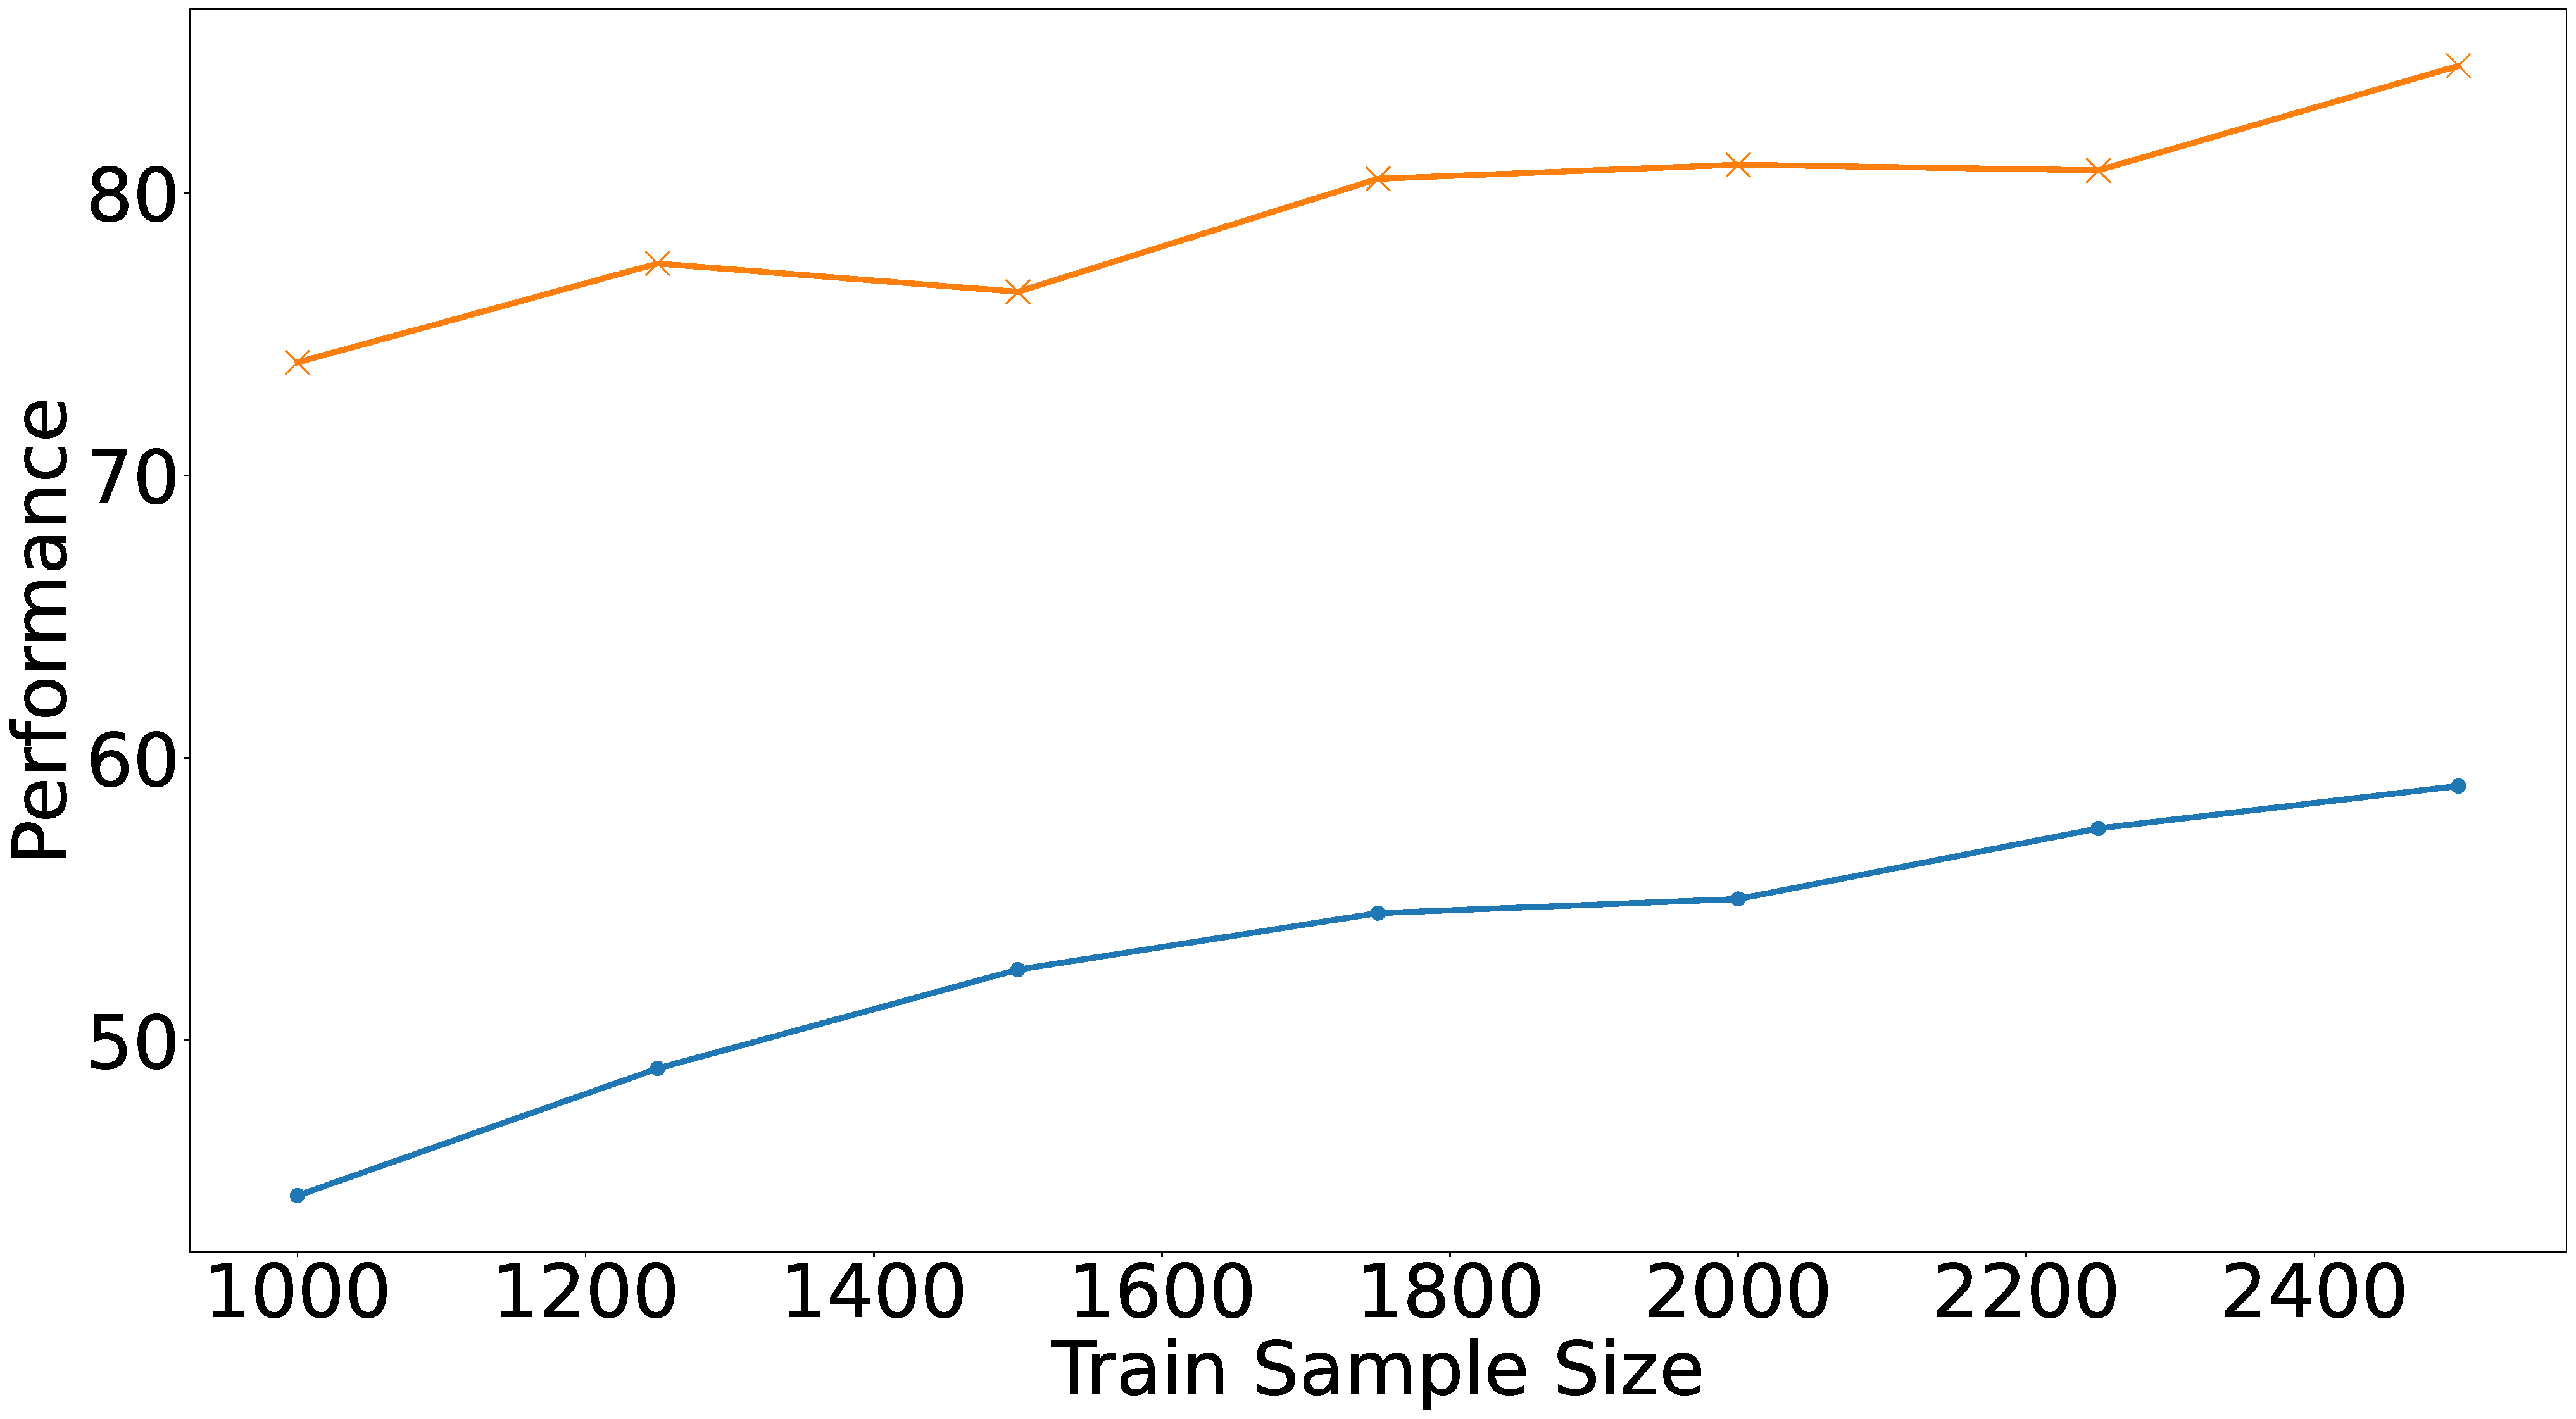
\includegraphics[scale=0.12]{images/active_learning.pdf}
        \caption{\small Incremental effect of introducing new data through active learning; Results for prediction of persuasion strategies on the test set}
        % \vspace{-4mm}
        \label{fig:AL_batch_test}
    \end{figure}


\begin{table}[]
    \small
        \centering
        %\begin{adjustbox}{width=\columnwidth,center}
        \resizebox{\textwidth}{!}{%
       \begin{tabular}{llllll}%[tab1,tabularx={XYYYYY}]
             & \textbf{\thead{\#ads with \\1 strategy}} & \textbf{\thead{\#ads with \\2 strategies}} & \textbf{\thead{\#ads with \\3 strategies}} & \textbf{\thead{Avg.\\strategies}} & \textbf{\thead{Std.\\Dev.}}\\ \midrule
             Train-Set & 1440 & 905 & 155 & 1.486 & 0.612 \\\midrule
             Val-Set & 132 & 98 & 20 & 1.552  & 0.639 \\\midrule
             Test-Set & 147 & 93 & 10 & 1.452 &0.574\\\midrule\midrule
             Total & 1719 & 1096 & 185 & 1.49 & 0.592 \\\bottomrule
        \end{tabular}}
        \caption{\small Distribution of test, train, validation, and the total dataset}
        \label{table:strategy-train-test-val-stats}
        % \vspace*{-3mm}
        %\end{adjustbox}
    \end{table}



\subsubsection{Active Learning}
We use an active learning method to ease the large-scale label dependence when constructing the dataset. As in every active learning setting, our goal is to develop a learner that selects samples from unlabeled sets to be annotated by an oracle. Similar to traditional active learners \cite{gilad2005query,lewis1994heterogeneous}, we use uncertainty sampling to perform the sample selection. In doing so, such function learns to score the unlabeled samples based on the expected performance gain they are likely to produce and used to update the current version of the localization model being trained. To evaluate each learner, we measure the performance improvements, assessed on a labeled test set at different training dataset sizes.


At every learning step $t$, a set of labeled samples $L_t$ is first used to train a model
$f_t$. Then, from an unlabeled pool $U_t=D-L_t$, an image instance $a$ is chosen by a selection function $g$. Afterwards, an oracle provides temporal ground-truth for the selected instance, and the labeled set $L_t$ is augmented with this new annotation. This process repeats until the desired performance is reached or the set $U_t$ is empty.

In our implementation, we instantiate the active learning selection function as the entropy of the probability distribution predicted by the model over the set of persuasion strategies for a given ad image instance $a$. Formally, $g = -\sum_{i=1}^{|\mathcal{P}|}p^{n}_{i}*\log(p^{n}_i)$, where $p^{n}_i$ denotes the normalized probability with which $i^{th}$ persuasion strategy is present in $a$ as per the model prediction. The normalized probability $p^{n}_{i}$ is estimated as $p_i/\sum_{j=1}^{|\mathcal{P}|}p_j$. Intuitively, ad samples with high entropy selection values indicate that the model trained on limited data has a higher degree of confusion while predicting the persuasion strategy since it is not decisively confident about predicting few strategies. Hence, we rank the unlabeled ad images in the decreasing order of difficulty according to the corresponding values of the entropy selection function and select the top-k ads in the subsequent batch for annotation followed by training. As shown in Fig.~\ref{fig:AL_batch_test}, we set k to be 250 and analyze the effect of incrementally introducing new samples selected through active learning. It can be seen that both top-1 and top-3 accuracy increases with the addition of new training data. We stop at the point when 2500 training samples are used since the model performs reasonably well with a top-1 and top-3 strategy prediction accuracy of 59.2\% and 84.8\% (see Fig.~\ref{fig:AL_batch_test}). 



%%%%%%%%%%%%%%%%%%%%%%%%%%%%%%%%%%%%%%%%%%%%%%%%%%%%%%%%%%%%%%%%%%%%
%%%%%%%%%%%%%%%%%%%%%%%%%%%%%%%%%%%%%%%%%%%%%%%%%%%%%%%%%%%%%%%%%%%%



\subsection{Modelling Persuasion Strategy For Video Advertisements}
Large Language Models (LLMs) have been demonstrated to perform well for downstream classification tasks in the text domain. This powerful ability has been widely verified on natural language tasks, including text classification, semantic parsing, mathematical reasoning, \textit{etc}. Inspired by these advances of LLMs, we aim to explore whether they could tackle reasoning tasks on multimodal data (\textit{i.e.} videos). Therefore, we propose a storytelling framework, which leverages the power of LLMs to verbalize videos in terms of a text-based story and then performs downstream video understanding tasks on the generated story instead of the original video. Our pipeline can be used to verbalize videos and understand videos to perform complex downstream tasks such as emotion, topic, and persuasion strategy detection. 


We show the performance of our framework on fifteen distinct tasks across five datasets. Firstly, we employ a video story dataset to evaluate the story generation task. Secondly, we utilize a video advertisements dataset to assess topic and emotion classification, as well as action and reason generation. Then, the persuasion strategy dataset to evaluate the task of understanding persuasion strategies within stories, and finally, HVU and LVU for concept, user engagement, and attribute prediction. These diverse datasets allow us to evaluate the performance and capabilities of our framework thoroughly.


\textbf{1.~The Video story dataset} \cite{Li_2020} contains 105 videos, from four types of common and complex events (\textit{i.e.} birthday, camping, Christmas, and wedding) and corresponding stories written by annotators. It has longer videos (average length 12.4 mins) and longer descriptions (162.6 words on average).
Moreover, the sentences in the dataset are more sparsely distributed across the video (55.77 sec per sentence).
\textit{Metrics}: Following \cite{Li_2020}, we use several NLP metrics, \textit{viz.}, BLEU-N, ROUGE-L, METEOR and CIDEr to measure the similarity between the story generated by the model and ground truth.


\textbf{2.~The Image and Video Advertisements} \cite{hussain2017automatic} contains 3,477 video advertisements and the corresponding annotations for emotion and topic tags and action-reason statements for each video. There are a total of 38 topics and 30 unique emotion tags per video. Further, we have 5 action-reason statements for each video for the action-reason generation task. For our experiment, we use 1785 videos, due to other videos being unavailable/privated from Youtube.

\textit{Metrics}: Following \cite{hussain2017automatic}, for the topic and emotion classification task, we evaluate our pipeline using top-1 accuracy as the evaluation metric. Further, since \cite{hussain2017automatic} did not use any fixed set of vocabulary for annotations, rather they relied on annotator-provided labels, the labels are often very close (like cheerful, excited, and happy). Therefore, based on nearness in Plutchik's \cite{PLUTCHIK19803} wheel of emotions, we club nearby emotions and use these seven main categories: joy, trust, fear, anger, disgust, anticipation, and unclear. For the action-reason task, following \cite{hussain2017automatic}, we evaluate our accuracy on the action and reason retrieval tasks where 29 random options along with 1 ground truth are provided to the model to find which one is the ground truth. Further, we also generate action and reason statements and evaluate the generation's faithfulness with the ground truth using metrics like ROUGE, BLEU, CIDEr, and METEOR.


\textbf{3.~Persuasion strategy dataset}: This is the dataset we contribute for understanding persuasion strategies.

\textit{Metrics}: We evaluate the performance using top-1 accuracy metric. Videos have a varied number of strategies, therefore, we consider a response to be correct if the predicted strategy is present among the list of ground-truth strategies.


\textbf{4.~Long-Form Video Understanding (LVU)}: We \textit{et al.} \cite{wu2021towards} released a benchmark comprising of 9 diverse tasks for long video understanding and consisting of over 1000 hours of video. The various tasks consist of content understanding (`relationship', `speaking style', `scene/place'), user engagement prediction (`YouTube like ratio', `YouTube popularity'), and movie metadata prediction (`director', `genre', `writer', `movie release year'). We \textit{et al.} \cite{wu2021towards} use top-1 classification accuracy for content understanding and metadata prediction tasks and MSE for user engagement prediction tasks.


\textbf{5.~Holistic Video Understanding (HVU)}: 
HVU \cite{diba2020large} is the largest long video understanding dataset consisting of 476k, 31k, and 65k samples in train, val, and test sets, respectively. A comprehensive spectrum includes the identification of various semantic elements within videos, consisting of classifications of scenes, objects, actions, events, attributes, and concepts. To measure performance on HVU tasks, similar to the original paper, we use the mean average precision (mAP) metric on the validation set.




\begin{figure*}[!t]
  \includegraphics[width=0.99\textwidth]{images/verbalizing-marketing-graphics.pdf}
  \caption{The overview of our framework to generate a story from a video and perform downstream video-understanding tasks. First, we sample keyframes from the video which are verbalized using BLIP-2. We also extract OCR from all the frames. Next, using the channel name and ID, we query Wikidata to get company and product information. Next, we obtain automatically generated captions from Youtube videos using the Youtube API. All of these are concatenated as a single prompt and given as input to an LLM and ask it to generate the story of the advertisement. Using the generated story, we then perform the downstream tasks of emotion and topic classification and persuasion strategy identification. This video can be watched at \url{https://youtu.be/ZBLkTALi1CI}.
  %\url{https://github.com/Aanisha/persuasion-advertisements/blob/main/videos/ZBLkTALi1CI.mp4}.
  }
  \label{fig:story-generation-pipeline}
\end{figure*}



Next, we explain our pipeline to solve these tasks.

\subsubsection{Video Verbalization} 
To obtain a verbal representation of a video, we employ a series of modules that extract unimodal information from the multimodal video. This information is then used to prompt a generative language model (such as GPT-3.5 \cite{brown2020language} and Flan-t5 \cite{chung2022scaling}) to generate a coherent narrative from the video. The overall pipeline is depicted in Fig.~\ref{fig:story-generation-pipeline}. In the following, we delve into each component of the framework in details.

\noindent \textbf{1. Video Metadata:} Understanding the context of a story is crucial, and we achieve this by gathering information about the communicator (brand). We leverage the publicly available video title and channel name from the web. Additionally, we utilize Wikidata \cite{10.1145/2629489}, a collaborative knowledge base that provides comprehensive data for Wikipedia, to obtain further details such as the company name, product line, and description. This information helps us comprehend the story elements and establish connections with the brand's business context. For non-advertisement videos, we skip this step and retrieve only the video title.

\noindent \textbf{2. Text Representation of Video Frames:} We extract two types of textual information from video frames. Firstly, we capture the literal text present on the frames. Secondly, we analyze the scene depicted in each frame to gain a deeper understanding. In the upcoming sections, we will elaborate on both of these aspects.


\begin{table*}[!h]\centering
% \scriptsize
\begin{adjustbox}{max width = 0.9\textwidth}
\begin{tabular}{llccccccc}\toprule[1.5pt]
\textbf{Method} &\textbf{Frame Extraction} &\textbf{METEOR} & \textbf{CIDEr} &\textbf{Rougle-l} &\textbf{BLEU-1}&\textbf{BLEU-2}&\textbf{BLEU-3}&\textbf{BLEU-4}\\\toprule[0.5pt]
GPT-3.5 & Uniform Sampling & 24.8 & 102.4 & 24.3 & 63.8 & 56.4 & 47.2 & 38.6 \\
GPT-3.5 & Pyscenedetect & 24.17 & 67.8 & 21.17 & 54.59 & 49.05 & 41.54 & 33.88 \\\bottomrule[1.5pt]
\end{tabular}
\end{adjustbox}
\caption{Comparison of Pyscenedetect \cite{breakthrough-pyscenedetect} with uniform sampling of choosing video frames. Based on downstream performance, we can see that uniform sampling works better than Pyscenedetect  \label{tab:ablation-sampling}}
\end{table*}

\textit{a. Visual and Scenic Elements in Frames:} For videos with a duration shorter than 120 seconds, we employ an optical flow-based heuristic using the GMFlow model \cite{xu2022gmflow} to extract keyframes. In shorter advertisement videos, scene changes often indicate transitions in the story, resulting in keyframes with higher optical flow values. The GMFlow model effectively captures these story transitions. We select frames with an optical flow greater than 50 and prioritize frames with maximum pixel velocity. However, for longer videos, this approach yields a large number of frames that are difficult to accommodate within a limited context. To address this, we sample frames at a uniform rate based on the native frames-per-second (fps) of the video (see Table~\ref{tab:ablation-sampling} for a comparison between uniform sampling and Pyscenedetect). Additionally, we discard frames that are completely dark or white, as they may have high optical flow but lack informative content.

Using either of these methods, we obtain a set of frames that represent the events in the video. These frames are then processed by a pretrained BLIP-2 model \cite{li2023blip2}. The BLIP model facilitates scene understanding and verbalizes the scene by capturing its most salient aspects. We utilize two different prompts to extract salient information from the frames. The first prompt, ``\textit{Caption this image}", is used to generate a caption that describes what is happening in the image, providing an understanding of the scene. The second prompt, ``\textit{Can you tell the objects that are present in the image?}", helps identify and gather information about the objects depicted in each frame.


\begin{figure*}[!t]
    \centering
    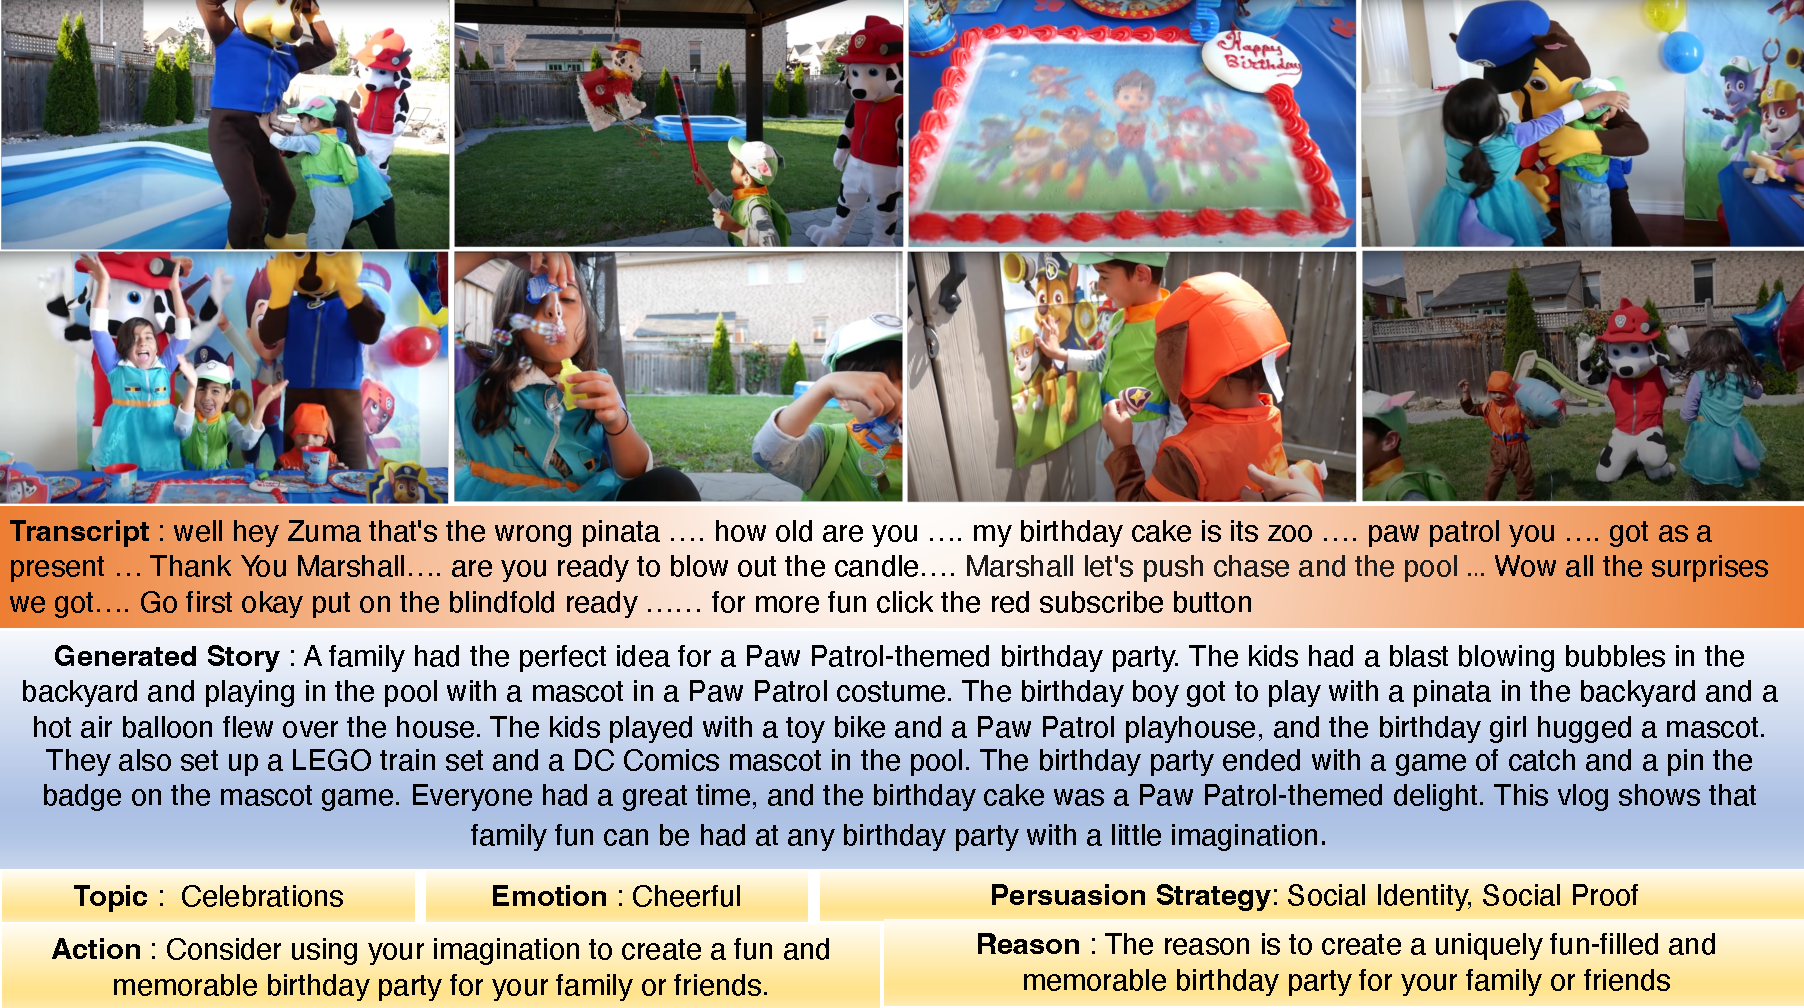
\includegraphics[width=0.8\textwidth]{images/example-stories.pdf}
    \caption{An example of a story generated by the proposed pipeline along with the predicted outputs of the video-understanding tasks on the generated story. The generated story captures information across scenes, characters, event sequences, dialogues, emotions, and the environment. This helps the downstream models to get adequate information about the video to reason about it correctly. The original video can be watched at \url{https://youtu.be/_amwPjAcoC8}.}
    \label{fig:example-story}
\end{figure*}


\textit{b. Textual elements in frames:} We also extract the textual information present in the frames, as text often reinforces the message present in a scene and can also inform viewers on what to expect next \cite{9578608}. 
For the OCR module, we sample every 10th frame extracted at the native frames-per-second of the video, and these frames are sent to PP-OCR \cite{10.1145/2629489}. We filter the OCR text and use only the unique words for further processing.

\noindent \textbf{3. Text Representation of Audio:} The next modality we utilize from the video is the audio content extracted from it. We employ an Automatic Speech Recognition (ASR) module to extract transcripts from the audio. Since the datasets we worked with involved YouTube videos, we utilized the YouTube API to extract the closed caption transcripts associated with those videos.

\noindent \textbf{4. Prompting:} We employ the aforementioned modules to extract textual representations of various modalities present in a video. This ensures that we capture the audio, visual, text, and outside knowledge aspects of the video. Once the raw text is collected and processed, we utilize it to prompt a generative language model in order to generate a coherent story that represents the video. To optimize the prompting process and enable the generation of more detailed stories, we remove similar frame captions and optical character recognition (OCR) outputs, thereby reducing the overall prompt size. %\cy{Do we simply concantenate all the text as the prompt? in what order?}

The prompt template is given in Section~\ref{sec:prompt-format}. Through experimentation, we discovered that using concise, succinct instructions and appending the text input signals (such as frame captions, OCR, and automatic speech recognition) at the end significantly enhances the quality of video story generation. For shorter videos (up to 120 seconds), we utilize all available information to prompt the LLM for story generation. However, for longer videos, we limit the prompts to closed captions and sampled frame captions. The entire prompting pipeline is zero-shot and relies on pre-trained LLMs. In our story generation experiments, we employ GPT-3.5 \cite{brown2020language}, Flan-t5 \cite{chung2022scaling}, and Vicuna \cite{vicuna2023}. A temperature of 0.75 is used for LLM generation. The average length of the generated stories is 231.67 words. Subsequently, these generated stories are utilized for performing video understanding tasks.



\subsubsection{Prompt format} 
\label{sec:prompt-format}
 For verbalization, a template prompt format has been used, including all the data components as objects, captions, asr, ocr, meta-data. 

\textit{``Please write a coherent story based on the following video advertisement. Use only the information provided and make sure the story feels like a continuous narrative and at the end include one sentence about what product the advertisement was about. Do not include any details not mentioned in the prompt.Use the elements given below to create a coherent narrative,but don't use them as it is.The advertisement for the company \{company\_name\} The video is titled \{title\}, with captions that include \{caption\}, voice-over : \{transcripts\}, and object recognition descriptions : \{ocr\}. The following objects are present in the advertisement and should be used to help create the story: \{objects\} Please exclude any empty or stop words from the final text.''}

For downstream tasks, a template prompt format with an instruction about the specific task,the previous generated verbalization and vocabulary for the downstream task is prompted to the LLM. Here is the example for the topic detection task, for other tasks context and vocab were changed accordingly.

\textit{``Given \{topics\} identify the most relevant topic from the dictionary keys from topic\_vocab related to the story of the video advertisement given below.Consider the definitions given with topics in the topic\_vocab dictionary, to identify which topic is most relevant, don't add any extra topics that are not given in dictionary keys and answer with just the most relevant topic. Story : \{verbalization\}''}


\begin{table*}[!h]\centering
% \scriptsize
\begin{adjustbox}{width=\textwidth}
\begin{tabular}{llccccccc}\toprule[1.5pt]
\multirow{2}{*}{\textbf{Training}} & \multirow{2}{*}{\textbf{Model}} &\textbf{Topic} &\multicolumn{2}{c}{\textbf{Emotion}} & \textbf{Persuasion} &\textbf{Action} &\textbf{Reason}\\\cmidrule{4-5}
& & & \textbf{All labels} & \textbf{Clubbed} \\ \midrule[0.5pt]
Random & Random & 2.63 & 3.37 & 14.3 & 8.37 & 3.34 & 3.34 \\\hline
Finetuned & VideoMAE \cite{tong2022videomae} & 24.72 & 29.72 & \valgood{85.55}  & 11.17  & - & - \\
& Hussain \textit{et al.} \cite{hussain2017automatic} & 35.1 & 32.8 & -  & - & - & 48.45 \\
\ & Intern-Video \cite{wang2022internvideo} & 57.47 & \valbest{36.08} & \valbest{86.59} & 5.47 & 6.8 & 7.1 \\\hline
Zero-shot & VideoChat \cite{li2023videochat} & 9.07 & 3.09 & 5.1 &  10.28 & - & - \\

\hline
\textbf{Our Framework} & \makecell{GPT-3.5 Generated Story +\\GPT-3.5 Classifier} & 51.6 & 11.68 & 79.69 &  35.02 &  66.27 & 59.59 \\
Zero-shot & \makecell{GPT-3.5 Generated Story +\\Flan-t5-xxl Classifier} & \valgood{60.5} & 10.8 & 79.10 &  \valgood{33.41} &  \valbest{79.22} & \valbest{81.72} \\
& \makecell{GPT-3.5 Generated Story +\\Vicuna Classifier} & 22.92 & 10.8 & 67.35 & 29.6 & 21.39 & 20.89 \\
& \makecell{Vicuna Generated Story +\\GPT-3.5 Classifier} & 46.7 & 5.9 & 80.33 & 27.54 & 61.88 & 55.44 \\
& \makecell{Vicuna Generated Story +\\Flan-t5-xxl Classifier} & 57.38 & 9.8 & 76.60 & 30.11 & \valgood{77.38} & \valgood{80.66}  \\
& \makecell{Vicuna Generated Story +\\Vicuna Classifier} & 11.75 & 10.5 & 68.13 & 26.59 & 20.72 & 21.00  \\\cmidrule{2-8}
Finetuned & \makecell{Generated Story +\\Roberta Classifier} & \valbest{71.3} & \valgood{33.02} & 84.20 & \valbest{64.67} & 42.96\footnotemark[1] & 39.09\footnotemark[1] \\
% & BLIP-2 Captions + Flant-t5-xl & 32.2 & 7.4 & 43.11 &  32.1 & 52.98 & 76.26 \\
% & BLIP-2 Captions + GPT-3.5 & 32.7 & 7.9 & 76.3 & 30.1 & 49.91 & 58.71 \\

\bottomrule[1.5pt]
\end{tabular}
\end{adjustbox}
\caption{Comparison of all the models across topic, emotion, and persuasion strategy detection tasks. We see that our framework, despite being zero-shot, outperforms finetuned video-based models on the topic classification, persuasion strategy detection and action and reason classification tasks and comes close on the emotion classification task. Further, the Roberta classifier trained on generated stories outperforms both finetuned and zero-shot models on most tasks. Best models are denoted in \valbest{green} and runner-ups in \valgood{blue}.\label{tab:topic-sentiment}}
\end{table*}



\begin{table*}[!th]
  \centering
  % \begin{tabular}{cccccccccc}
  \begin{adjustbox}{width=\textwidth}
  \begin{tabular}{cccccccccc}
    \toprule
    & Method & Model Type & METEOR & CIDEr & ROUGE-L & BLEU-1 & BLEU-2 & BLEU-3 & BLEU-4 \\
    \midrule
    
    Random & Random  & Retrieval  & 13.1 & 30.2 & 21.4 & 43.1 & 23.1 & 10.0 & 4.8 \\\hline
    %\textbf{Finetuned} & CCA \cite{5540112} & Retrieval & 16.5 & 71.8 & 26.7 & 60.1 & 34.7 & 11.8 & 10.1 \\
    %& Uniform \cite{Li_2020}  & Retrieval & 18.3 &  89.9 & 28.0 & 65.7 & 40.6 & 23.2 & 13.2 \\
    %& SeqDPP \cite{NIPS2014_0eec27c4}  & Retrieval & 18.3 & 91.6 & 28.3 & 66.3 & 41.0 & 23.6 & 13.1 \\
    %& Submodular \cite{7298928} & Retrieval & 18.4 & 92.0 & 28.1 & 66.4 & 41.0 & 23.8 & 13.3 \\
    %& vsLSTM \cite{zhang2016video} & Retrieval & 18.2 & 92.4 & 28.2 & 66.6 & 41.5 & 24.1 & 13.6 \\
    %\textbf{Finetuned} & Narrator IoU \cite{Li_2020} & Retrieval & 18.6 & 93.7 & 28.2 & 67.9 & 42.1 & 24.7 & 14.1 \\
    %& Narrator w/o x \cite{Li_2020} & Retrieval & 18.5 & 93.4 & 28.3 & 67.3 & 41.6 & 24.5 & 14.2 \\
    %\textbf{Finetuned} & Narrator w/o f\_(l) \cite{Li_2020} & Retrieval & 19.0 & 96.1 & 29.1 & 68.6 & 42.9 & 25.2 & 14.5 \\
    \textbf{Finetuned} & Narrator \cite{Li_2020} & Retrieval & 19.6 & 98.4 & 29.5 & 69.1 & 43.0 & 25.3 & 15.0 \\
    %& \citet{xu2015show} & Retrieval & 17.7 & 79.5 & 28.0 & 61.7 & 36.4 & 20.2 & 11.5 \\
    %& m-RNN \cite{10.5555/2886521.2886647} & Retrieval & 18.0 & 81.3 & 28.5 & 61.9 & 37.0 & 21.1 & 11.8 \\
    & EMB \cite{Li_2020} & Retrieval & 19.1 & 88.8 & 28.9 & 64.5 & 39.3 & 22.7 & 13.4 \\
    & BRNN \cite{Li_2020} & Retrieval & 18.1 & 81.0 & 28.3 & 61.4 & 36.6 & 20.3 & 11.3 \\
    & ResBRNN \cite{Li_2020} & Retrieval & 19.6 & 94.3 & 29.7 & 66.0 & 41.7 & 24.3 & 14.7 \\
    & \makecell{Pseudo-GT+\\ResBRNN-kNN \cite{Li_2020}} & Retrieval & 20.1 & 103.6 & 29.9 & 69.1 & 43.5 & 26.1 & 15.6 \\
    & GVMF \cite{https://doi.org/10.1049/ell2.12525} & Retrieval & 20.7 & \valgood{107.7} & \valbest{30.8} & \valbest{70.5} & 44.3 & 26.9 & 15.9 \\    \hline
    %& S2VT \cite{venugopalan2015sequence}  & Generative & 14.3 & 64.0 & 28.6 & 63.3 & 40.6 & 24.6 & 15.4 \\
    %& H-RNN \cite{yu2017hierarchicallyattentive} & Generative & 15.5 & 64.6 & \valgood{28.8} & 61.6 & 41.4 & 26.3 & 16.1 \\
    \textbf{Zero-shot} & VideoChat \cite{li2023videochat} & Generative & 15.49 & 42.9 & 17.88 & 50.00 & 43.30 & 34.76 & 27.21 \\\hline
    
   \textbf{\makecell{Zero-shot}} & GPT-3.5 & Generative & \valbest{24.8} & 102.4 & 24.3 & \valgood{63.8} & \valgood{56.4} & \valgood{47.2} & \valbest{38.6} \\
    Our Framework & Vicuna & Generative & 17.4 & 73.9 & 20.9 & \valbest{70.49 }& \valbest{60.0} & \valbest{48.25} & \valgood{38.20} \\
    & Flant-t5-xxl & Generative & 4.8 & 34.6 & 10.58 & 7.9 & 6.8 & 5.4 & 4.3 \\
    & \makecell{Uniformly Sampled\\BLIP-2 Captions} & Generative & \valgood{21.7} & \valbest{108.9} & 24.04 & 55.19 & 48.5 & 40.7 & 33.76 \\%\cline{2-10}

    \bottomrule
  \end{tabular}
  \end{adjustbox}
  \caption{Comparison on story generation task on the video-story dataset. We see that our framework despite being zero-shot outperforms all the fine-tuned generative prior art on all metrics. Further, it also outperforms fine-tuned retrieval models, which choose from a fixed set of frame descriptions on most metrics. Best models are denoted in \valbest{green} and runner-ups in \valgood{blue}. \label{tab:story-generation}}
\end{table*}




\begin{table*}[!h]
\centering
% \begin{tabular}{cccccccccc}
\begin{adjustbox}{max width=\textwidth}
\begin{tabular}{ccccccccc}
\toprule
Task & Model & METEOR & CIDEr & ROUGE-L & BLEU-1 & BLEU-2 & BLEU-3 & BLEU-4 \\
\midrule
Action & GPT-3.5  & \valbest{20.46} & 41.7 & 9.5 & 18.7 & 14.8 & 11.8 & 9.4 \\
Action & Flan-t5-xxl & 15.75 & \valbest{61.5} & \valbest{13.6} & \valbest{50.0} & \valbest{34.8} & \valbest{26.9} & \valbest{21.8} \\
Action & Vicuna & 21.20 & 42.6 & 7.6 & 16.8 & 13.08 & 10.08 & 7.7 \\
\hline
Reason & GPT-3.5 & 13.34 & 16.7 & \valbest{7.8} & 27.1 & 20.8 & 14.7 & 10.4 \\
Reason & Flan-t5-xxl & 8.35 & 24.9 & 5.9 & \valbest{39.4} & \valbest{24.7} & \valbest{16.7} & \valbest{12.0 }\\
Reason & Vicuna & \valbest{15.82} & \valbest{27.9} & 7.75 & 24.6 & 19.3 & 14.1 & 10.3 \\
\hline
Reason given action & GPT-3.5 & \valbest{13.77} & \valbest{29.4} & \valbest{8.7} & \valbest{33.5} & \valbest{24.9} & \valbest{17.9} & \valbest{13.2} \\
Reason given action & Flan-t5-xxl & 4.29 & 19.0 & 7.6 & 23.2 & 15.0 & 10.2 & 7.5 \\
Reason given action & Vicuna & 13.62 & 24.4 & 7.61 & 22.6 & 17.7 & 12.8 & 9.2 \\

\bottomrule
\end{tabular}
\end{adjustbox}
\caption{Comparison of the different zero-shot models on the action and reason generation tasks. Note that there are no fine-tuned generative models in the literature for this task and the number of annotated videos is too small to train a generative model. Best models are denoted in \valbest{green}. \label{tab:action-reason-generation}}
\end{table*}




\begin{table*}[!tp]
\centering
\begin{adjustbox}{max width=1.0\textwidth}
\begin{tabular}{llccccccccc}
\toprule[1.5pt]
\textbf{Training} & \textbf{Model} & \textbf{relationship} & \textbf{way\_speaking} & \textbf{scene} & \textbf{like\_ratio} & \textbf{view\_count} & \textbf{director} & \textbf{genre} & \textbf{writer} & \textbf{year} \\
\midrule[0.5pt]
Trained & R101-slowfast+NL \cite{wu2021towards} & 52.4 & 35.8 & 54.7 & 0.386 & \valgood{3.77} & 44.9 & 53.0 & 36.3 & 52.5 \\
Trained & VideoBert \cite{sun2019videobert} & 52.8 & 37.9 & 54.9 & 0.320 & 4.46 & 47.3 & 51.9 & 38.5 & 36.1 \\
Trained & Xiao \textit{et al.} \cite{xiao2022hierarchical} & 50.95 & 34.07 & 44.19 & 0.353 & 4.886 & 40.19 & 48.11 & 31.43 & 29.65 \\
Trained & Qian \textit{et al.} \cite{qian2021spatiotemporal} & 50.95 & 32.86 & 32.56 & 0.444 & 4.600 & 37.76 & 48.17 & 27.26 & 25.31 \\
Trained & Object Transformers \citep{wu2021towards} & 53.1 & \valbest{39.4} & 56.9 & 0.230 & \valbest{3.55} & 51.2 & \valgood{54.6} & 34.5 & 39.1 \\ 
\hline
\makecell{Zero-shot\\(Ours)} & \makecell{GPT-3.5 generated\\story + Flan-t5-xxl} & \valgood{64.1} & \valgood{39.07} & \valgood{60.2} & 0.061 & 12.84 & \valgood{69.9} & \valbest{58.1} & \valbest{52.4} & \valgood{75.6} \\
\makecell{Zero-shot\\(Ours)} & \makecell{GPT-3.5 generated\\story + GPT-3.5 classifier} & \valbest{68.42} & 32.95 & 54.54 & \valbest{0.031} & 12.69 & \valbest{75.26} & 50.84 & 32.16 & \valbest{75.96} \\
\hline
\makecell{Trained\\(Ours)} & \makecell{GPT-3.5 generated\\story + Roberta} & 62.16 &  38.41 &  \valbest{68.65} &\valgood{0.054} & 11.84 & 45.34 & 39.27 & \valgood{35.93} & 7.826 \\
\bottomrule[1.5pt]
\end{tabular}
\end{adjustbox}
\caption{Comparison of various models on the LVU benchmark. We see that our framework, despite being zero-shot, outperforms fine-tuned video-based models on 8/9 tasks. Best models are denoted in \valbest{green} and runner-ups in \valgood{blue}.}
\label{table:lvu-results}
\end{table*}
\begin{table*}[!tp]
\centering
\begin{adjustbox}{max width=1.0\textwidth}
\begin{tabular}{llcccccccc}
\toprule[1.5pt]
\textbf{Training} & \textbf{Model} & \textbf{Scene} & \textbf{Object} & \textbf{Action} & \textbf{Event} & \textbf{Attribute} & \textbf{Concept} & \textbf{Overall} \\
\midrule[0.5pt]
Trained & 3D-Resnet & 50.6 & 28.6 & 48.2 & 35.9 & 29 & 22.5 & 35.8 \\
Trained & 3D-STCNet & 51.9 & 30.1 & 50.3 & 35.8 & 29.9 & 22.7 & 36.7 \\
Trained & HATNet & 55.8 & 34.2 & 51.8 & 38.5 & 33.6 & 26.1 & 40 \\
Trained & 3D-Resnet (Multitask) & 51.7 & 29.6 & 48.9 & 36.6 & 31.1 & 24.1 & 37 \\
Trained & HATNet (Multitask) & 57.2 & 35.1 & 53.5 & \valgood{39.8} & 34.9 & 27.3 & 41.3 \\
\hline
\makecell{Zero-shot\\(Ours)} & \makecell{GPT-3.5 generated story\\ + Flan-t5-xxl classifier}  & \valgood{59.66} & \valgood{98.89} & \valbest{98.96} & 38.42 & \valbest{67.76} & \valgood{86.99} & \valgood{75.12} \\
\makecell{Zero-shot\\(Ours)} & \makecell{GPT-3.5 generated story\\ + GPT-3.5 classifier} & \valbest{60.2} & \valbest{99.16} & \valgood{98.72} & \valbest{40.79} & \valgood{67.17} & \valbest{88.6} & \valbest{75.77} \\
\bottomrule[1.5pt]
\end{tabular}
\end{adjustbox}
\caption{Comparison of various models on the HVU benchmark \cite{diba2020large}. The models scores are as reported in \cite{diba2020large}. We see that our framework, despite being zero-shot, outperforms fine-tuned video-based models on all the tasks. Best models are denoted in \valbest{green} and runner-ups in \valgood{blue}.}
\label{table:hvu-benchmark}
\end{table*}


\subsubsection{Results}


\textbf{Video Storytelling:} The performance comparison between our pipeline and existing methods is presented in Table~\ref{tab:story-generation}. We evaluate multiple generative and retrieval-based approaches and find that our pipeline achieves state-of-the-art results. It is important to note that as our method is entirely generative, the ROUGE-L score is lower compared to retrieval-based methods due to less overlap with ground truth reference video stories. However, overall metrics indicate that our generated stories exhibit a higher level of similarity to the reference stories and effectively capture the meaning of the source video.


\textbf{Video Understanding:} The performance comparison between our pipeline and other existing methods across six tasks (topic, emotion, and persuasion strategy classification, as well as action and reason retrieval and generation) is presented in Tables~\ref{tab:topic-sentiment} and \ref{tab:action-reason-generation}. Notably, our zero-shot model outperforms finetuned video-based baselines in all tasks except emotion classification. Further, our text-based finetuned model outperforms all other baselines on most of the tasks.

Unlike the story generation task, there are limited baselines available for video understanding tasks. Moreover, insufficient samples hinder training models from scratch. To address this, we utilize state-of-the-art video understanding models, VideoMAE and InternVideo. InternVideo shows strong performance on many downstream tasks. 
%We enhance them by adding two linear classification layers and a pooling layer on top and train it with a sampling rate of 2 frames per second.
Analyzing the results, we observe that while GPT-3.5 and Vicuna perform similarly for story generation (Table~\ref{tab:story-generation}), GPT-3.5 and Flan-t5 excel in downstream tasks (Table~\ref{tab:topic-sentiment}). Interestingly, although GPT-3.5 and Vicuna-generated stories yield comparable results, GPT-3.5 exhibits higher performance across most tasks. Vicuna-generated stories closely follow GPT-3.5 in terms of downstream task performance.


Next, we compare the best models (as in Table~\ref{tab:topic-sentiment}) on the LVU and HVU benchmarks with respect to the state-of-the-art models reported in the literature. Tables~\ref{table:lvu-results} and \ref{table:hvu-benchmark} report the results for the comparisons. As can be noted, the zero-shot models outperform most other baselines. For LVU, the zero-shot models work better than the trained Roberta-based classifier model. For HVU, we convert the classification task to a retrieval task, where in a zero-shot way, we input the verbalization of a video along with 30 randomly chosen tags containing an equal number of tags for each category (scene, object, action, event, attribute, and concept). The model is then prompted to pick the top 5 tags that seem most relevant to the video. These tags are mapped back to the main category tags, which are treated as the predicted labels. 


Furthermore, as a comparative and ablation study of our approach, we evaluate the performance using only the BLIP-2 captions and audio transcriptions (Table~\ref{tab:ablation-topic-sentiment}). Our findings highlight that generated stories leveraging both audio and visual signals outperform those using vision or audio inputs alone. This emphasizes the significance of verbalizing a video in enhancing video understanding.



\subsubsection{Ablation}
Among the different components of information input present in the prompt, the LLM utilizes them differently while constructing the verbalization for the videos.For this experiement we use a subset of \cite{hussain2017automatic} dataset, considering videos that have spoken audio present.

We use ROUGE-l to get the longest common subsequence (LCS) between the generated verbalization and the individual components,which captures the overlapping content, providing an indication of their semantic similarity.

As generated verbalizations are abstractive as compared to extractive, we also use cosine similarity between the Roberta embeddings of the generated verbalization and the individual components.

We find that despite the order of the components in the prompt, the LLMs tend to utilize the audio components in the videos, in an extractive way. 



\begin{table*}[!tp]\centering
% \scriptsize
\begin{adjustbox}{max width =\textwidth}
\begin{tabular}{llcccccc}\toprule[1.5pt]
\multirow{2}{*} & \multirow{2}{*}{\textbf{Model}} &\textbf{Topic} &\multicolumn{2}{c}{\textbf{Emotion}} & \textbf{Persuasion} &\textbf{Action} &\textbf{Reason}\\\cmidrule{4-5}
& & & \textbf{All labels} & \textbf{Clubbed} \\ \midrule[0.5pt]
& BLIP-2 Captions + Flant-t5-xxl & 32.2 & 7.4 & 43.11 &  32.1 & 52.98 & 76.26 \\
& BLIP-2 Captions + GPT-3.5 & 32.7 & 7.9 & 76.69 & 30.1 & 49.91 & 58.71 \\
& Audio Transcription + Flant-t5-xxl &  49.37 & 10.1 & 63.56 &  21.9 & 66.17 & 79.68 \\
& Audio Transcription + GPT-3.5 & 32.88 & 6.4 & 75.97 & 32.25 & 64.98 & 61.78 \\

\bottomrule[1.5pt]
\end{tabular}
\end{adjustbox}
\caption{Ablation study of using only visual (caption) or audio (transcripts) and LLMs for downstream tasks. It can be noted that the overall model does not perform as well (compared to Table~\ref{tab:topic-sentiment}) when using only audio or scene description without generating story. \label{tab:ablation-topic-sentiment}}
\end{table*}


\begin{table*}[!h]
\centering
\begin{adjustbox}{max width=0.8\textwidth}
\begin{tabular}{ccc}
\toprule
Model & Top-5 Accuracy & mAP \\
\midrule
VideoMAE & 25.57 & 24.79 \\
InternVideo & 7.477 & 15.62 \\
GPT-3.5 Generated Story + GPT-3.5 & 34.2 & 27.53 \\
Vicuna Generated Story + GPT-3.5 & 31.54 & 27.24 \\
GPT-3.5 Generated Story + Flant5 & 37 & 27.96 \\
Vicuna Generated Story + Flant5 & 31.13 & 27.32 \\
\bottomrule
\end{tabular}
\end{adjustbox}
\caption{Top-5 accuracy, and mAP for persuasion strategy detection task}
\end{table*}





\subsubsection{A few examples of the stories generated using our method}
\label{sec:examples-stories-generated}
    \noindent1.~\url{https://www.youtube.com/watch?v=lPdD8NvVfw0}: 
    Kathy Ames had always wanted to pursue a doctoral degree but was unsure about the time commitment. When she discovered Grand Canyon University, she knew she had found the perfect fit. Grand Canyon University offered a flexible schedule that would allow her to balance her personal and family life with her studies. She - along with other students - gathered in the classroom, excitedly listening to their coach, Scott Saunders, explain the program. Afterward, Kathy made her way to the library and settled into a chair with her laptop. 
    
    She studied diligently, surrounded by her peers and classmates. In the evenings, she met with her peers around the table to discuss the topics of the day. Everyone was always eager to help and support each other. After a long day, Kathy made her way back to her living room where she relaxed on the couch with a glass of water and a lamp providing a soothing light. 
    
    Kathy was grateful for the opportunity to pursue her dream at Grand Canyon University. She was able to learn from experienced faculty and gain real-world experience that would prepare her for success after graduation. 
    
    The advertisement for Grand Canyon University was about offering a private, Christian education at an affordable price.


    \noindent2.~\url{https://www.youtube.com/watch?v=f_6QQ6IVa6E}: The woman holding the book stepped onto the patio and looked up to the sky. She was ready to take on the day. Taking out her phone, she opened the furniture catalog app, scrolling through the various designs. She quickly decided on the perfect pieces to brighten up her home. Next, she headed to The Home Depot for the supplies she needed. As she entered the store, the woman was delighted to find all the tools and materials she needed, from the Ryobi Cordless Vacuum to the Leaf Blower. She was even more excited when she spotted the Splatter an object recognition tool that allowed her to easily find the perfect paint color for her project. With her shopping done, the woman made her way to the checkout line with a cup of coffee in hand. She couldn't wait to get to work and make her home more beautiful. She knew that with the help of The Home Depot, Today was the Day for Doing. This advertisement was for The Home Depot - the one-stop-shop for all your home improvement needs. \\


    

    \noindent3.~\url{https://www.youtube.com/watch?v=PJlHiQJBDMw}: The advertisement for the company Sherwin-Williams opens on a kitchen table strewn with shells and wicker baskets, with two glasses of iced water beside them. A vase with a blue pattern sits in the foreground, and a person holds up a phone with the Sherwin-Williams logo on the screen. A girl appears from behind a white sheet, peeking out of a white tent as if to signify the timelessness and neutrality of this color. The voice-over begins, as the camera pans to a living room with a staircase, and then to a dining room with a white table, chairs, and a white vase. The words ``Color of the Month: Shell White, Sherwin-Williams" appear on the screen, as the camera zooms in on the vase. The words are followed by \"Our app makes it a snap,\" referring to Color Snap, the company's new way of painting a home. The advertisement ends with the Sherwin-Williams logo, emphasizing the company's commitment to excellence in home painting. This advertisement was promoting the company's color of the month, Shell White. \\

    \noindent4.~\url{https://www.youtube.com/watch?v=CDjBIt70fp4}: The story began with a green light glowing in the dark, symbolizing the presence of a powerful technology that can change the way we work. This technology was an advanced graphics card, the NVIDIA Quadro FX 1700. It was compared side-by-side with its successor, the Quadro 2000, and it was clear that the Quadro 2000 was far more powerful. The Quadro FX 1700 had a qt - x700 vs qt - x700 capacity, while the Quadro 2000 had a green light that shone brighter and further than before. As the comparison was being made, the results were clear: the Quadro 2000 was the superior product. This advertisement for the company NVIDIA showcased the power of the Quadro 2000, and the improved performance it could bring to an organization. The advertisement concluded with a green light, signaling that NVIDIA had the answer to improving workflows. The product the advertisement was about was the NVIDIA Quadro 2000." \\

    

    \noindent5.~\url{https://www.youtube.com/watch?v=SXTSJC5NrLs}: Mary Kom was training hard to make her mark as a boxer, and she had nothing but her focus and determination to help her succeed. She was a force to be reckoned with in the boxing ring and her hard work was soon paying off.But she knew that she had to take her training to the next level if she wanted to win the boxing championship. That's when she decided to take her own advice and step out of her comfort zone. She headed out to the woods, determined to make the most of her time in nature.The woods were a perfect place for Mary to challenge herself physically. She was soon standing on the rocks of a river, pushing her body to its limits with every movement. She was standing tall, her black top glinting in the sunlight, and her energy was palpable. The sun was setting, and it was the perfect time to relax and unwind.Finally, she ended her day with a yoga routine, her body twisting and turning in a beautiful display of strength and grace. It was a day of hard work and fun, and it left Mary feeling inspired and ready to take on anything. The video was an advertisement for the movie Mary Kom, released by Viacom18 Studios." \\


\subsubsection{Hallucinations Present In the Automatically Generated Stories}

The current large language models , do hallucinate or produce imaginary outputs. However, they are able to capture the gist of the videos, helping improve on downstream tasks. Some examples are shown below:

\begin{enumerate}
    \item \url{https://youtu.be/_Usyxm9S_Jg}:
    \begin{enumerate}
        \item Story: The woman in the advertisement is standing in front of a red background, smiling brightly. She and a man sitting at a table look content, as if they've just come from a conversation. The Netflix logo is visible, indicating that the advertisement is for the company and its products. The voice-over for the advertisement introduces Selena Gomez as the star of the trailer for the popular Twilight Saga. Her popularity has made her a perfect choice to promote Netflix's products. The voice-over then informs viewers that the company's streaming service is not available. The man and woman in the advertisement seem to have a strong connection, and we can infer that they are friends. Perhaps they share an understanding of each other's struggles, since they both seem to be comfortable and happy with each other. The advertisement ends with the Netflix logo, leaving viewers with the knowledge that they can find solace and understanding in the company's products, no matter what they are going through. The advertisement was for Netflix."

        \item Hallucinations: The story falsely attributes ``Selena Gomez'' to ``Twilight Saga". The LLMs often confuse named entity linkages.
    \end{enumerate}

    \item  \url{https://youtu.be/c6ihySYvKYM}:
    \begin{enumerate}
        \item Story: The man in glasses was pointing at the Skytech Gaming computer, as he and the man in the headset prepared to start a game. The man with the headset was lost in the world of gaming, his fingers flying across the keyboard as he tried to achieve domination. Meanwhile, the man with glasses watched intently as the RGB TV lit up the room. The woman was playing a game of PC gaming, while the man with glasses and headphones was engrossed in a game of Esports. A man in a headset played a game of PS4, while another man held up a computer screen. A girl was playing a game of PC gaming, while a man was looking at a computer case with colorful lights. The man wearing glasses and headphones was sitting in front of a computer, playing a game of PC gaming. The woman wearing headphones was playing a game on a computer, and the man with glasses was smiling as he played a game of PS4. A person's hand was holding a gaming mouse, while a woman was playing a game of Esports.Finally, a computer case with green lights on it and an Acer Aspire R7 MK2 PC case were in the mix, as the video ended with a man playing a guitar with a lamp and a purple light in the dark. The advertisement was for Skytech Gaming, a company offering gaming PCs and laptops that are more than just a pastime - they are a passion and a battle of the heart. One sentence summarizing the video would be: Skytech Gaming shows that their gaming PCs and laptops can bring out the best of gamers, allowing them to take on every battle with anticipation, adrenaline, and camaraderie.

        \item Hallucination: The entity ``Acer Aspire R7 MK2" and ``PS4" are not referenced in the prompt and are hallucinated by the LLM 
    \end{enumerate}

    \item \url{https://youtu.be/SZwWT5lnHf8} 
    \begin{enumerate}
        \item Story: A young girl is walking through her bedroom when she notices a man running up the stairs in his sneakers. She is intrigued and follows him, curious to see where he is going. Arriving at the top of the stairs, she finds a young man standing with his backpack. Across the room, she sees a girl in a dress standing in front of a mirror. The girl smiles and looks content. At that moment, the voice-over of the Academy Sports + Outdoors ad can be heard: "Academy Sports and Outdoors is the place to get all the best brands in thousands of combinations for back to school. Right stuff, low price, every day." Suddenly, a black cat can be seen flying in the sky and the girl in the tank top is now standing in front of the mirror. The man is wearing blue pants and sneakers, and the shoes, rug, and sneakers of the apartment are visible. The girl smiles and looks content. The scene shifts to the bedroom where the bed, dresser, and mirror are present, along with a sign for Academy Sportswear. This advertisement for Academy Sports + Outdoors was about the company's back-to-school collection of products. It showcased how Academy Sports + Outdoors provides the right stuff, at a low price, every day, for students to get ready for school.

        \item The scene with a black cat is hallucinated though not mentioned in the prompt

    \end{enumerate}
    
    \item  \url{https://youtu.be/B63ubKGNqos} 
    \begin{enumerate}
        \item Story: The advertisement by Netflix, titled "Many Worlds, One Home", is a stunning vision of many different universes. We see a man standing on a red moon, a desert landscape, and a live performance by Adam Sandler. Purple backgrounds with the word "worlds" convey the idea of many possibilities, while a boy playing with a ball in front of a statue shows a more peaceful and homely side to this. As the night falls, a man is standing on a car, and the Ultraman. There are also glimpses of Tse Seeds, Devilman Crybaby, Saint Seiya: Knights of the Zodiac, Eden Vs. Eden, Carole and Tuesday, Aggretsuko, Seis Manos, Godzilla, Castlevania, B: The Beginning, Baki, Cannon Busters, Rilakkuma and Kaoru, Beastars, and Ultramarine Magmell. We see a teddy bear, knights of the zodiac, a character walking in the water, a man in a snowy area, a pair of shoes, a man running away from the fire, the moon, a man wearing a suit with a green light, eyes being the only thing that can be seen, birds flying in the sky, a red and black background with a red light, bats and castles, the eyes, a man holding a gun, a man flying in the air, a face, a girl with long hair, and two hands. All of this culminates to signify the many different worlds that one can find "home", and the advertisement concludes with the Netflix logo. This advertisement for Netflix captures the idea of many possibilities and of being at home in a single place.
        
        \item Hallucination: Blip2 hallucinates entities such as ``Adam Sandler'' who is not associated with the advertisement. But it causes the generated story to have the same association.
    \end{enumerate}
    
    

    \item \url{https://youtu.be/WCIEmrN8ot4} 
    \begin{enumerate}
        \item Story: The sun shone brightly in the savanna as the cheetah cub frolicked in the grass. Suddenly, a cheetah emerged from the shadows. The cheetah and it's cub plan to chase the gazzeles. Despite the presence of death, life in the wild continued on, just as it had for centuries. This story is featured in the advertisement for Walt Disney Studios, which captures the beauty and unpredictable nature of life in the African savanna. This advertisement ultimately serves to promote the film African Cats, which tells the story of a cheetah family as they strive to protect their respective prides against a variety of obstacles in the wild.
        
        \item Hallucination: The generated caption ``a fox cub is playing in the grass cheetah eats in the wild" was insufficient to capture the overall information of the video, however, due to the presence of ASR and world knowledge of the LLM. The LLM is able to generate a coherent story. 
    \end{enumerate}

        \item \url{https://youtu.be/Lh5n4HcLvCU} 
        \begin{enumerate}
            \item Story: The woman in the Ulta Beauty advertisement skillfully applied makeup to her face, creating a beautiful pastel tint. With each brush stroke, her look became brighter and more dreamy. She beamed with confidence and joy, her face glowing with beauty. As the advertisement continued, she highlighted her eyes and cheeks with subtle pastel shades, adding to the stunning effect. With each addition, her face lit up with a vibrant luminosity. When she was finished, her face was a work of art, the perfect combination of bright and dreamy. The Ulta Beauty advertisement showcased the power of a perfect pastel tint, and how it can enhance any look. This advertisement was for Ulta Beauty.

            \item Hallucination: The video contains only music. However, the generated verbalization can pick the advertisement's gist. 
        \end{enumerate}
        
        \item \url{https://youtu.be/VdhRmVnbqQo} 
        \begin{enumerate}
            \item Story: Jackie had been wanting diamond hoop earrings for what seemed like forever. She had been dreaming of the perfect pair that she could wear on special occasions and that would bring out the best in her. One day Jackie happened to come across an advertisement for Costco, which featured a pair of Round Brilliant Diamond Hoop Earrings in 14kt White Gold. She immediately knew this was the perfect pair for her. The advertisement had a voice-over that said, “These earrings sparkle with glamour and sophistication." Jackie was mesmerized by the sparkle of the diamonds, and she was sure anyone who saw them would also be taken in by their beauty. Jackie quickly decided to purchase the earrings. She was sure they would make the perfect accessory for any special occasion. From date nights to family gatherings, she knew these earrings would make her look simply stunning. The advertisement for the Costco Round Brilliant Diamond Hoop Earrings in 14kt White Gold proved to be the perfect choice for Jackie. They not only added a touch of glamour and sophistication to her wardrobe, but made her feel extra special when she wore them. The advertisement for the company Costco was for a pair of Round Brilliant Diamond Hoop Earrings in 14kt White Gold.
            
            \item Hallucination: The video has no audio transcription, and minimal visual information. However the LLM hallucinates a story, maintaining the essence of the advertisement. It also attributes a false voice-over which is not present in the video.
        \end{enumerate}


    
\end{enumerate}



        
       

\section{Conclusion}
\textit{What does an advertisement say that makes people change their beliefs and actions?} With limited works, the computational study of rhetoric of this all-pervasive form of marketing communication is still in its infancy. In this chapter, based on the well-developed social psychology and marketing literature, we develop and release the largest vocabulary of persuasion strategies and labeled dataset. We develop several models for predicting persuasion strategies for video and image based ads. Further, we show the performance of these models on several other advertisement-understanding related tasks, including topic, emotion, and question-answering.





% \begin{figure}[t]
%         \centering
%         \includegraphics[scale =0.4]{images/company_sector-strategies.pdf}
%         \caption{Dice correlation between company sectors and strategies. Companies are taken from the Meta advertisement data and further these companies are labeled according to which sector they belong.}
%         \label{fig:correlation-between-company-sector-and-strategies}
%         % \vspace*{-3mm}
%     \end{figure}
    

% \begin{figure}[t]
%         \centering
%         \includegraphics[scale =0.5
%         ]{images/strategies-age_group.pdf}
%         \caption{correlation between age-group and top 6 strategies on the basis of frequency. Age-groups are taken from the Meta advertisement data.}
%         \label{fig:correlation-between-age-strategies}
%         % \vspace*{-3mm}
%     \end{figure}
    

% \begin{figure}[t]
%         \centering
%         \includegraphics[scale =0.55]{images/strategies-gender.pdf}
%         \caption{correlation between Gender and strategies.}
%         \label{fig:correlation-between-gender-and-strategies}
%         % \vspace*{-3mm}
%     \end{figure}

\begin{comment}
    \begin{figure}[t]
            \centering
            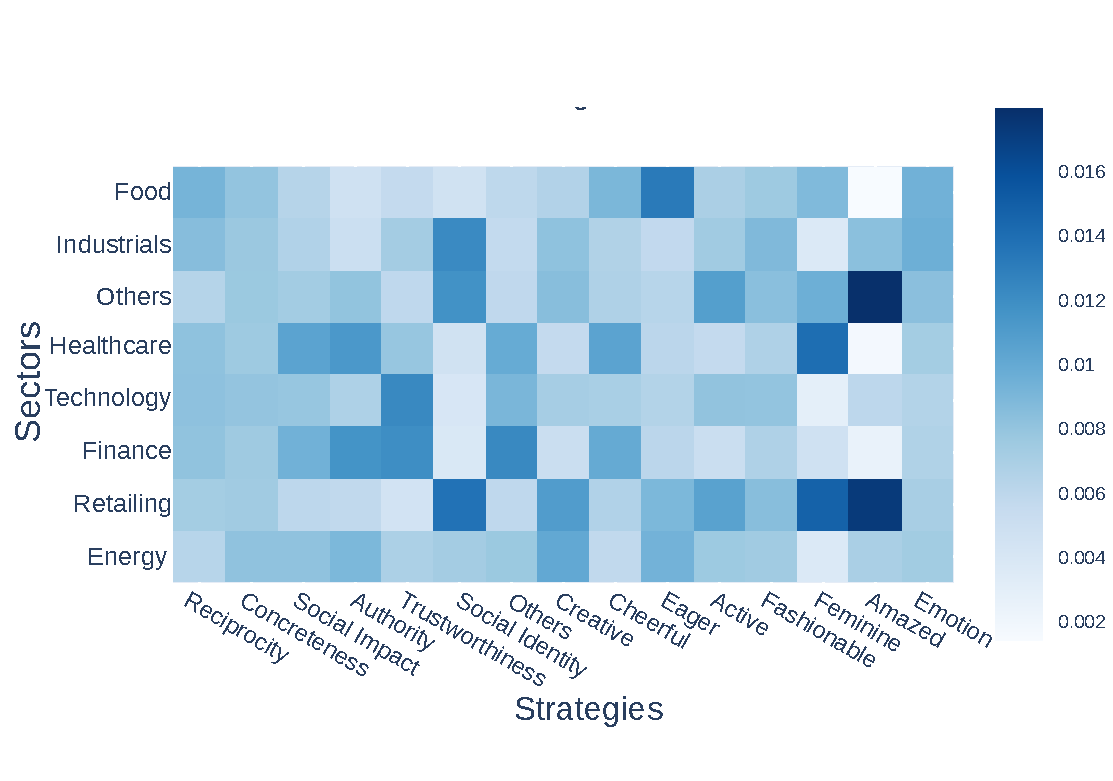
\includegraphics[scale =0.5]{images/correlation_sector_strategies.pdf}
            \caption{Dice correlation between company sectors and strategies.}
            \label{fig:correlation-between-company-sector-and-strategies}
            % \vspace*{-3mm}
    \end{figure}
\end{comment}

    
% \begin{figure*}
%         \centering
%         \begin{subfigure}[b]{0.75\textwidth}\centering
%         \includegraphics[scale=0.8]{images/us_heatmap_1.pdf}
%         \caption{US Heat Maps}
%         \end{subfigure}
%         % \vspace*{-3mm}
%     \end{figure*}
%     \begin{figure*}\ContinuedFloat
%         \centering
%         \begin{subfigure}[b]{0.75\textwidth}\centering
%         \includegraphics[scale=0.8]{images/us_heatmap_2.pdf}
%         \caption{US Heat-Maps}
%         \end{subfigure}
%         % \vspace*{-3mm}
%         \label{fig:us-heatmaps}
%     \end{figure*}

% \begin{table}[]
%         \centering
%         \begin{tcolorbox}[tab1,tabularx={YYYYY}]
%                 \toprule
%                 \textbf{\thead{Train \\Sample\\size}} & \textbf{\thead{Top-1 \\Accuracy}} & \textbf{\thead{Top-3 \\Accuracy}} &  \textbf{Recall} & \textbf{Precision} \\ \midrule
%                  1000 & 49.6 & 70.4 & 57.42 & \\ \midrule
%                  1250 & 50 &  73.2 & 59.07 & \\ \midrule
%                  1500 & 50.8 & 74.4 & 60.71 & \\ \midrule
%                  1750 & 50.8 & 76.4 & 62.36 & \\ \midrule
%                  2000 & 50 & 78 & 63.74 & \\ \midrule
%                  2250 & 50 & 75.6 & 63.74 & \\ \midrule
%                  2500 & 50.9 & 73.6 & 61.54 & \\\midrule
%         \end{tcolorbox}
%         \caption{Strategy prediction results on validation set}
%         \label{tab:my_label}
%     \end{table}
    
% \begin{table}[]
%         \centering
%         \begin{tcolorbox}[tab1,tabularx={YYYYY}]
%                 \toprule
%                  \textbf{\thead{Train \\Sample\\size}} & \textbf{\thead{Top-1 \\Accuracy}} & \textbf{\thead{Top-3 \\Accuracy}} &  \textbf{Recall} & \textbf{Precision} \\ \midrule
%                  1000 & 44 & 74.4 & 61.69 & 35.6 \\ \midrule
%                  1250 & 48.8 & 77.6 & 62.35 & 34.9\\ \midrule
%                  1500 & 52 & 76.4 & 62.00& 36.7 \\ \midrule
%                  1750 & 54.4 & 80.4 & 65.32 & 38.08 \\ \midrule
%                  2000 & 55.2 & 80.8 & 69.88 & 38.7\\ \midrule
%                  2250 & 58 & 80.8 & 72.06&40.00 \\ \midrule
%                  2500 & 59.2 & 84.8 & 74.59 &40.88 \\\bottomrule
%         \end{tcolorbox}
%         \caption{Strategy prediction results on test set}
%         \label{tab:my_label}
%     \end{table}
    


% \begin{table}[]
%     \small
%         \centering
%         \toprule
%         %\begin{adjustbox}{width=\columnwidth,center}
%         \resizebox{\columnwidth}{!}{%
%       \begin{tabular}{lll}%[tab1,tabularx={XYYYYY}]
%              \textbf{\thead{Models}} & \textbf{\thead{Top-1  Accuracy}} & \textbf{\thead{Top-3 Accuracy}}\\ \midrule
%              Our Model & 59.2 & 84.8 \\ \midrule
%              Without DenseCap & 55.6 & 80.8 \\ \midrule
%              Without Symbol   & 58.8 & 81.6 \\ \midrule
%           Without DenseCap\\\& Symbol & 55.2 & 80.8 \\ \midrule
%             Without OCR & 54.8 & 82 \\ \midrule
%             Without Symbol,\\OCR \& DenseCap & 58 & 78.8 \\ \midrule
%                  With Topic & 43.2 & 67.2 \\ \bottomrule
%         \end{tabular}}
%         \caption{\small  Effect of excluding different Modalities}
%         \vspace*{-3mm}
%         %\end{adjustbox}
%     \end{table}

%\begin{figure}[t]
%        \centering
%        \includegraphics[scale =0.2]{images/RandomSelection_vs_ActiveLearning.pdf}
%        \caption{Active Learning vs Random Selection}        \label{fig:AL_batch_test_discard}
%    \end{figure}





%%%%%%%%%%%%%%%%%%%%%%%%%%%%%%%%%%%%%%%%
%%%%%%%%%%%%%%%%%%%%%%%%%%%%%%%%%%%%%%%%
%%%%%%%%%%%%%%%%%%%%%%%%%%%%%%%%%%%%%%%%
%%%%%%%%%%%%%%%%%%%%%%%%%%%%%%%%%%%%%%%%
%%%%%%%%%%%%%%%%%%%%%%%%%%%%%%%%%%%%%%%%
%%%%%%%%%%%%%%%%%%%%%%%%%%%%%%%%%%%%%%%%
%%%%%%%%%%%%%%%%%%%%%%%%%%%%%%%%%%%%%%%%
%%%%%%%%%%%%%%%%%%%%%%%%%%%%%%%%%%%%%%%%
%%%%%%%%%%%%%%%%%%%%%%%%%%%%%%%%%%%%%%%%
%%%%%%%%%%%%%%%%%%%%%%%%%%%%%%%%%%%%%%%%
%%%%%%%%%%%%%%%%%%%%%%%%%%%%%%%%%%%%%%%%
%%%%%%%%%%%%%%%%%%%%%%%%%%%%%%%%%%%%%%%%
%%%%%%%%%%%%%%%%%%%%%%%%%%%%%%%%%%%%%%%%
%%%%%%%%%%%%%%%%%%%%%%%%%%%%%%%%%%%%%%%%
%%%%%%%%%%%%%%%%%%%%%%%%%%%%%%%%%%%%%%%%
%%%%%%%%%%%%%%%%%%%%%%%%%%%%%%%%%%%%%%%%
%%%%%%%%%%%%%%%%%%%%%%%%%%%%%%%%%%%%%%%%
%%%%%%%%%%%%%%%%%%%%%%%%%%%%%%%%%%%%%%%%
\chapter{Content and Behavior Models}
\label{chatper:Content and Behavior Models}




%%%%%%%%%%%%%%%%%%%%%%%%%%%%%%%%%%%%%%%%
%%%%%%%%%%%%%%%%%%%%%%%%%%%%%%%%%%%%%%%%
%%%%%%%%%%%%%%%%%%%%%%%%%%%%%%%%%%%%%%%%
%%%%%%%%%%%%%%%%%%%%%%%%%%%%%%%%%%%%%%%%
%%%%%%%%%%%%%%%%%%%%%%%%%%%%%%%%%%%%%%%%
%%%%%%%%%%%%%%%%%%%%%%%%%%%%%%%%%%%%%%%%
%%%%%%%%%%%%%%%%%%%%%%%%%%%%%%%%%%%%%%%%
%%%%%%%%%%%%%%%%%%%%%%%%%%%%%%%%%%%%%%%%
%%%%%%%%%%%%%%%%%%%%%%%%%%%%%%%%%%%%%%%%
%%%%%%%%%%%%%%%%%%%%%%%%%%%%%%%%%%%%%%%%
%%%%%%%%%%%%%%%%%%%%%%%%%%%%%%%%%%%%%%%%
%%%%%%%%%%%%%%%%%%%%%%%%%%%%%%%%%%%%%%%%
%%%%%%%%%%%%%%%%%%%%%%%%%%%%%%%%%%%%%%%%
%%%%%%%%%%%%%%%%%%%%%%%%%%%%%%%%%%%%%%%%
%%%%%%%%%%%%%%%%%%%%%%%%%%%%%%%%%%%%%%%%
%%%%%%%%%%%%%%%%%%%%%%%%%%%%%%%%%%%%%%%%
%%%%%%%%%%%%%%%%%%%%%%%%%%%%%%%%%%%%%%%%
%%%%%%%%%%%%%%%%%%%%%%%%%%%%%%%%%%%%%%%%
%%%%%%%%%%%%%%%%%%%%%%%%%%%%%%%%%%%%%%%%
%%%%%%%%%%%%%%%%%%%%%%%%%%%%%%%%%%%%%%%%
\chapter{Generating Content Leading to Optimal Behavior}
\label{chatper:Generating Content Leading to Optimal Behavior}


%%%%%%%%%%%%%%%%%%%%%%%%%%%%%%%%%%%%%%%%
%%%%%%%%%%%%%%%%%%%%%%%%%%%%%%%%%%%%%%%%
\chapter*{Publications}
\begin{enumerate}
    \item Khurana, V., Kumar, Y., Hollenstein, N., Kumar, R., \& Krishnamurthy, B. (2023). Synthesizing Human Gaze Feedback for Improved NLP Performance. In Proceedings of the 17th Conference of the European Chapter of the Association for Computational Linguistics (pp. 1895-1908).
    
    \item Kumar, Y., Jha, R., Gupta, A., Aggarwal, M., Garg, A., Malyan, T., Bhardwaj, A., Ratn Shah, R., Krishnamurthy, B., \& Chen, C. (2023). Persuasion Strategies in Advertisements. Proceedings of the AAAI Conference on Artificial Intelligence, 37(1), 57-66. \url{https://doi.org/10.1609/aaai.v37i1.25076}

    \item Bhattacharya, A., Singla, Y. K., Krishnamurthy, B., Shah, R. R., \& Chen, C. (2023). A Video Is Worth 4096 Tokens: Verbalize Story Videos To Understand Them In Zero Shot. In Proceedings of the 2023 Conference on Empirical Methods in Natural Language Processing, pages 9822–9839, Singapore. Association for Computational Linguistics.

    \item Khandelwal, A., Agrawal, A., Bhattacharyya, A., Singla, Y.K., Singh, S., Bhattacharya, U., Dasgupta, I., Petrangeli, S., Shah, R.R., Chen, C. and Krishnamurthy, B., 2023. Large Content And Behavior Models To Understand, Simulate, And Optimize Content And Behavior. arXiv preprint arXiv:2309.00359. (Under review at ICLR-24). 

    \item  S I, H., Singh, S., K Singla, Y., Krishnamurthy, B., Chen, C., Baths V., \& Ratn Shah, R. (2023). Sharingan: How Much Will Your Customers Remember Your Brands After Seeing Your Ads?. arxiv preprint (Under review at NAACL-24).

    \item Khurana, V., Singla, Y.K., Subramanian, J., Shah, R.R., Chen, C., Xu, Z. and Krishnamurthy, B., 2023. Behavior Optimized Image Generation. arXiv preprint arXiv:2311.10995. (Under review at CVPR-24)

\end{enumerate}


%%%%%%%%%%%%%%%%%%%%%%%%%%%%%%%%%%%%%%%%
%%%%%%%%%%%%%%%%%%%%%%%%%%%%%%%%%%%%%%%%
%%%%%%%%%%%%%%%%%%%%%%%%%%%%%%%%%%%%%%%%
\bibliographystyle{unsrt}
\bibliography{ref}
\addcontentsline{toc}{chapter}{Bibliography}

\end{document}
